\documentclass{beamer}
\usetheme{Warsaw}
% \usetheme{metropolis}
\setbeamertemplate{footline}[page number]
% \setbeamertemplate{headline}{}
\setbeamercolor{page number in head/foot}{fg=black}
\setbeamerfont{page number in head/foot}{size=\footnotesize}
\setbeamertemplate{navigation symbols}{}

\setbeamertemplate{section in toc}{\hspace*{1em}\inserttocsectionnumber.~\inserttocsection\par}

\usepackage[backend=biber, style=authoryear, backref=true, hyperref=true]{biblatex}
\addbibresource{biblio.bib}
\renewcommand*{\bibfont}{\scriptsize}

\usepackage{version}
\usepackage[utf8]{inputenc}
% \usepackage[french]{babel}
\usepackage[T1]{fontenc}
\usepackage{amsmath,mathtools}
\usepackage{amssymb}
\usepackage{amsthm}
\usepackage{bbm}
\usepackage{relsize}
\usepackage{multirow}
\usepackage{hyperref}
\hypersetup{colorlinks=true, citecolor=green, linkcolor=blue, urlcolor=blue}
\usepackage{color}
\definecolor{darkgreen}{HTML}{3C8031}

\usepackage[skip=2pt]{caption}
\captionsetup[figure]{labelformat=empty}

\usepackage{tikz}
% \usetikzlibrary{shapes,positioning,arrows,shapes.arrows, decorations.markings,arrows.meta,decorations.pathreplacing}
\usetikzlibrary{backgrounds,decorations.pathreplacing,calc,tikzmark}
\newcommand{\AxisRotator}[1][rotate=0]{%
    \tikz [x=0.4cm,y=0.60cm,line width=.2ex,-stealth,#1]
    \draw (-54,-5.5) arc (-150:150:1 and 1);%
}

\setbeamertemplate{headline}{}

\addtobeamertemplate{block begin}{%
  \setlength{\textwidth}{1.05\textwidth}%
}{}

\setlength{\abovedisplayskip}{0pt}
\setlength{\belowdisplayskip}{0pt}
\setlength{\abovedisplayshortskip}{0pt}
\setlength{\belowdisplayshortskip}{0pt}
\setlength{\jot}{0pt}

\newcommand{\gw}{\text{GW}}
\newcommand{\ot}{\text{OT}}
\newcommand{\coot}{\text{COOT}}
\newcommand{\ugw}{\text{UGW}}
\newcommand{\agw}{\text{AGW}}
\newcommand{\uot}{\text{UOT}}
\newcommand{\ucoot}{\text{UCOOT}}
\newcommand{\fgw}{\text{FGW}}
\newcommand{\fugw}{\text{FUGW}}
\newcommand{\kl}{\text{KL}}
\newcommand{\gh}{\text{GH}}

\newcommand{\cX}{\mathcal X}
\newcommand{\cY}{\mathcal Y}
\newcommand{\cM}{\mathcal M}
\newcommand{\cE}{\mathcal E}
\newcommand{\cL}{\mathcal L}
\newcommand{\cP}{\mathcal P}
\newcommand{\bbR}{\mathbb R}
\newcommand{\rmd}{\mathrm{d}}
\newcommand{\bX}{\textbf{X}}
\newcommand{\bY}{\textbf{Y}}

\newcommand{\pis}{{\color{blue}{\pi^s}}}
\newcommand{\pif}{{\color{red}{\pi^f}}}

\newcommand{\mfsrc}{{\color{red}{\mu_1^f}}}
\newcommand{\mftg}{{\color{red}{\mu_2^f}}}
\newcommand{\mssrc}{{\color{blue}{\mu_1^s}}}
\newcommand{\mstg}{{\color{blue}{\mu_2^s}}}
\newcommand{\sfspace}{{\color{blue}{s.}}{\color{red}{f. }}}

\newcommand{\source}{{\color{red}{\mathcal X}}}
\newcommand{\target}{{\color{blue}{\mathcal Y}}}
\newcommand{\redx}{{\color{red}{x}}}
\newcommand{\bluey}{{\color{blue}{y}}}

\setlength{\leftmargini}{0.2cm}
\setlength{\leftmarginii}{0.1cm}

\newtheorem{proposition}{Proposition}[section]
\newtheorem{assumption}{Assumption}

%%%%%%%%%%%%%%%%%%%%%%%%%%%%%%
%%%%%%%%%%%%%%%%%%%%%%%%%%%%%%

%Information to be included in the title page:
\title[PhD Defense]{Optimal Transport for Transfer Learning \break Across Spaces}

\author[]{Quang Huy Tran \break \break \scriptsize{Under the supervision of Nicolas Courty, Karim Lounici and Rémi Flamary}}
\titlegraphic{
  % \hspace{-0.3cm}
  
\includegraphics[height=0.7cm, keepaspectratio=true]{OT_new/logo_irisa.png}\hspace{0.2cm}~
  
\includegraphics[height=0.9cm, keepaspectratio=true]{OT_new/logo_univ_bret.png}\hspace{0.2cm}~
  
\includegraphics[height=1cm, keepaspectratio=true]{OT_new/logo_cmap.png}\hspace{0.2cm}~
  
\includegraphics[height=1cm, keepaspectratio=true]{OT_new/logo_x_ipp.png}\hspace{0.2cm}
}

% \institute[] % (optional)
% {
%   \inst{1}%
%   Institut de Recherche en Informatique et Systèmes Aléatoires - IRISA \\
%   Université Bretagne Sud
%   \and
%   \inst{2}%
%   Centre de Mathématiques Appliquées - CMAP \\
%   Ecole Polytechnique
% }

\date[]{PhD Defense, 16 May 2024, Palaiseau}

\begin{document}

\begin{frame}
  \titlepage
\end{frame}

\AtBeginSection[]
{
  \begin{frame}
    \frametitle{Table of Contents}
    \bf{\tableofcontents[currentsection]}
  \end{frame}
}

% %%%%%%%%%%%%%%%%%%%%%%%%%%%%%%%%%%%%%%
% \begin{frame}{Cross-domain alignment}
% \scriptsize
% \begin{minipage}[t]{0.6\linewidth}
%   \vspace{0cm}
%   {\color{brown}{\textbf{OT = comparison of weighted spaces}.}}
%   \begin{itemize}
%     \item[$\bullet$] OT-based divergence
%     $\Rightarrow$ Density fitting.
%     \item[$\bullet$] Transport {\color{darkgreen}{\textbf{plan}}}/map
%     $\Rightarrow$ {\color{darkgreen}{\textbf{Alignments}}}/mappings.
%   \end{itemize}

%   \vspace{0.3cm}
%   {\color{brown}{\textbf{Classical setting:}}} metric-measure spaces
%   \hfill\tikzmark{right}
%   \begin{itemize}
%     \item[$\bullet$] Source: ${\color{red}{\cX = (X, d, \mu_X)}}$. \tikzmark{2nd}
%     \item[$\bullet$] Target: ${\color{blue}{\cY = (Y, d, \mu_Y)}}$. \tikzmark{4th}
%   \end{itemize}
%   \vspace{-0.3cm}
%   \begin{align*}
%     W_p^p (\source, \target) =
%     \inf_{\pi \in U({\color{red}{\mu_X}}, {\color{blue}{\mu_Y}})}
%     \int d(\redx, \bluey)^p \; \rmd\pi(\redx, \bluey).
%   \end{align*}
%   \begin{tikzpicture}[overlay, remember picture]
%     \node[anchor=base] (a) at (pic cs:2nd) {\vphantom{h}}; % push the mark to the top of the line (ie including ascenders)
%     \node[anchor=base] (b) at (pic cs:4th) {\vphantom{g}}; % push the mark to the bottom of the line (ie including descenders)
%     \draw [decoration={brace,amplitude=0.5em},decorate,thick,black]
%      (a.north) -- (b.south);
%   \end{tikzpicture}
%   \begin{tikzpicture}[remember picture, overlay]
%     \node[shift={(-0.7cm,1.15cm)}] at (current page.center)
%     {$\Rightarrow$ sharing metric};
%   \end{tikzpicture}

%   \end{minipage}%'
%   \hfill%
%   \hspace{-6cm}
%   \begin{minipage}[t]{0.49\linewidth}
%     \vspace{-0.2cm}
%     \begin{tikzpicture}[remember picture, overlay]
%       \node[shift={(3.2cm,1.8cm)}] at (current page.center)
%       {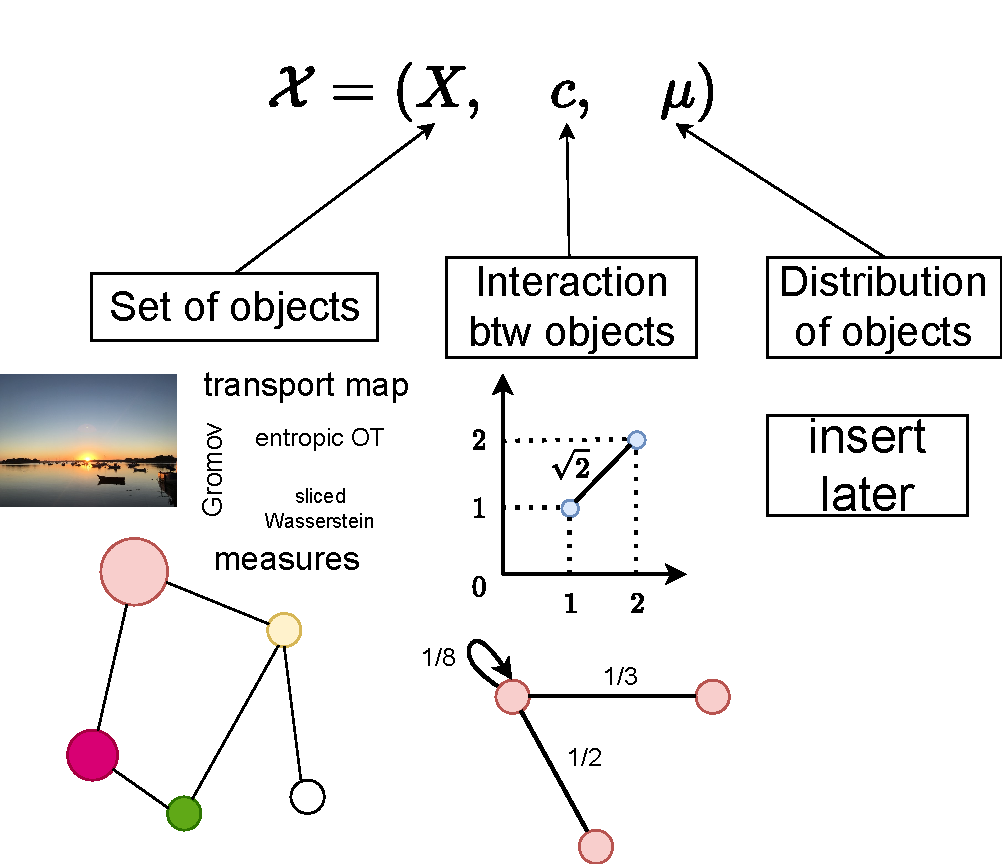
\includegraphics[scale=0.3]{OT_new/intro.pdf}};
%     \end{tikzpicture}
%   \end{minipage}

%   \vspace{-0.1cm}
%   {\color{brown}{\textbf{How to do the transport if:}}}
%   \begin{itemize}
%     \item[$\bullet$] Incomparable spaces: ${\color{red}{d}} \neq {\color{blue}{d}} \Rightarrow$
%     What does $d(\redx, \bluey)$ mean?
%     \item[$\bullet$] "Partially" comparable spaces: ${\color{red}{X = X_1 \cup X_2}}, {\color{blue}{Y = Y_1 \cup Y_2}}$,
%     where ${\color{red}{X_2}}, {\color{blue}{Y_2}} \subset (E, d)$.
%     \item[$\bullet$] Align everything?
%     \item[$\bullet$] Interaction(image, image) $\Rightarrow$ Can we do Interaction(image, text)?
%   \end{itemize}

%   \begin{figure}
%     \centering
%     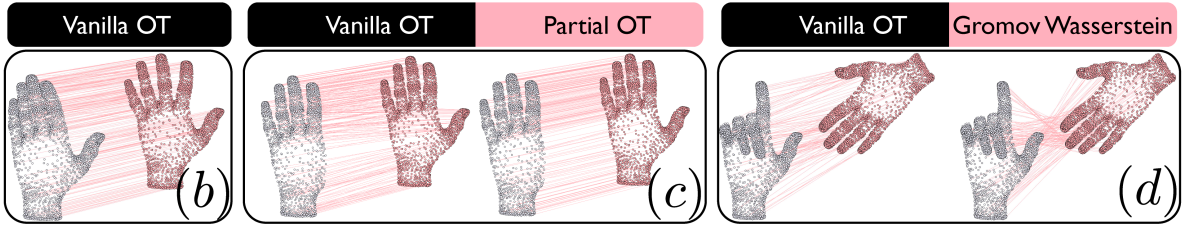
\includegraphics[scale=0.25]{OT_new/intro_ot.png}
%     \caption*{\scriptsize{Cite here}}
%   \end{figure}
%   % \begin{tikzpicture}[remember picture, overlay]
%   %   \node[shift={(0cm,-3.5cm)}] at (current page.center)
%   %   {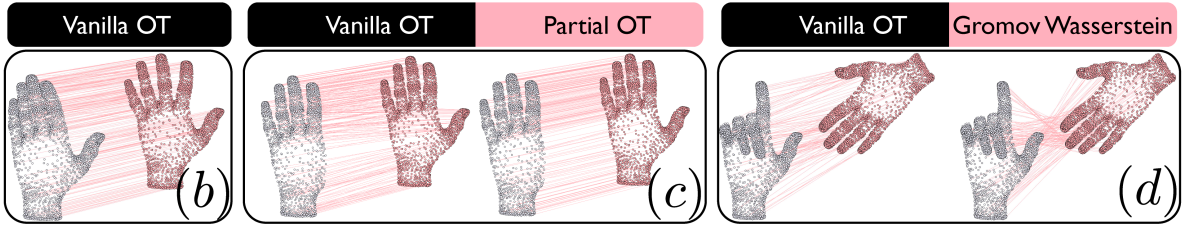
\includegraphics[scale=0.2]{OT_new/intro_ot.png}};
%   % \end{tikzpicture}

% \end{frame}

% \begin{frame}{Cross-domain alignment}

%   \vspace{-0.5cm}
%   \begin{figure}
%     \centering
%     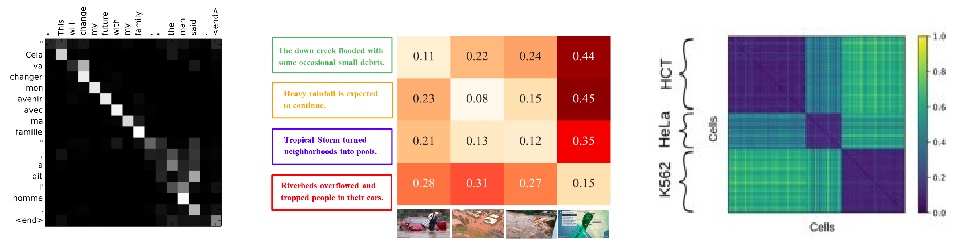
\includegraphics[width=1.05\linewidth, keepaspectratio=true]{OT_new/intro_new1.pdf}
%     \vspace{-0.5cm}
%     % \caption*{\scriptsize{Examples: ,
%     % image-text summary \footnote{\tiny{\parencite{Qiu23}}}, cell alignment \footnote{\tiny{\parencite{Huizing22a}}}}}
%   \end{figure}

%   % \begin{tikzpicture}[remember picture, overlay]
%   %   \node[shift={(0cm,1.8cm)}] at (current page.center)
%   %   {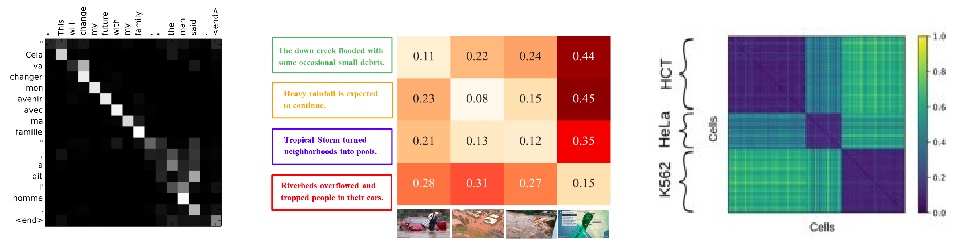
\includegraphics[scale=0.75]{OT_new/intro_new1.pdf}};
%   % \end{tikzpicture}

%   \begin{tikzpicture}[remember picture, overlay]
%     \node[shift={(-3.6cm,0.75cm)}, text width=0.3\linewidth] at (current page.center)
%     {\scriptsize{Machine translation \footnotemark}};
%   \end{tikzpicture}
%   \footnotetext[1]{\tiny{\parencite{Bahdanau15}}}

%   \begin{tikzpicture}[remember picture, overlay]
%     \node[shift={(0.6cm,0.75cm)}, text width=0.4\linewidth] at (current page.center)
%     {\scriptsize{Image-text summary \footnotemark}};
%   \end{tikzpicture}
%   \footnotetext[2]{\tiny{\parencite{Qiu23}}}

%   \begin{tikzpicture}[remember picture, overlay]
%     \node[shift={(5.5cm,0.75cm)}, text width=0.4\linewidth] at (current page.center)
%     {\scriptsize{Cell alignment \footnotemark}};
%   \end{tikzpicture}
%   \footnotetext[3]{\tiny{\parencite{Huizing22a}}}

%   \vspace{-1.3cm}
%   \begin{figure}
%     \centering
%     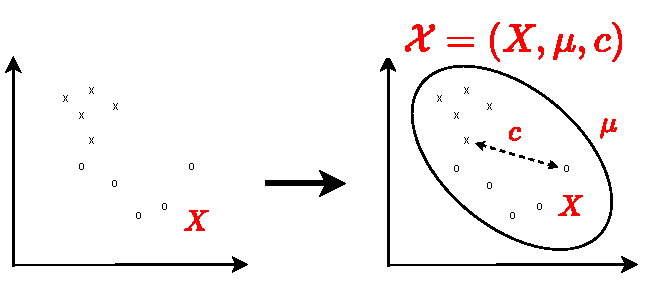
\includegraphics[width=0.75\linewidth, keepaspectratio=true]{OT_new/intro_new2.pdf}
%     \vspace{-0.2cm}
%     \caption*{\scriptsize{Abstraction of weighted space.}}
%   \end{figure}

% \end{frame}

%%%%%%%%%%%%%%%%%%%%%%%%%%%%%%%%%%%%%%%%%%%%%%
% \begin{frame}{Why Gromov-Wasserstein distance?}
% \scriptsize
%   \begin{align*}
%     d_{H} \big( {\color{blue}{(X, d)}}, {\color{red}{(Y, d)}} \big)
%     = \inf_{R \in \mathcal R({\color{blue}{X}}, {\color{red}{Y}})}
%     \sup_{(x, y) \in R} d(x, y)
%   \end{align*}

%   \begin{align*}
%     W_{\infty}\big( {\color{blue}{(X, \mu_X, d)}}, {\color{red}{(Y, \mu_Y, d)}} \big) =
%     \inf_{\pi \in U({\color{blue}{\mu_X}}, {\color{red}{\mu_Y}})} \sup_{(x,y) \in \text{supp}(\pi)}
%     d(x, y)
%   \end{align*}

%   \begin{align*}
%     W_p^p \big( {\color{blue}{(X, \mu_X, d)}}, {\color{red}{(Y, \mu_Y, d)}} \big)
%     = \inf_{\pi \in U({\color{blue}{\mu_X}}, {\color{red}{\mu_Y}})}
%     \int d(x, y)^p \; \rmd\pi(x, y).
%   \end{align*}

%   \begin{align*}
%     \gh\big( {\color{blue}{(X, d_X)}}, {\color{red}{(Y, d_Y)}} \big)
%     = \frac{1}{2} \inf_{R \in \mathcal R({\color{blue}{X}}, {\color{red}{Y}})}
%     \sup_{\substack{(x_1,y_1) \in R \\ (x_2,y_2) \in R}} \big| d_X(x_1, x_2) - d_Y(y_1, y_2) \big|
%   \end{align*}

%   \begin{align*}
%     \gw_{\infty}\big( {\color{blue}{(X, \mu_X, d_X)}}, {\color{red}{(Y, \mu_Y, d_Y)}} \big)
%     = \inf_{ \pi \in U({\color{blue}{\mu_X}}, {\color{red}{\mu_Y}})}
%     \sup_{\substack{(x_1,y_1) \in \text{supp}(\pi) \\ (x_2,y_2) \in \text{supp}(\pi)}}
%     \big| d_X(x_1, x_2) - d_Y(y_1, y_2) \big|.
%   \end{align*}

%   \begin{align*}
%     \gw_p^p\big( {\color{blue}{(X, \mu_X, d_X)}}, {\color{red}{(Y, \mu_Y, d_Y)}} \big)
%     = \inf_{ \pi \in U({\color{blue}{\mu_X}}, {\color{red}{\mu_Y}})}
%     \iint |d_X(x_1, x_2) - d_Y(y_1, y_2)|^p \;
%     \rmd\pi(x_1, y_1) \; \rmd\pi(x_2, y_2).
% \end{align*}
% \end{frame}

%%%%%%%%%%%%%%%%%%%%%%%%%%%%%%%%%%%%%%
\begin{frame}{Cross-domain alignment}
  \begin{figure}
    \centering
    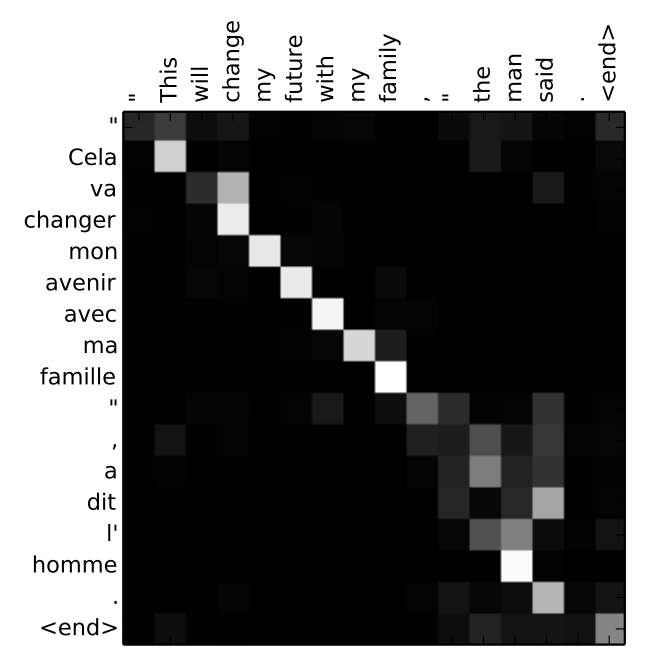
\includegraphics[width=0.65\linewidth, keepaspectratio=true]{OT_new/translation.png}
    \caption*{\scriptsize{Machine translation \parencite{Bahdanau15}}}
  \end{figure}
\end{frame}

%%%%%%%%%%%%%%%%%%%%%%%%%%%%%%%%%%%%%%
\begin{frame}{Cross-domain alignment}
  \begin{figure}
    \centering
    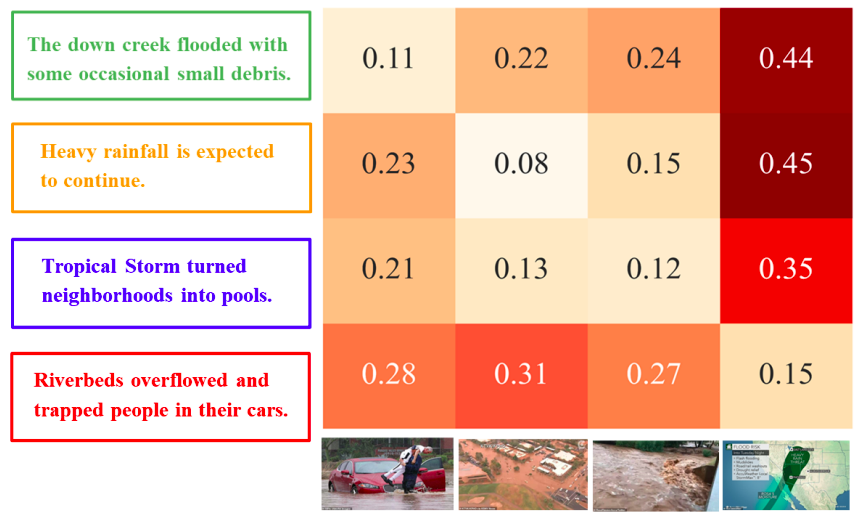
\includegraphics[width=0.7\linewidth, keepaspectratio=true]{OT_new/img2text.png}
    \caption*{\scriptsize{Image-text summary \parencite{Qiu23}}}
  \end{figure}
\end{frame}

%%%%%%%%%%%%%%%%%%%%%%%%%%%%%%%%%%%%%%
\begin{frame}{Cross-domain alignment}
  \begin{figure}
    \centering
    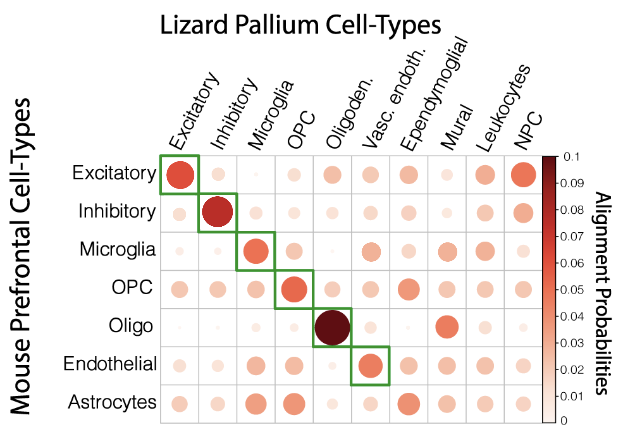
\includegraphics[width=0.7\linewidth, keepaspectratio=true]{OT_new/xSp_cellAlign.png}
    \caption*{\scriptsize{Cell alignments \parencite{Demetci23}}}
  \end{figure}
\end{frame}

%%%%%%%%%%%%%%%%%%%%%%%%%%%%%%%%%%%%%%
\begin{frame}{Cross-domain alignment}
  \begin{figure}
    \centering
    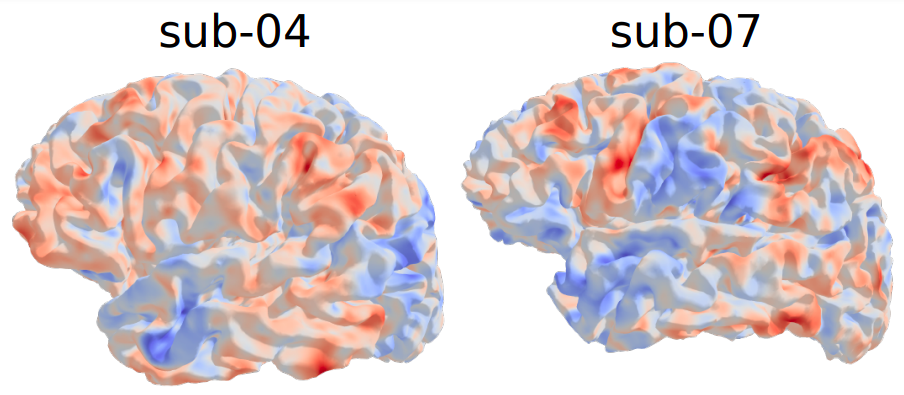
\includegraphics[width=0.7\linewidth, keepaspectratio=true]{OT_new/brain.png}
    \caption*{\scriptsize{Human brain alignments \parencite{Thual22}}}
  \end{figure}
\end{frame}

%%%%%%%%%%%%%%%%%%%%%%%%%%%%%%%%%%%%%%
\begin{frame}{Alignment with Optimal transport}
  \vspace*{0.5cm}
  \scriptsize
  \begin{itemize}
    \setlength\itemsep{0.5cm}

    \item[$\bullet$] {\color{brown}{\textbf{Transport plan:}}}
    $\ot(\cX_1, \cX_2) = \inf_{\pi} \cL_{OT}(\pi)$.
    \vspace*{0.2cm}
    \begin{enumerate}
      \scriptsize
      \setlength\itemindent{10pt}
      \setlength\itemsep{0.2cm}
      \item[1.] Position of alignments.
      \item[2.] Importance of alignments.
    \end{enumerate}
    \item[$\bullet$] {\color{brown}{\textbf{Inputs of OT:}}} weighted spaces.
  \end{itemize}

  \vspace*{-1cm}
  \begin{figure}
    \centering
    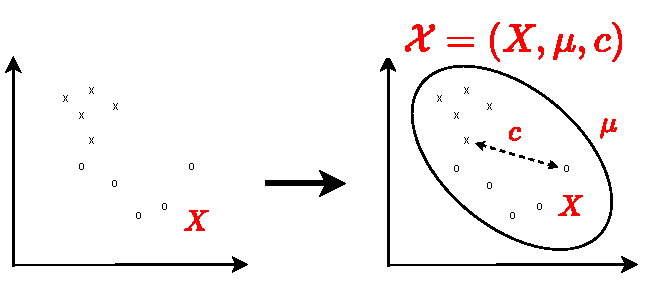
\includegraphics[width=0.65\linewidth, keepaspectratio=true]{OT_new/intro_new2.pdf}
    \vspace*{-1.2cm}
    \caption*{\scriptsize{Abstraction of weighted space.}}
  \end{figure}

  \begin{tikzpicture}[remember picture, overlay]
    \node[shift={(-4cm,-5.5cm)}] at (current page.center)
    {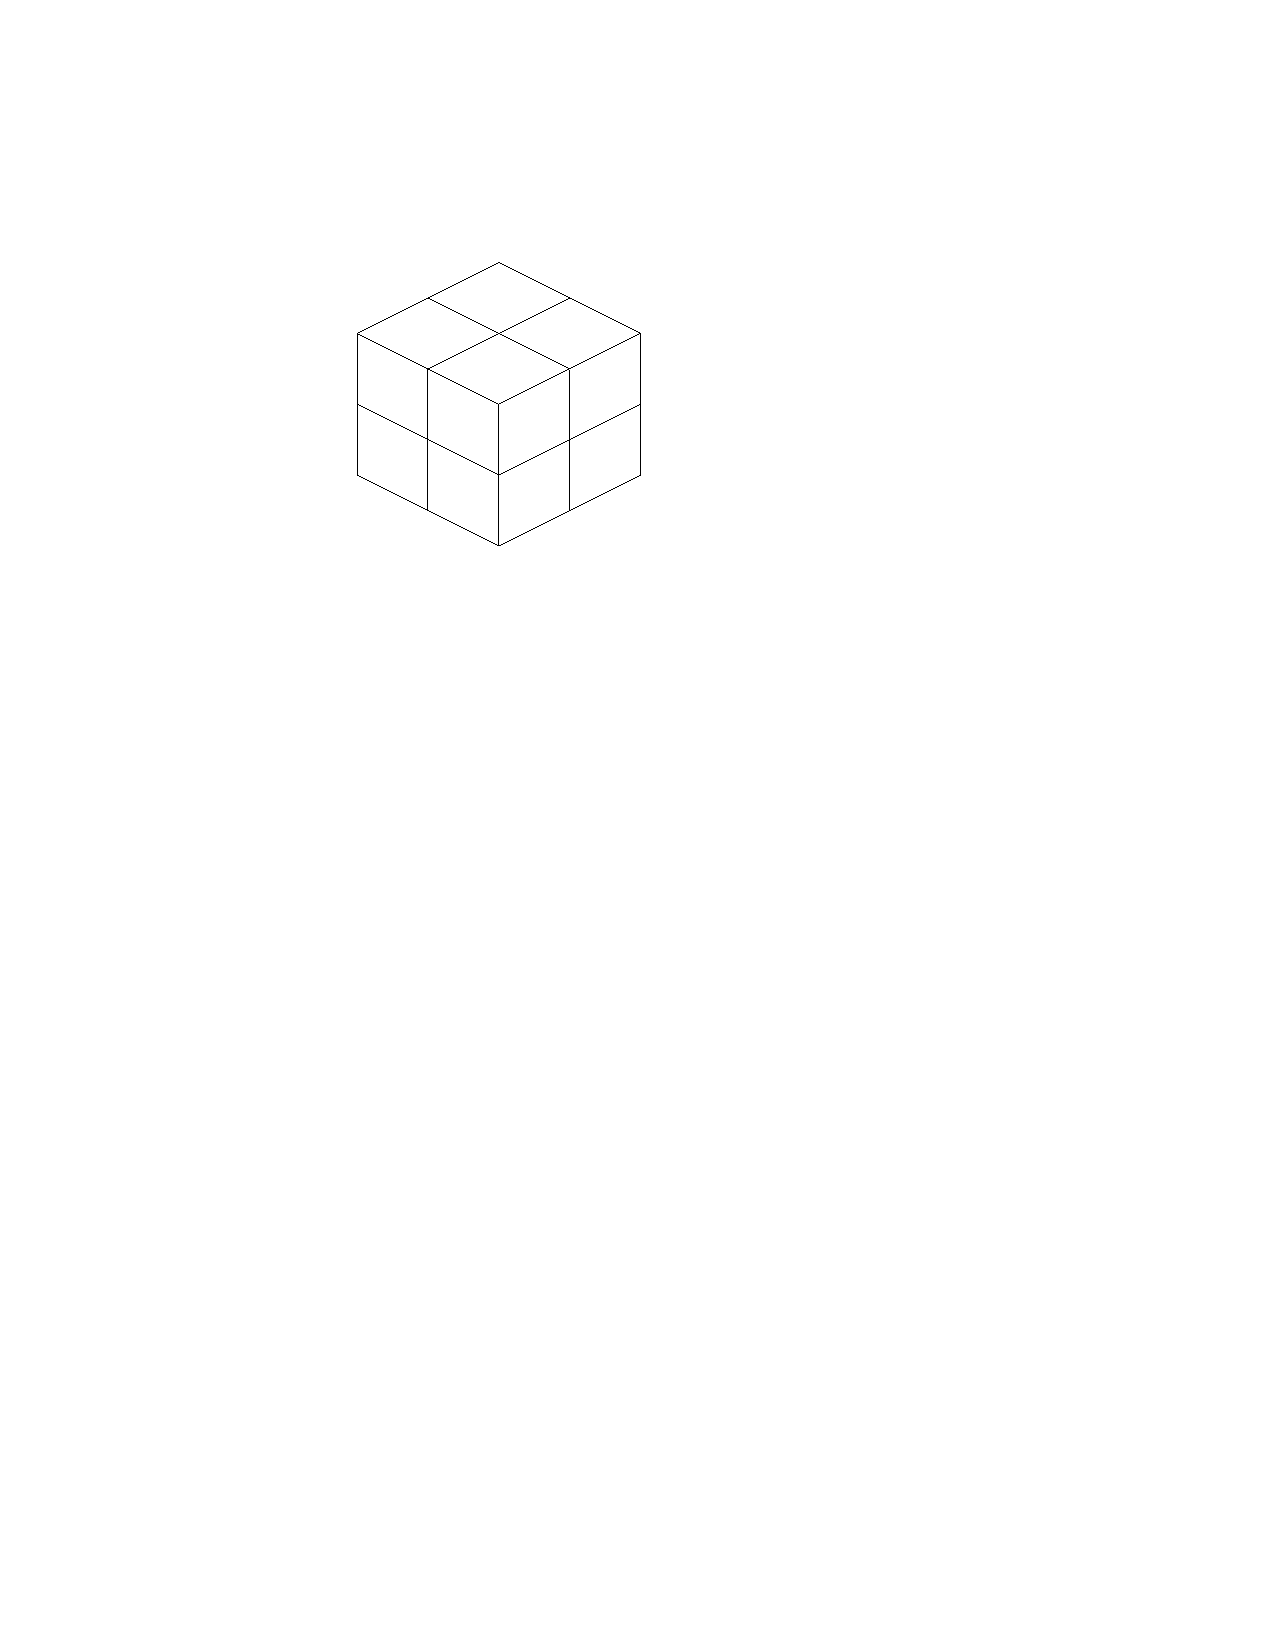
\includegraphics[scale=0.35]{OT_new/cube_empty.pdf}};
  \end{tikzpicture}
\end{frame}

%%%%%%%%%%%%%%%%%%%%%%%%%%%%%%%%%%%%%
\begin{frame}{Cross-domain alignment with Optimal transport}
  \vspace{-0.6cm}
  \scriptsize
  \begin{block}{Gromov-Wasserstein distance \parencite{Memoli07,Memoli11}}
  The GW distance of order $p \geq 1$ between two metric-measure spaces
  $\cX_1 = (X_1, \mu_1, d_1)$ and $\cX_2 = (X_2, \mu_2, d_2)$ is defined as
  \begin{align*}
    \gw_p^p(\cX_1, \cX_2) = \inf_{\pi \in U(\mu_1, \mu_2)}
    \iint \left| d_1({\color{blue}{x_1}}, {\color{red}{x_1'}}) - d_2({\color{blue}{x_2}}, {\color{red}{x_2'}}) \right|^p
    \rmd\pi({\color{blue}{x_1, x_2}}) \; \rmd\pi({\color{red}{x_1', x_2'}}),
  \end{align*}
  where $U(\mu_1, \mu_2) = \{ \pi \in \mathcal P(X_1 \times X_2): \int_{X_2} \rmd\pi(\cdot, x_2) = \mu_1 \text{ and } \int_{X_1} \rmd\pi(x_1, \cdot) = \mu_2 \}$.
\end{block}

\begin{tikzpicture}[remember picture, overlay]
  \node[shift={(-4cm,-5.5cm)}] at (current page.center)
  {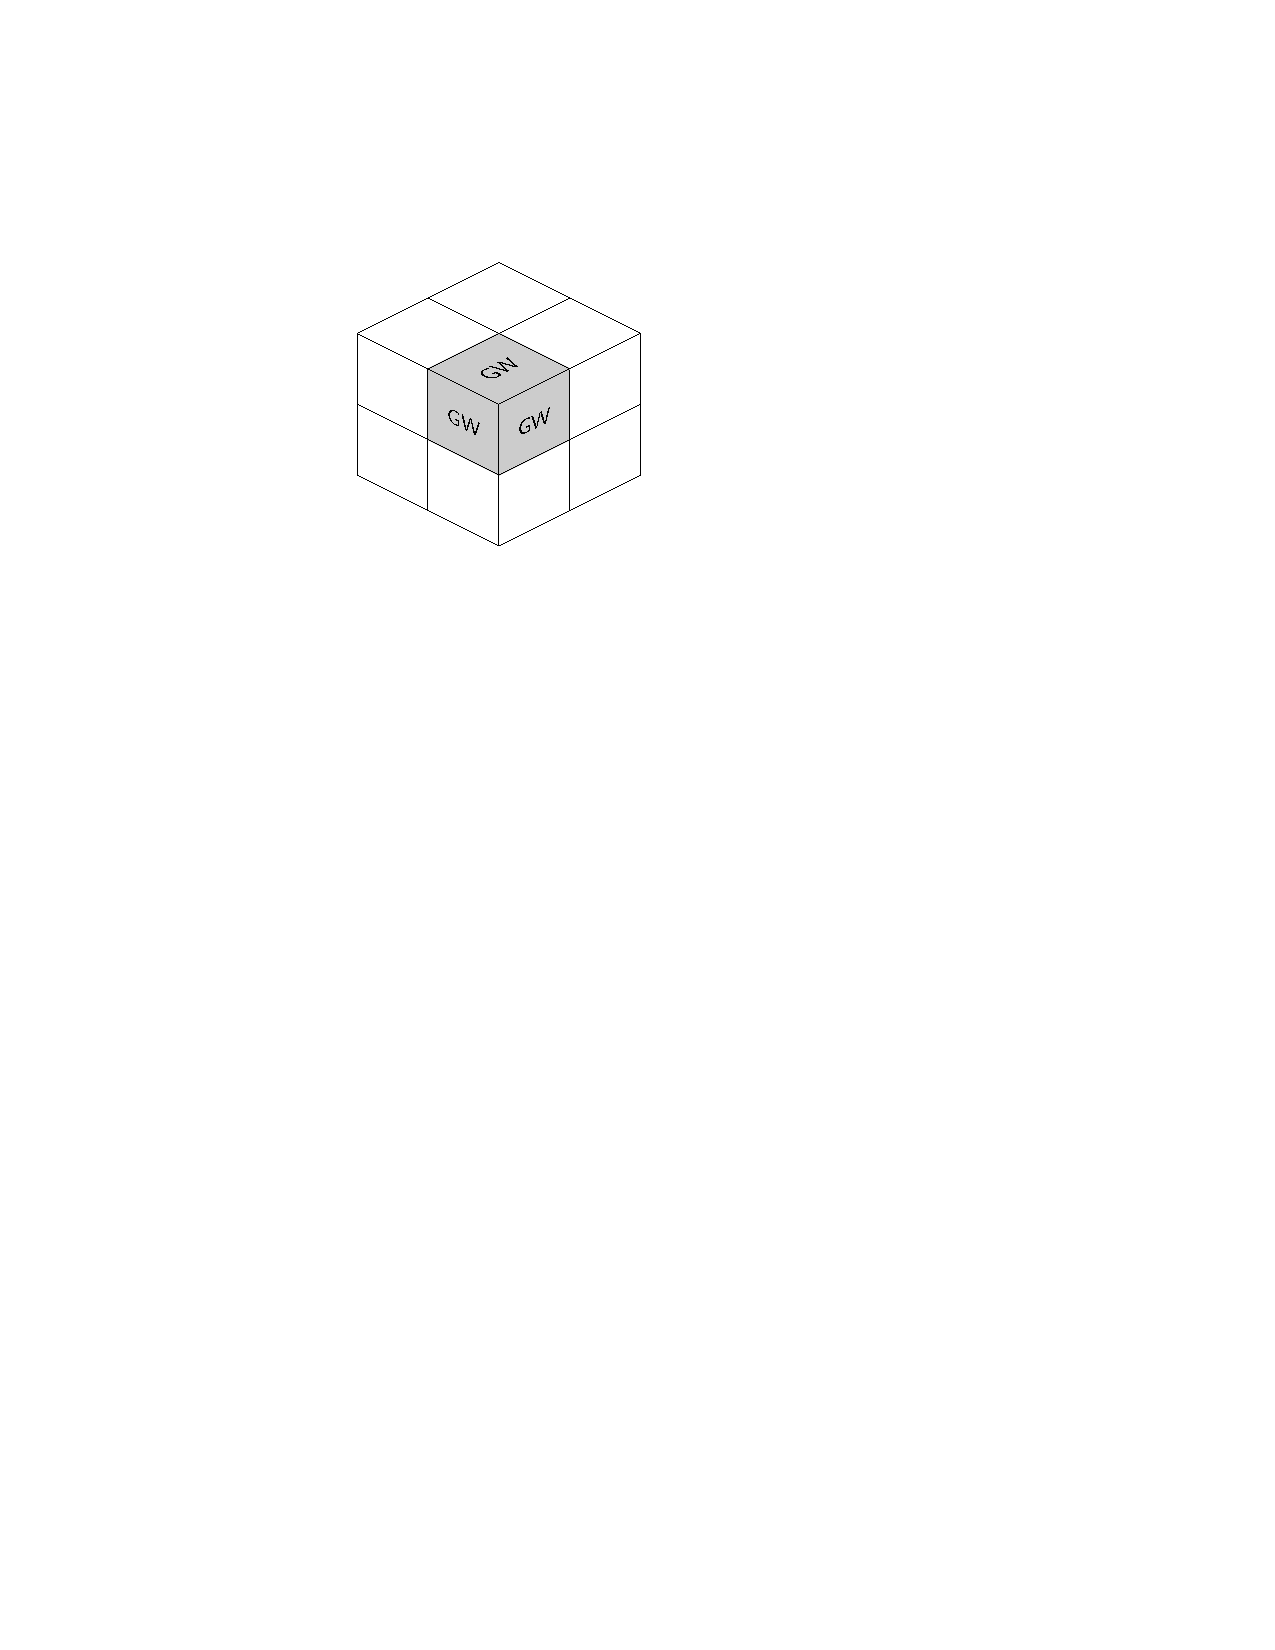
\includegraphics[scale=0.35]{OT_new/cube_gw.pdf}};
\end{tikzpicture}

\vspace{-0.3cm}
\begin{minipage}[t]{0.5\linewidth}
\begin{itemize}
  \item[$\bullet$] Metric properties
  \item[$\bullet$] Isometries.
  \item[$\bullet$] Quadratic and nonconvex problem.
\end{itemize}
\end{minipage}%
\hfill%
\hspace{-6cm}
\begin{minipage}[t]{0.55\linewidth}
  % \vspace{0.1cm}
\begin{figure}
  \centering
  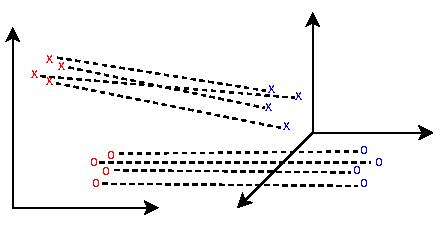
\includegraphics[width=1.2\linewidth, keepaspectratio=true]{OT_new/gw.pdf}
\end{figure}
\end{minipage}

\end{frame}

%%%%%%%%%%%%%%%%%%%%%%%%%%%%%%%%%%%%%
\begin{frame}{Cross-domain alignment with Optimal transport}
  \vspace{-0.6cm}
  \scriptsize
  \begin{block}{Gromov-Wasserstein distance \parencite{Memoli07,Memoli11}}
  The GW distance of order $p \geq 1$ between two metric-measure spaces
  $\cX_1 = (X_1, \mu_1, d_1)$ and $\cX_2 = (X_2, \mu_2, d_2)$ is defined as
  \begin{align*}
    \gw_p^p(\cX_1, \cX_2) = \inf_{\pi \in U(\mu_1, \mu_2)}
    \iint \left| d_1({\color{blue}{x_1}}, {\color{red}{x_1'}}) - d_2({\color{blue}{x_2}}, {\color{red}{x_2'}}) \right|^p
    \rmd\pi({\color{blue}{x_1, x_2}}) \; \rmd\pi({\color{red}{x_1', x_2'}}),
  \end{align*}
  where $U(\mu_1, \mu_2) = \{ \pi \in \mathcal P(X_1 \times X_2): \int_{X_2} \rmd\pi(\cdot, x_2) = \mu_1 \text{ and } \int_{X_1} \rmd\pi(x_1, \cdot) = \mu_2 \}$.
\end{block}

\begin{tikzpicture}[remember picture, overlay]
  \node[shift={(-4cm,-5.5cm)}] at (current page.center)
  {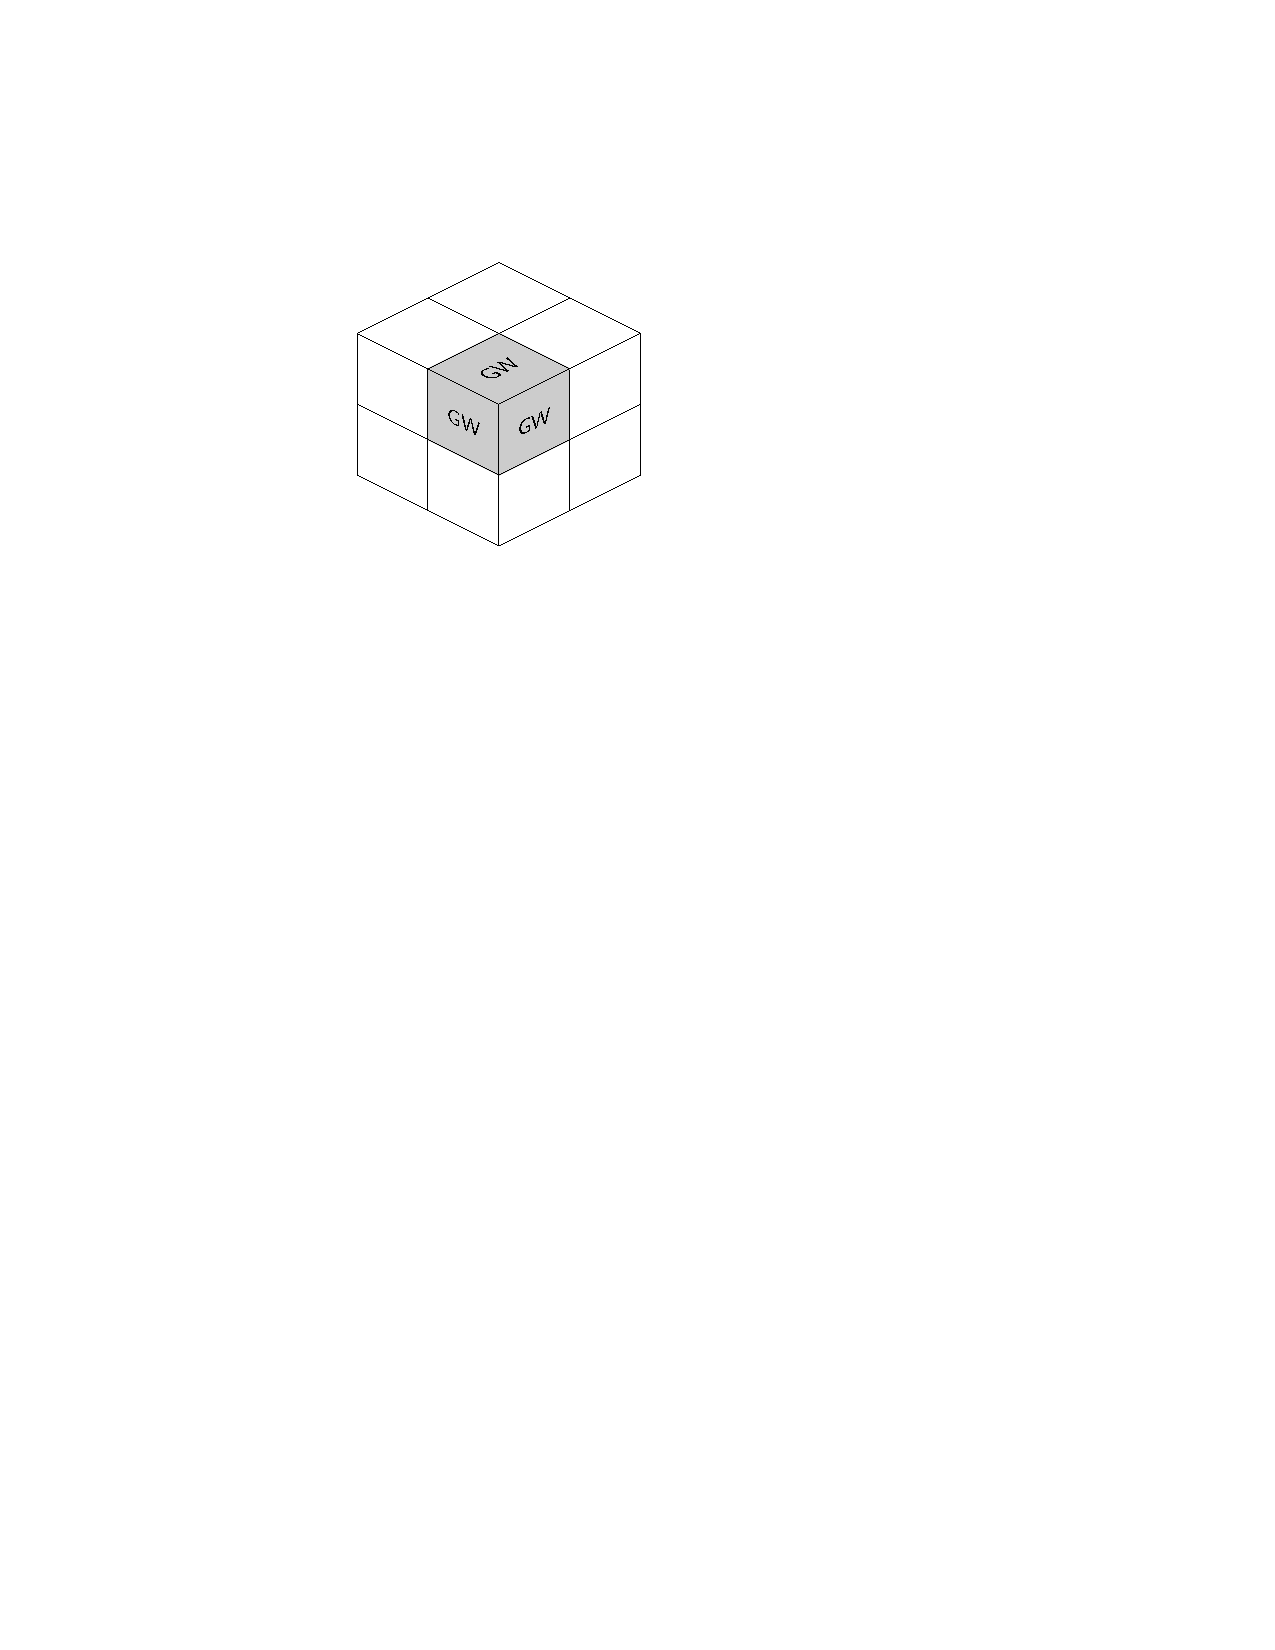
\includegraphics[scale=0.35]{OT_new/cube_gw.pdf}};
\end{tikzpicture}

\vspace{-0.3cm}
\begin{minipage}[t]{0.5\linewidth}
\begin{itemize}
  \item[$\bullet$] Metric properties
  \item[$\bullet$] Isometries.
  \item[$\bullet$] Quadratic and nonconvex problem.
\end{itemize}
\end{minipage}%
\hfill%
\hspace{-6cm}
\begin{minipage}[t]{0.55\linewidth}
  % \vspace{0.1cm}
\begin{figure}
  \centering
  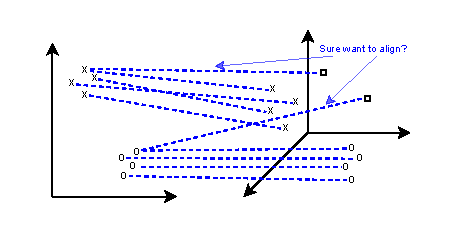
\includegraphics[width=1.2\linewidth, keepaspectratio=true]{OT_new/ugw_transition.pdf}
\end{figure}
\end{minipage}

\end{frame}
%%%%%%%%%%%%%%%%%%%%%%%%%%%%%%%%%%%%%
\begin{frame}{Extension 1: Marginal relaxation}
  \vspace{-0.5cm}
  \scriptsize
  \begin{definition}[Unbalanced GW \parencite{Sejourne20}]
    Given a Csiszár divergence $D_{\varphi}$ and $\lambda_1, \lambda_2 > 0$,
    the unbalanced GW divergence between two compact metric-measure spaces
    $\cX_1 = (X_1, \mu_1, d_1)$ and $\cX_2 = (X_2, \mu_2, d_2)$ is defined as
    \begin{align*}
      \ugw_p^p(\cX_1, \cX_2) = \inf_{\pi \in \cM^+(X_1 \times X_2)} \cL_{\ugw}(\pi),
    \end{align*}
    \vspace{-0.3cm}
    where
    \vspace{-0.5cm}
    \begin{align*}
      \cL_{\ugw}(\pi) &= \iint \left| d_1({\color{blue}{x_1}}, {\color{red}{x_1'}}) - d_2({\color{blue}{x_2}}, {\color{red}{x_2'}}) \right|^p
      \rmd\pi({\color{blue}{x_1, x_2}}) \; \rmd\pi({\color{red}{x_1', x_2'}}) \\
      &+ \lambda_1 D_{\varphi}(\pi_{\# 1} \otimes \pi_{\# 1} | \mu_1 \otimes \mu_1)
      + \lambda_2 D_{\varphi}(\pi_{\# 2} \otimes \pi_{\# 2} | \mu_2 \otimes \mu_2).
    \end{align*}
  \end{definition}

  \vspace{-0.5cm}
  \begin{tikzpicture}[remember picture, overlay]
    \node[shift={(-4cm,-5.5cm)}] at (current page.center)
    {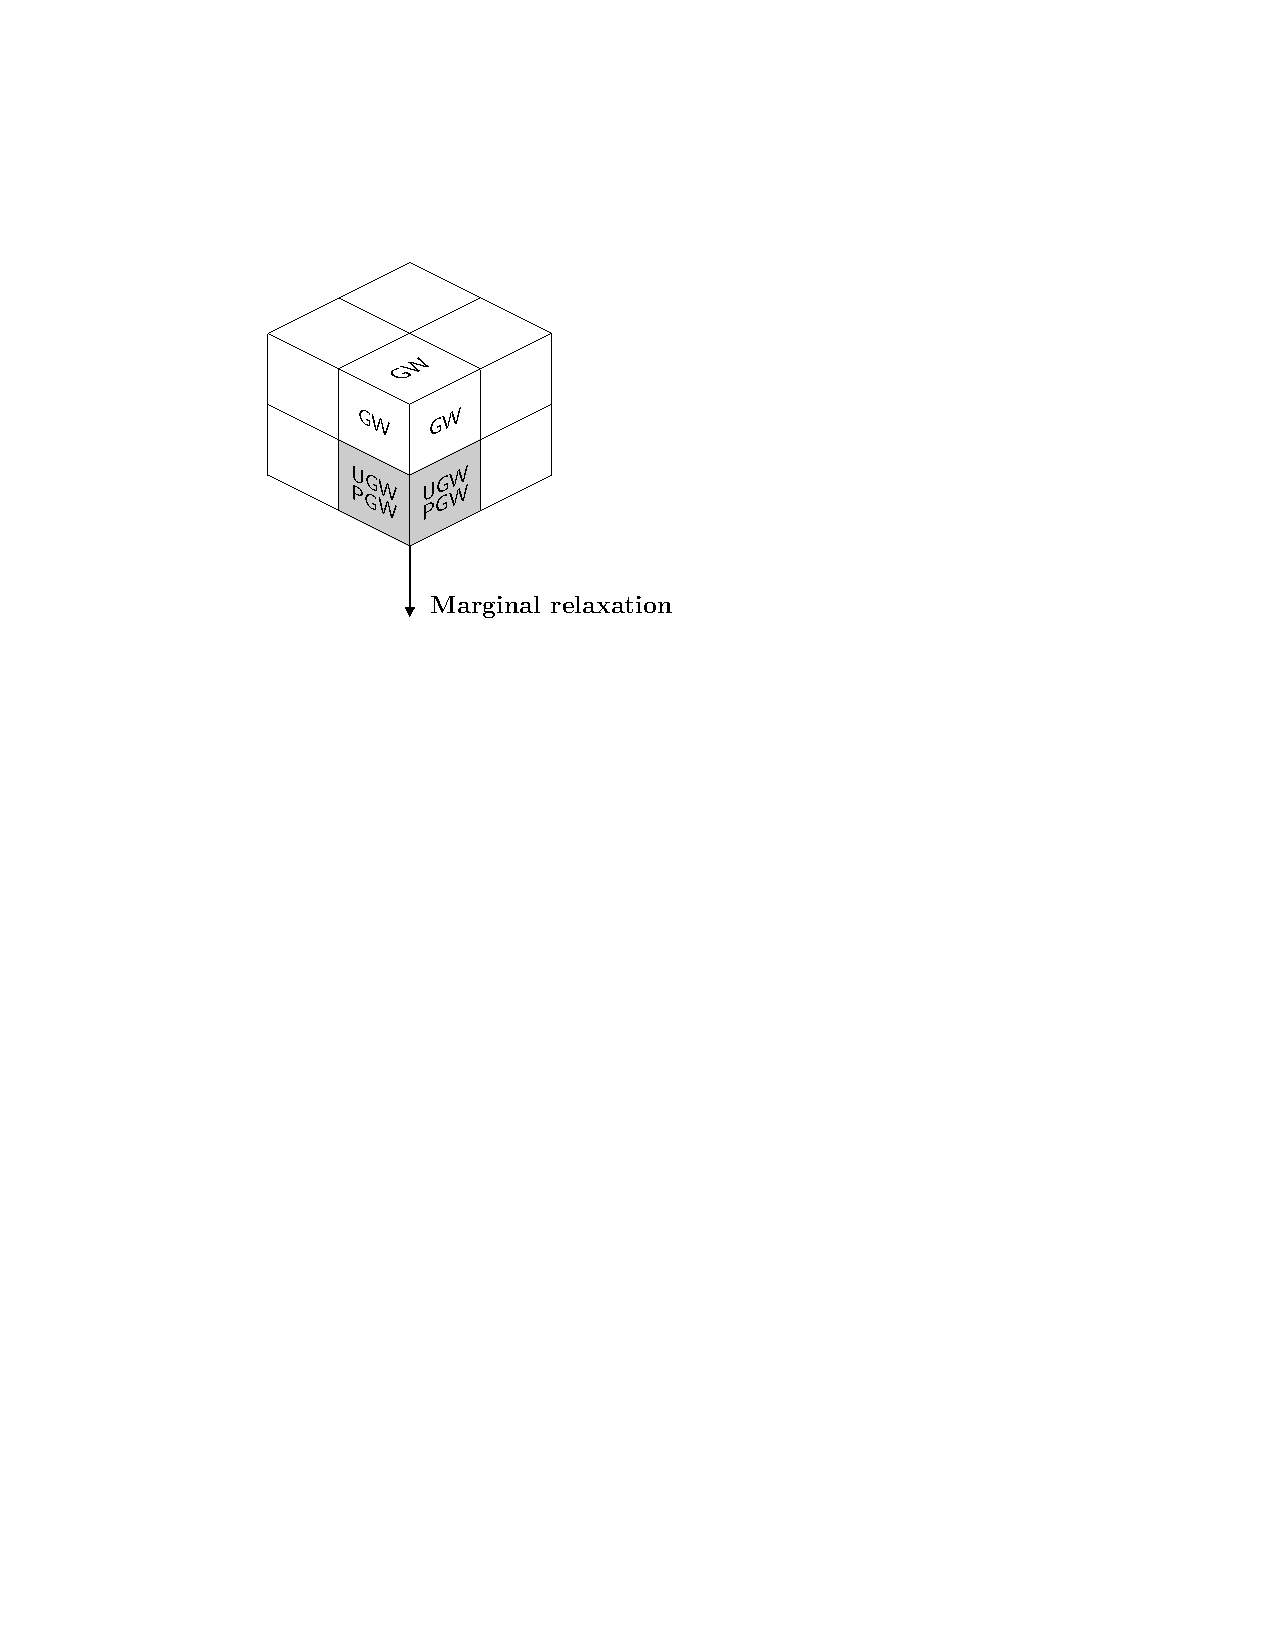
\includegraphics[scale=0.35]{OT_new/cube_ugw.pdf}};
  \end{tikzpicture}

  \begin{minipage}[t]{0.6\linewidth}
  \begin{itemize}
    \item[$\bullet$] Quadratic div: $D_{\varphi}(p \otimes p | q \otimes q) \neq D_{\varphi}(p | q)$.
    \item[$\bullet$] In practice: $D_{\varphi} = \text{Kullback-Leibler div}$.
    \item[$\bullet$] Characterizing isometries.
    \item[$\bullet$] Partial GW \parencite{Chapel20}.
  \end{itemize}
  \end{minipage}%
  \hfill%
  \hspace{-6cm}
  \begin{minipage}[t]{0.45\linewidth}
    \vspace{0.2cm}
  \begin{figure}
    \centering
    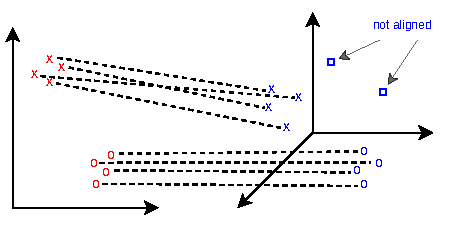
\includegraphics[width=1.15\linewidth, keepaspectratio=true]{OT_new/ugw.pdf}
  \end{figure}
  \end{minipage}

\end{frame}

%%%%%%%%%%%%%%%%%%%%%%%%%%%%%%%%%%%%%
\begin{frame}{Extension 2: Shared subspace (1)}
  \begin{figure}
    \centering
    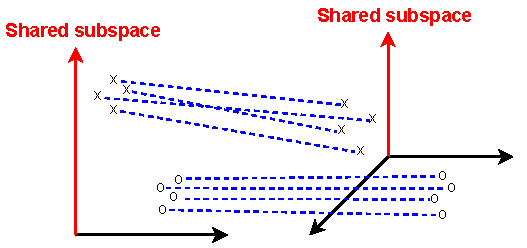
\includegraphics[width=0.8\linewidth, keepaspectratio=true]{OT_new/fgw_abstract.pdf}
  \end{figure}

  \begin{figure}
    \centering
    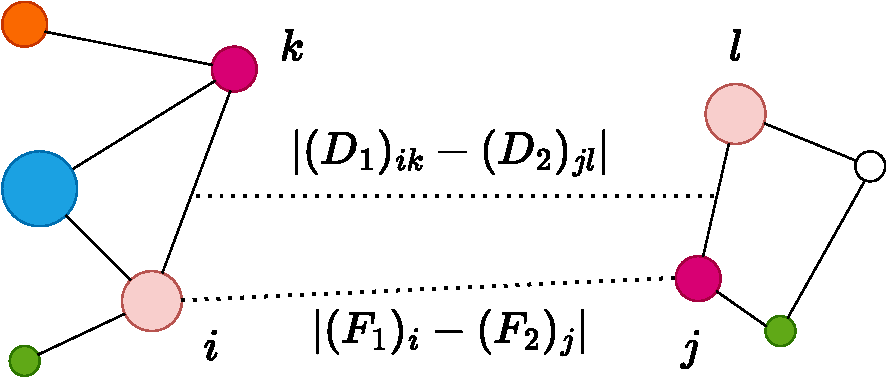
\includegraphics[width=0.8\linewidth, keepaspectratio=true]{OT_new/fgw.pdf}
  \end{figure}

  \begin{tikzpicture}[remember picture, overlay]
    % we don't want to affect the bounding box if the rectangle is too large
    \begin{pgfinterruptboundingbox}
        % the following coords. may need to be changed to suit your slides
        \fill <1> [fill=white, opacity=0.8] (0,0.6) rectangle (10, 4.5);
    \end{pgfinterruptboundingbox}
  \end{tikzpicture}
\end{frame}

%%%%%%%%%%%%%%%%%%%%%%%%%%%%%%%%%%%%%
\begin{frame}{Extension 2: Shared subspace (1)}
  \begin{figure}
    \centering
    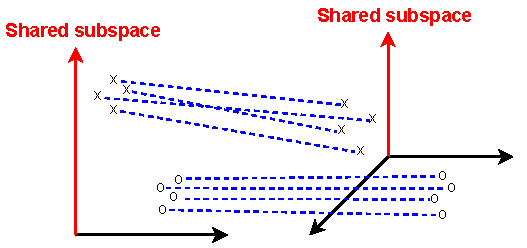
\includegraphics[width=0.8\linewidth, keepaspectratio=true]{OT_new/fgw_abstract.pdf}
  \end{figure}

  \begin{figure}
    \centering
    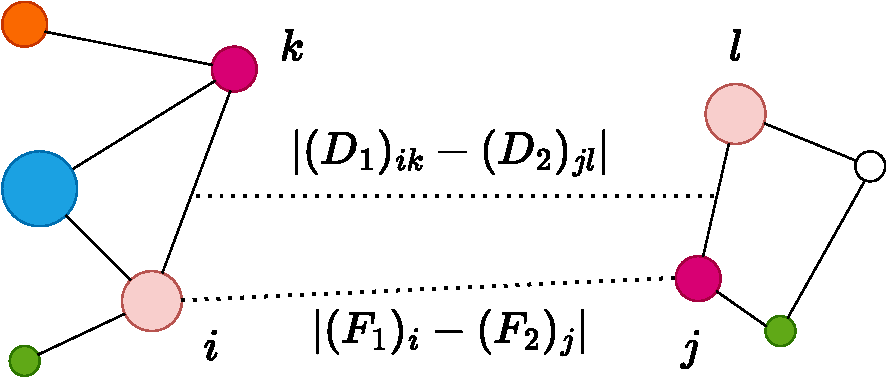
\includegraphics[width=0.8\linewidth, keepaspectratio=true]{OT_new/fgw.pdf}
  \end{figure}
\end{frame}

%%%%%%%%%%%%%%%%%%%%%%%%%%%%%%%%%%%%%
\begin{frame}{Extension 2: Shared subspace (2)}
  \scriptsize
  \vspace{-0.7cm}
  \begin{definition}[Fused GW \parencite{Vayer19b}]
    For $\alpha \in [0, 1]$, the fused GW between two attributed graphs
    $\cX_1 = (D_1, F_1, \mu_1)$ and $\cX_2 = (D_2, F_2, \mu_2)$,
    where $D_k \in \bbR^{n_k \times n_k}, F_k \in \bbR^{n_k \times d}$
    and $\mu_k \in \Delta_{n_k}$, is defined as
    \begin{align*}
      \fgw_p^p(\cX_1, \cX_2) = \inf_{\pi \in U(\mu_1, \mu_2)} \cL_{\fgw}(\pi),
    \end{align*}
    \vspace{-0.3cm}
    where
    \begin{align*}
      \cL_{\fgw}(\pi) = (1 - \alpha)
      \sum_{{\color{blue}{i}},{\color{blue}{j}},{\color{red}{k}},{\color{red}{l}}}
      |(D_1)_{{\color{blue}{i}} {\color{red}{k}}} - (D_2)_{{\color{blue}{j}}{\color{red}{l}}}|^p \pi_{\color{blue}{{ij}}} \pi_{\color{red}{{kl}}}
      + \alpha \sum_{{\color{blue}{i,j}}} ||(F_1)_{\color{blue}{i}} - (F_2)_{\color{blue}{j}}||^q \pi_{\color{blue}{{ij}}}.
    \end{align*}
  \end{definition}

  \begin{tikzpicture}[remember picture, overlay]
    \node[shift={(-4cm,-5.5cm)}] at (current page.center)
    {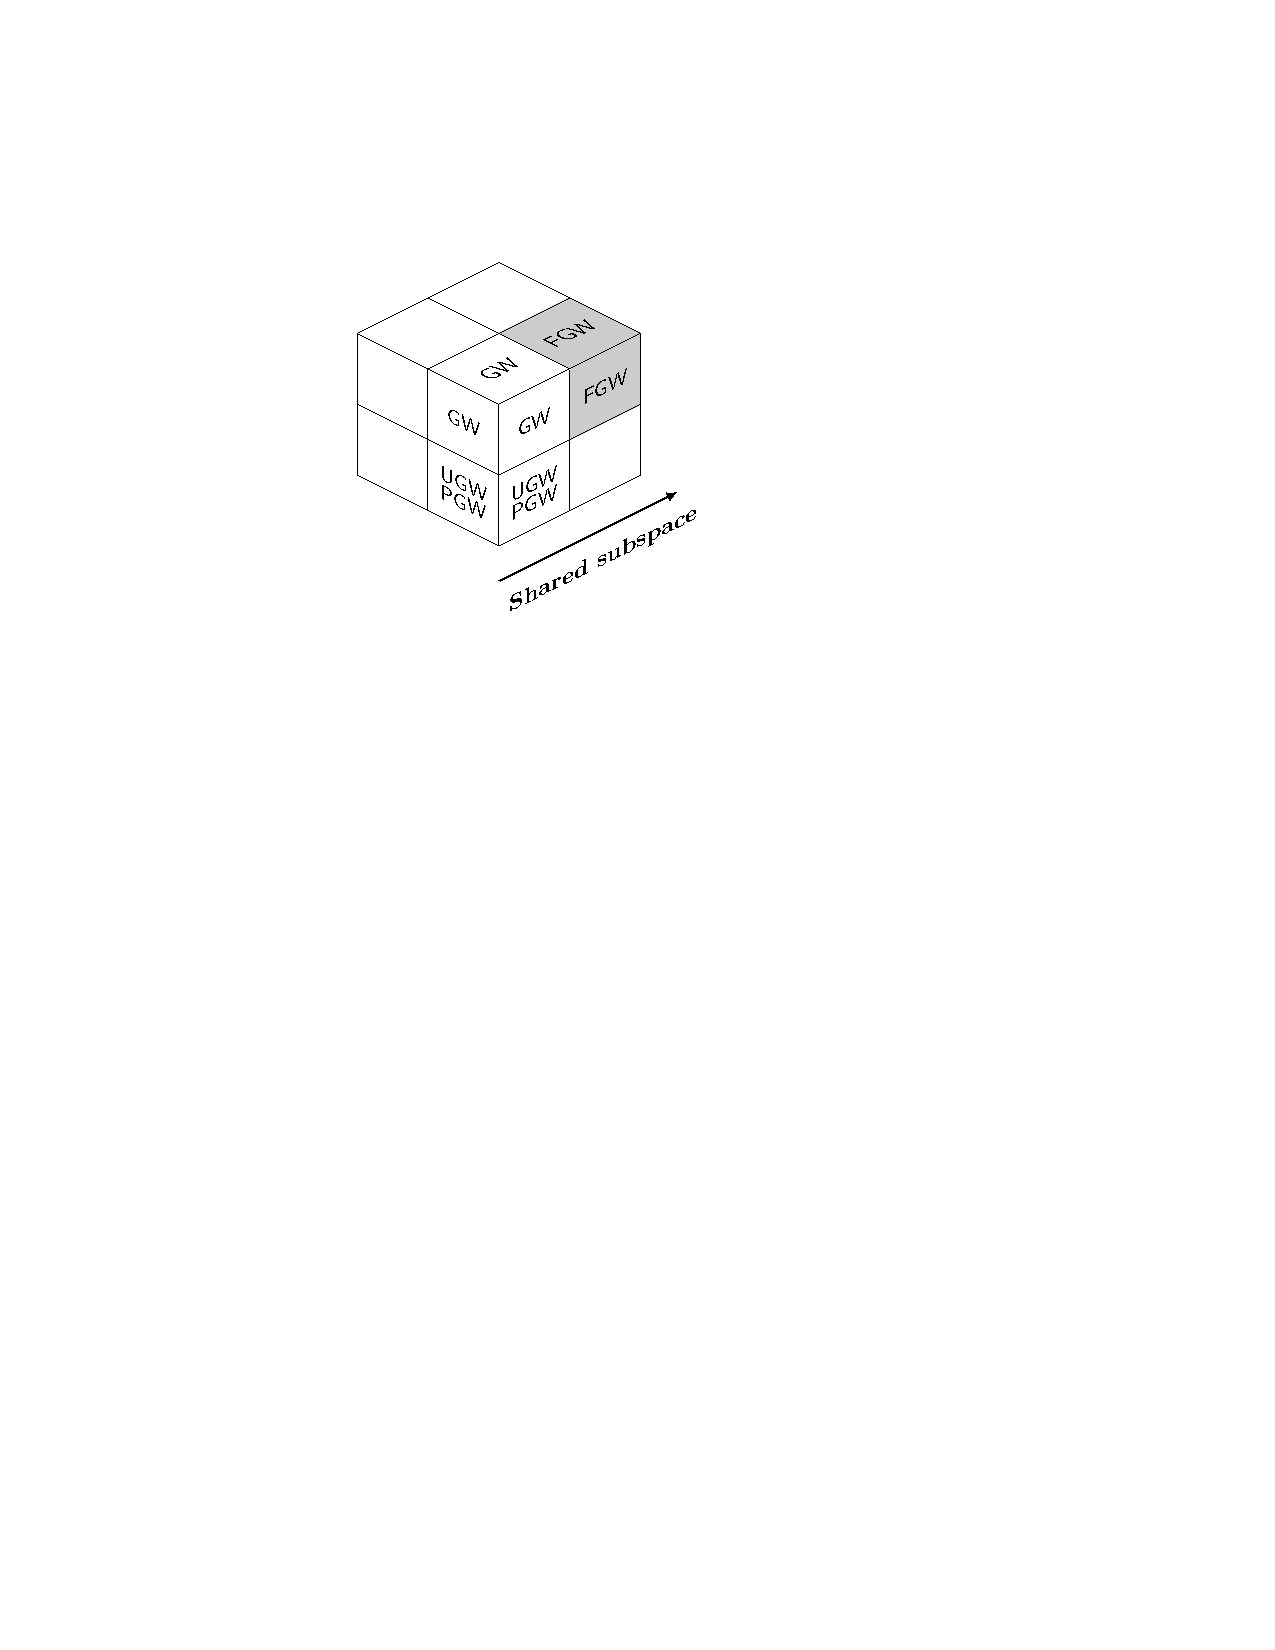
\includegraphics[scale=0.35]{OT_new/cube_fgw.pdf}};
  \end{tikzpicture}

  \vspace{-0.3cm}
  \begin{minipage}[t]{0.6\linewidth}
    \begin{itemize}
      \item[$\bullet$] Interpolation between GW and Wasserstein.
      \item[$\bullet$] Feature-preserving isometries.
    \end{itemize}
    \end{minipage}%
    \hfill%
    \hspace{-6cm}
    \begin{minipage}[t]{0.45\linewidth}
      \vspace{-0.cm}
    \begin{figure}
      \centering
      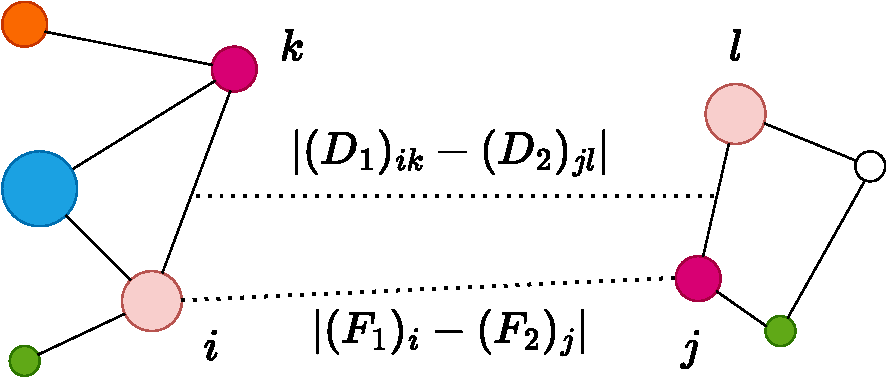
\includegraphics[width=1.1\linewidth, keepaspectratio=true]{OT_new/fgw.pdf}
      % \caption*{\scriptsize{Inspired by \parencite{Vayer19b}}}
    \end{figure}
    \end{minipage}

\end{frame}

%%%%%%%%%%%%%%%%%%%%%%%%%%%%%%%%%%%%%%%%%%%%%%%
\begin{frame}{Extension 2: Shared subspace (2)}
  \begin{figure}
    \centering
    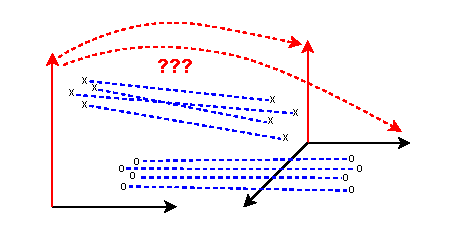
\includegraphics[width=\linewidth, keepaspectratio=true]{OT_new/coot_motiv.pdf}
  \end{figure}
\end{frame}

%%%%%%%%%%%%%%%%%%%%%%%%%%%%%%%%%%%%%
\begin{frame}{Extension 3: Bilinear relaxation (1)}
  \begin{figure}
    \centering
    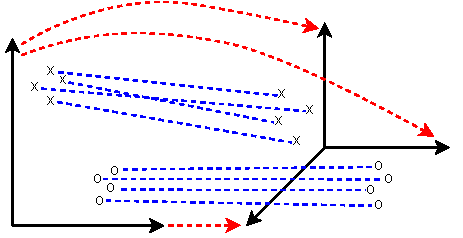
\includegraphics[width=0.7\linewidth, keepaspectratio=true]{OT_new/coot_new.pdf}
  \end{figure}

  \begin{figure}
    \centering
    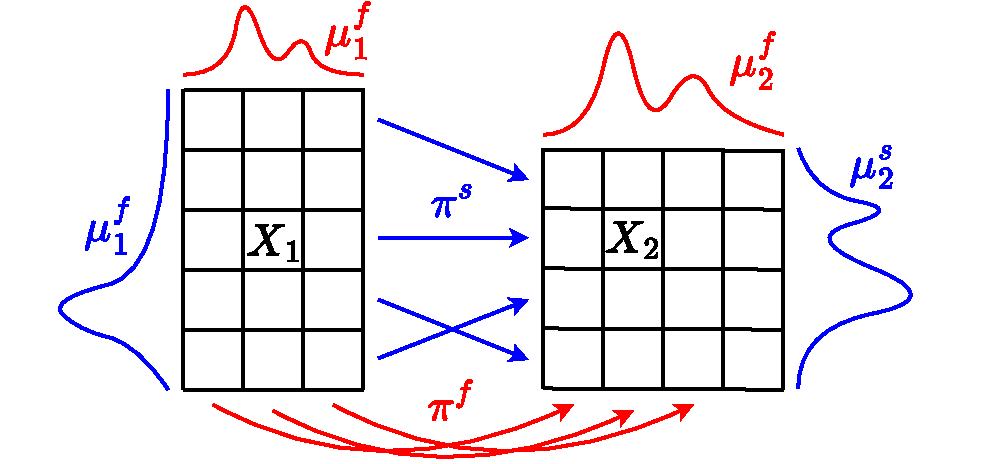
\includegraphics[width=0.7\linewidth, keepaspectratio=true]{OT_new/coot_matrix_ot.pdf}
    \caption*{\scriptsize{{\color{blue}{Sample}} and {\color{red}{feature}} transport plans in discrete setting.}}
  \end{figure}

  \begin{tikzpicture}[remember picture, overlay]
    % we don't want to affect the bounding box if the rectangle is too large
    \begin{pgfinterruptboundingbox}
        % the following coords. may need to be changed to suit your slides
        \fill <1> [fill=white, opacity=0.8] (0,0) rectangle (12, 5);
    \end{pgfinterruptboundingbox}
  \end{tikzpicture}
\end{frame}

%%%%%%%%%%%%%%%%%%%%%%%%%%%%%%%%%%%%%
\begin{frame}{Extension 3: Bilinear relaxation (1)}
  \begin{figure}
    \centering
    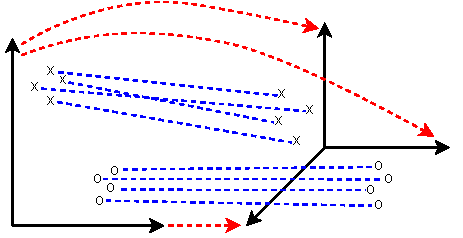
\includegraphics[width=0.7\linewidth, keepaspectratio=true]{OT_new/coot_new.pdf}
  \end{figure}

  \begin{figure}
    \centering
    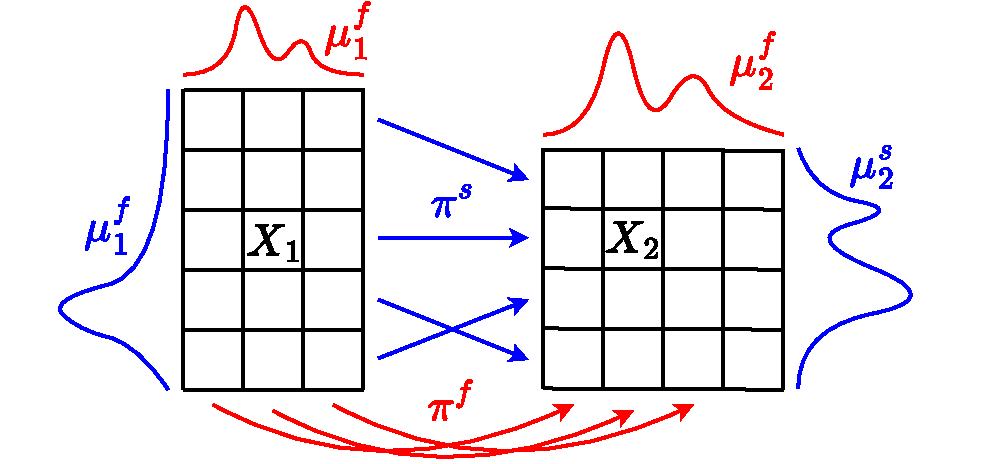
\includegraphics[width=0.7\linewidth, keepaspectratio=true]{OT_new/coot_matrix_ot.pdf}
    \caption*{\scriptsize{{\color{blue}{Sample}} and {\color{red}{feature}} transport plans in discrete setting.}}
  \end{figure}
\end{frame}

%%%%%%%%%%%%%%%%%%%%%%%%%%%%%%%%%%%%%%%%%%%%%%%%%%%%%%
\begin{frame}{Extension 3: Bilinear relaxation (2)}
\scriptsize
\vspace{-0.8cm}
\begin{definition}[Discrete COOT \parencite{Redko20}]
  The Co-Optimal Transport distance between
  two weighted matrices $\cX_1 = (X_1, \mssrc, \mfsrc)$
and $\cX_2 = (X_2, \mstg, \mftg)$, where
$X_k \in \bbR^{n_k \times d_k}$ and histograms
${\color{blue}{\mu^s_k \in \Delta_{n_k}}}, {\color{red}{\mu^f_k \in \Delta_{d_k}}}$,
is defined as
\begin{align*}
  \coot_p^p(\cX_1, \cX_2) =
  \min_{\substack{\pis \in U(\mssrc,\mstg) \\ \pif \in U(\mfsrc,\mftg)}}
  \sum_{{\color{blue}{i}},{\color{blue}{j}},{\color{red}{k}},{\color{red}{l}}}
  |(X_1)_{{\color{blue}{i}} {\color{red}{k}}} - (X_2)_{{\color{blue}{j}}{\color{red}{l}}}|^p {\color{blue}{\pi^s_{ij}}} {\color{red}{\pi^f_{kl}}}
\end{align*}
\end{definition}

\begin{tikzpicture}[remember picture, overlay]
  \node[shift={(-4cm,-5.5cm)}] at (current page.center)
  {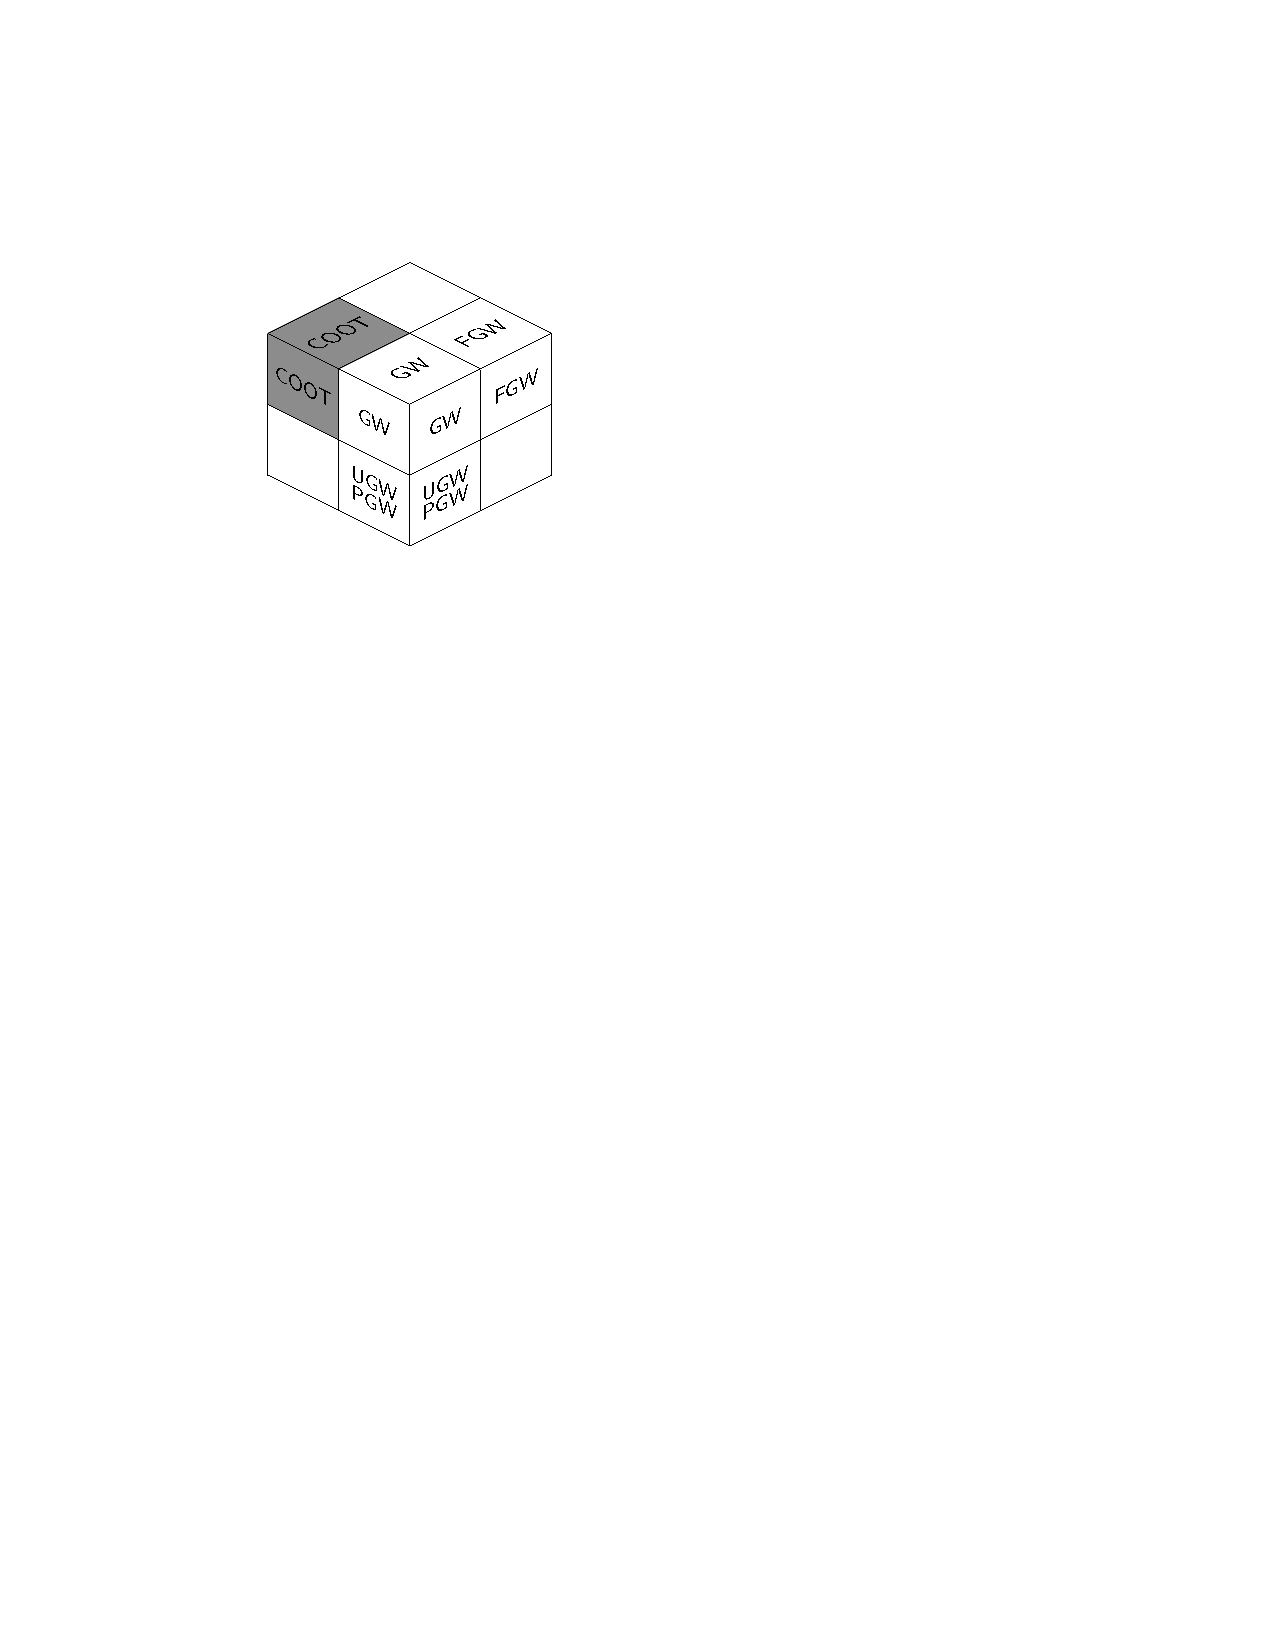
\includegraphics[scale=0.35]{OT_new/cube_coot.pdf}};
\end{tikzpicture}

\vspace{-0.5cm}
\begin{minipage}[t]{0.6\linewidth}
  \begin{itemize}
    \item[$\bullet$] Continuous extension \parencite{Chowdhury21b}.
    \item[$\bullet$] Comparing \underline{arbitrary-size} matrices.
    \item[$\bullet$] {\color{red}{Feature}} coupling:
    \begin{enumerate}
      \scriptsize
      \setlength\itemindent{10pt}
      \item[1.] Is meaningful.
      \item[2.] Improves {\color{blue}{sample}} alignments.
    \end{enumerate}
    \item[$\bullet$] Connection with GW distance.
  \end{itemize}
  \end{minipage}%
  \hfill%
  \hspace{-6cm}
  \begin{minipage}[t]{0.55\linewidth}
    \vspace{0.2cm}
  \begin{figure}
    \centering
    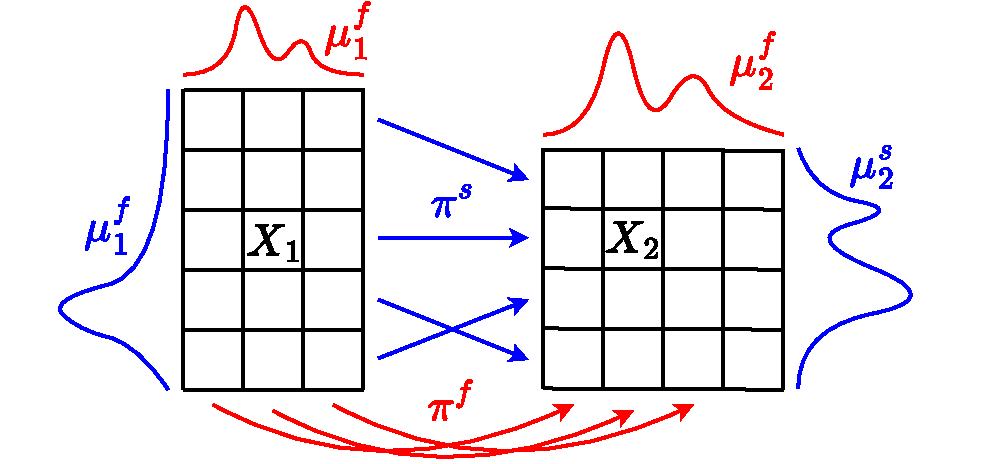
\includegraphics[width=1.2\linewidth, keepaspectratio=true]{OT_new/coot_matrix_ot.pdf}
  \end{figure}
\end{minipage}

\end{frame}

%%%%%%%%%%%%%%%%%%%%%%%%%%%%%%%%%%%%%%%%%%%
\begin{frame}{Contributions of the thesis}
  \begin{tikzpicture}[remember picture, overlay]
    \node[shift={(0cm,-4cm)}] at (current page.center)
    {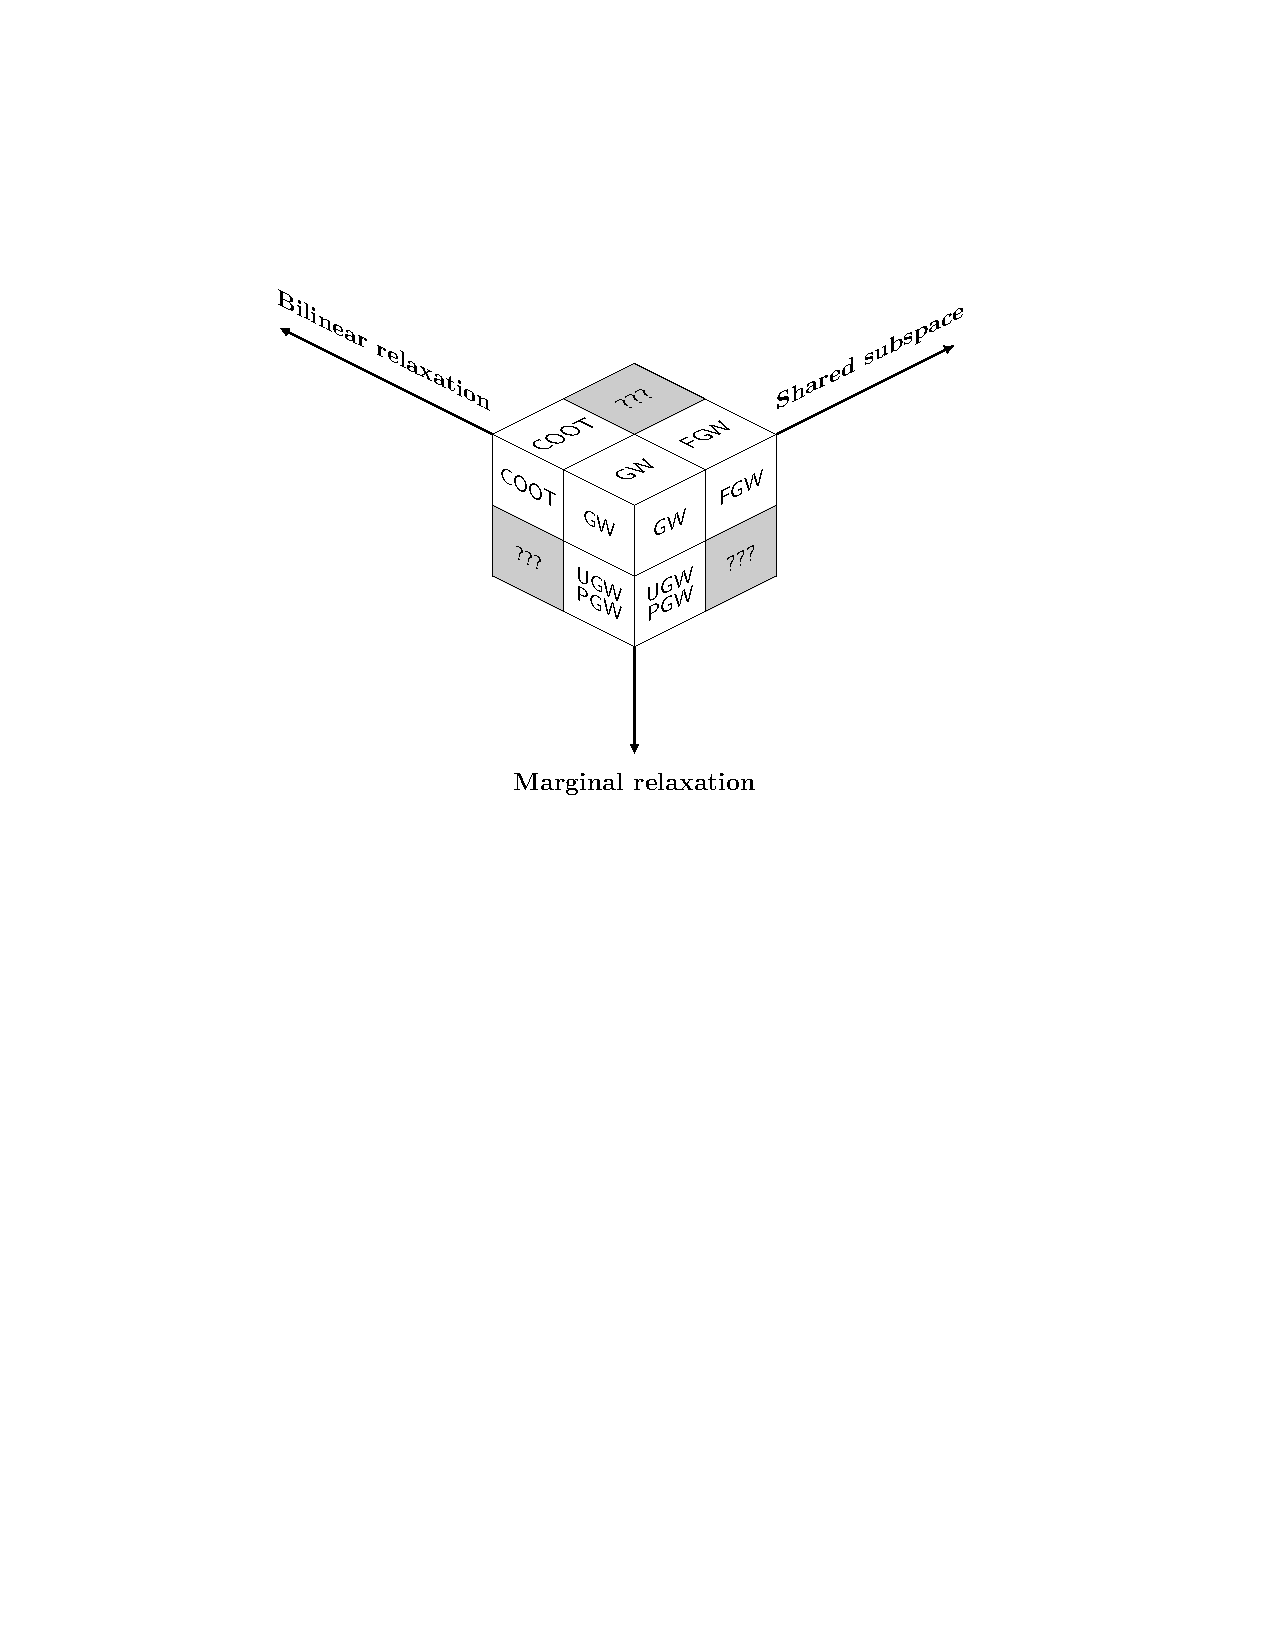
\includegraphics[scale=0.8]{OT_new/cube_intro.pdf}};
  \end{tikzpicture}
\end{frame}

%%%%%%%%%%%%%%%%%%%%%%%%%%%%%%%%%%%%%%%%
%%%%%%%%%%%%%%%%%%%%%%%%%%%%%%%%%%%%%%%%
%%%% Contribution on FUGW
\section{Fused Unbalanced Gromov-Wasserstein}

%%%%%%%%%%%%%%%%%%%%%%%%%%%%%%%%%%%%%%%%%%%%
\begin{frame}{Motivation from neuroscience}
\scriptsize
\begin{itemize}
  \setlength\itemsep{0.3cm}
  \item[$\bullet$] High variability in human anatomies and functional MRI responses across subjects.

  $\Rightarrow$ Allow for adaptation of inter-individual variability.

  \item[$\bullet$] Averaging functional surface brains results in loss of individual details.

  $\Rightarrow$ Generate sharper barycenters for functional signals.

  \item[$\bullet$] Lack of efficient methods for brain alignments.

  $\Rightarrow$ Exploit anatomical and functional information.
\end{itemize}
\begin{figure}
  \centering
  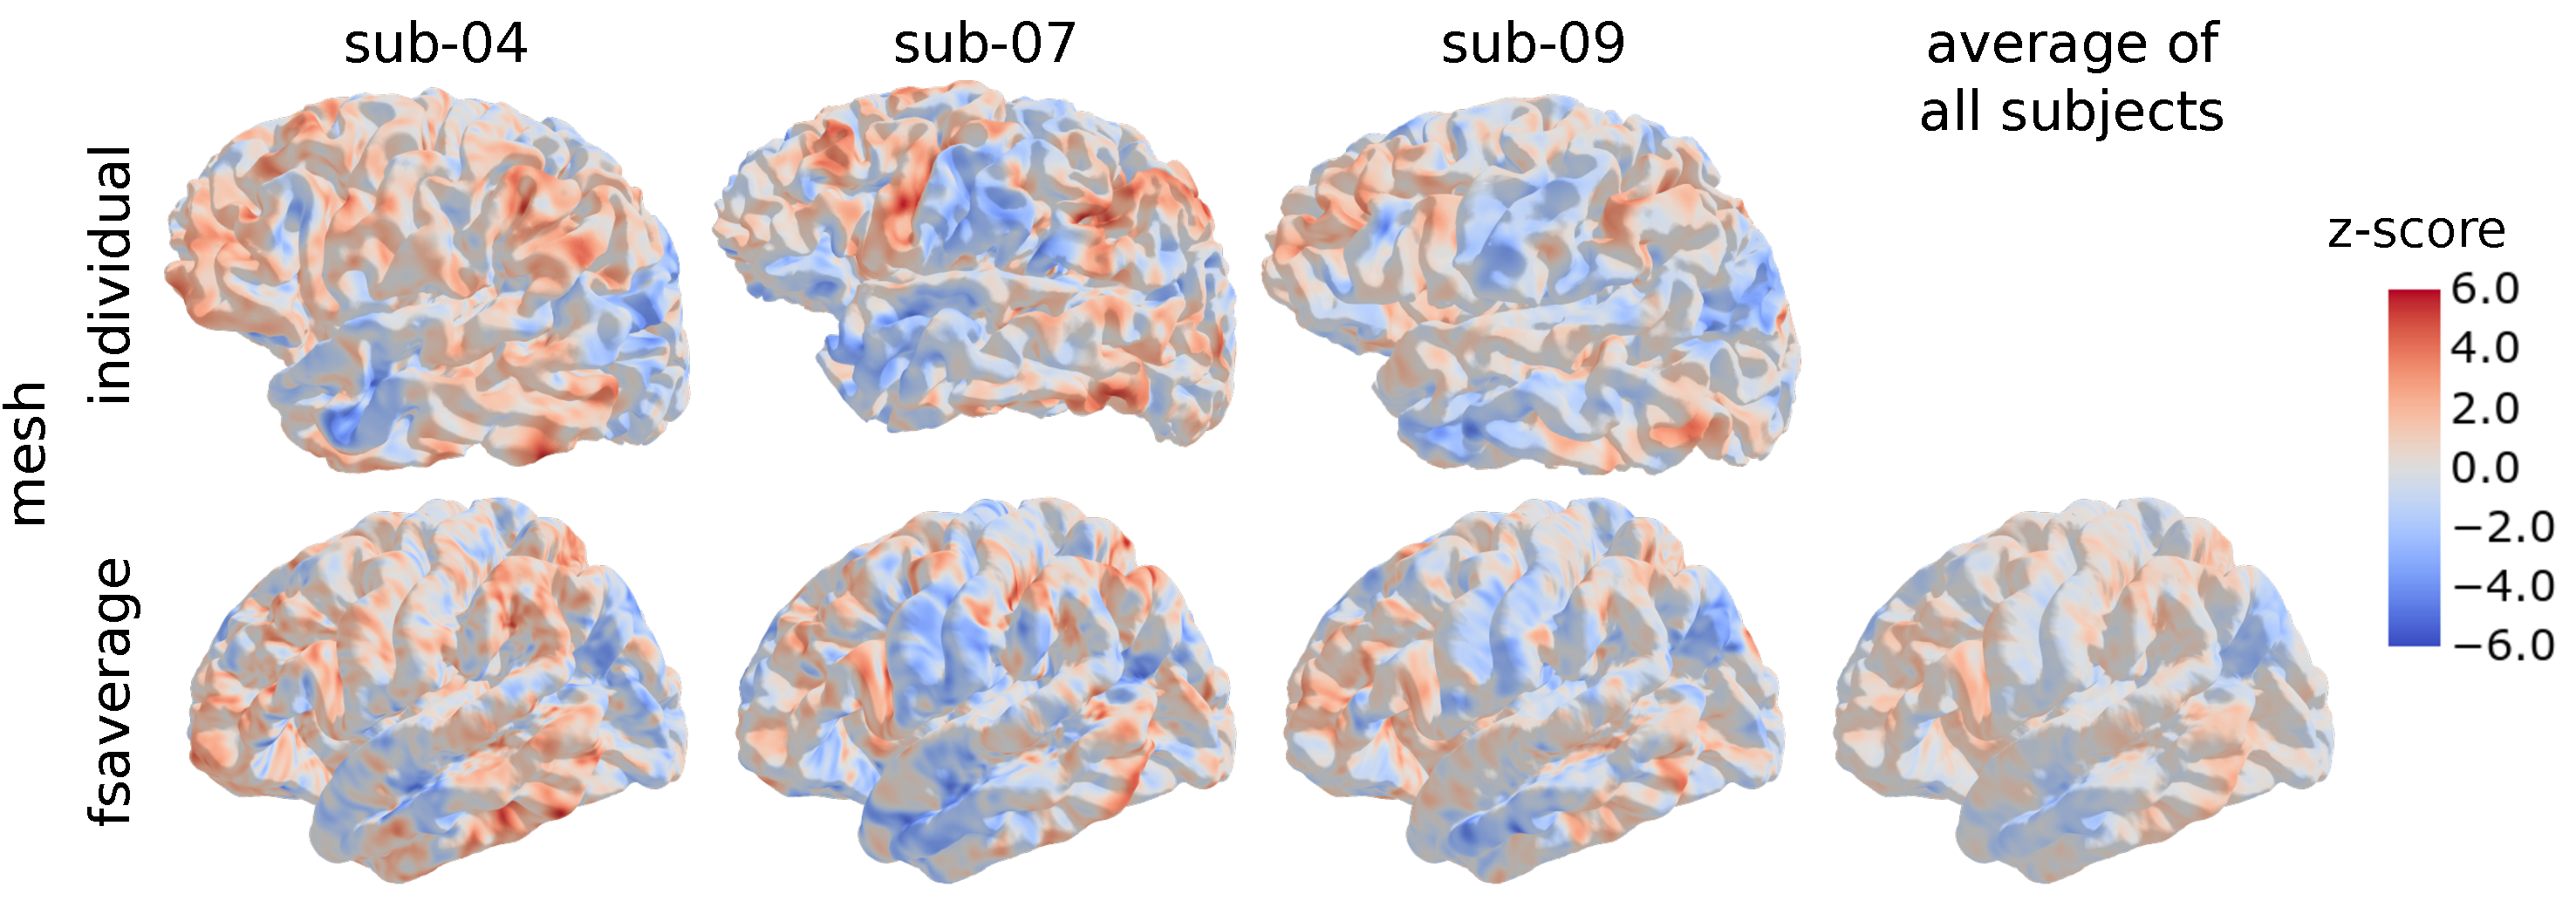
\includegraphics[width=1.\linewidth, keepaspectratio=true]{OT_new/intro_variation.pdf}
  % \caption*{\scriptsize{High variability in human anatomies and functional MRI responses across subjects.}}
\end{figure}
\end{frame}

%%%%%%%%%%%%%%%%%%%%%%%%%%%%%%%%%%%%%%%%%%%
\begin{frame}{Fused Unbalanced Gromov-Wasserstein}
  \scriptsize

  \begin{tikzpicture}[remember picture, overlay]
    \node[shift={(0cm,-1.5cm)}] at (current page.center)
    {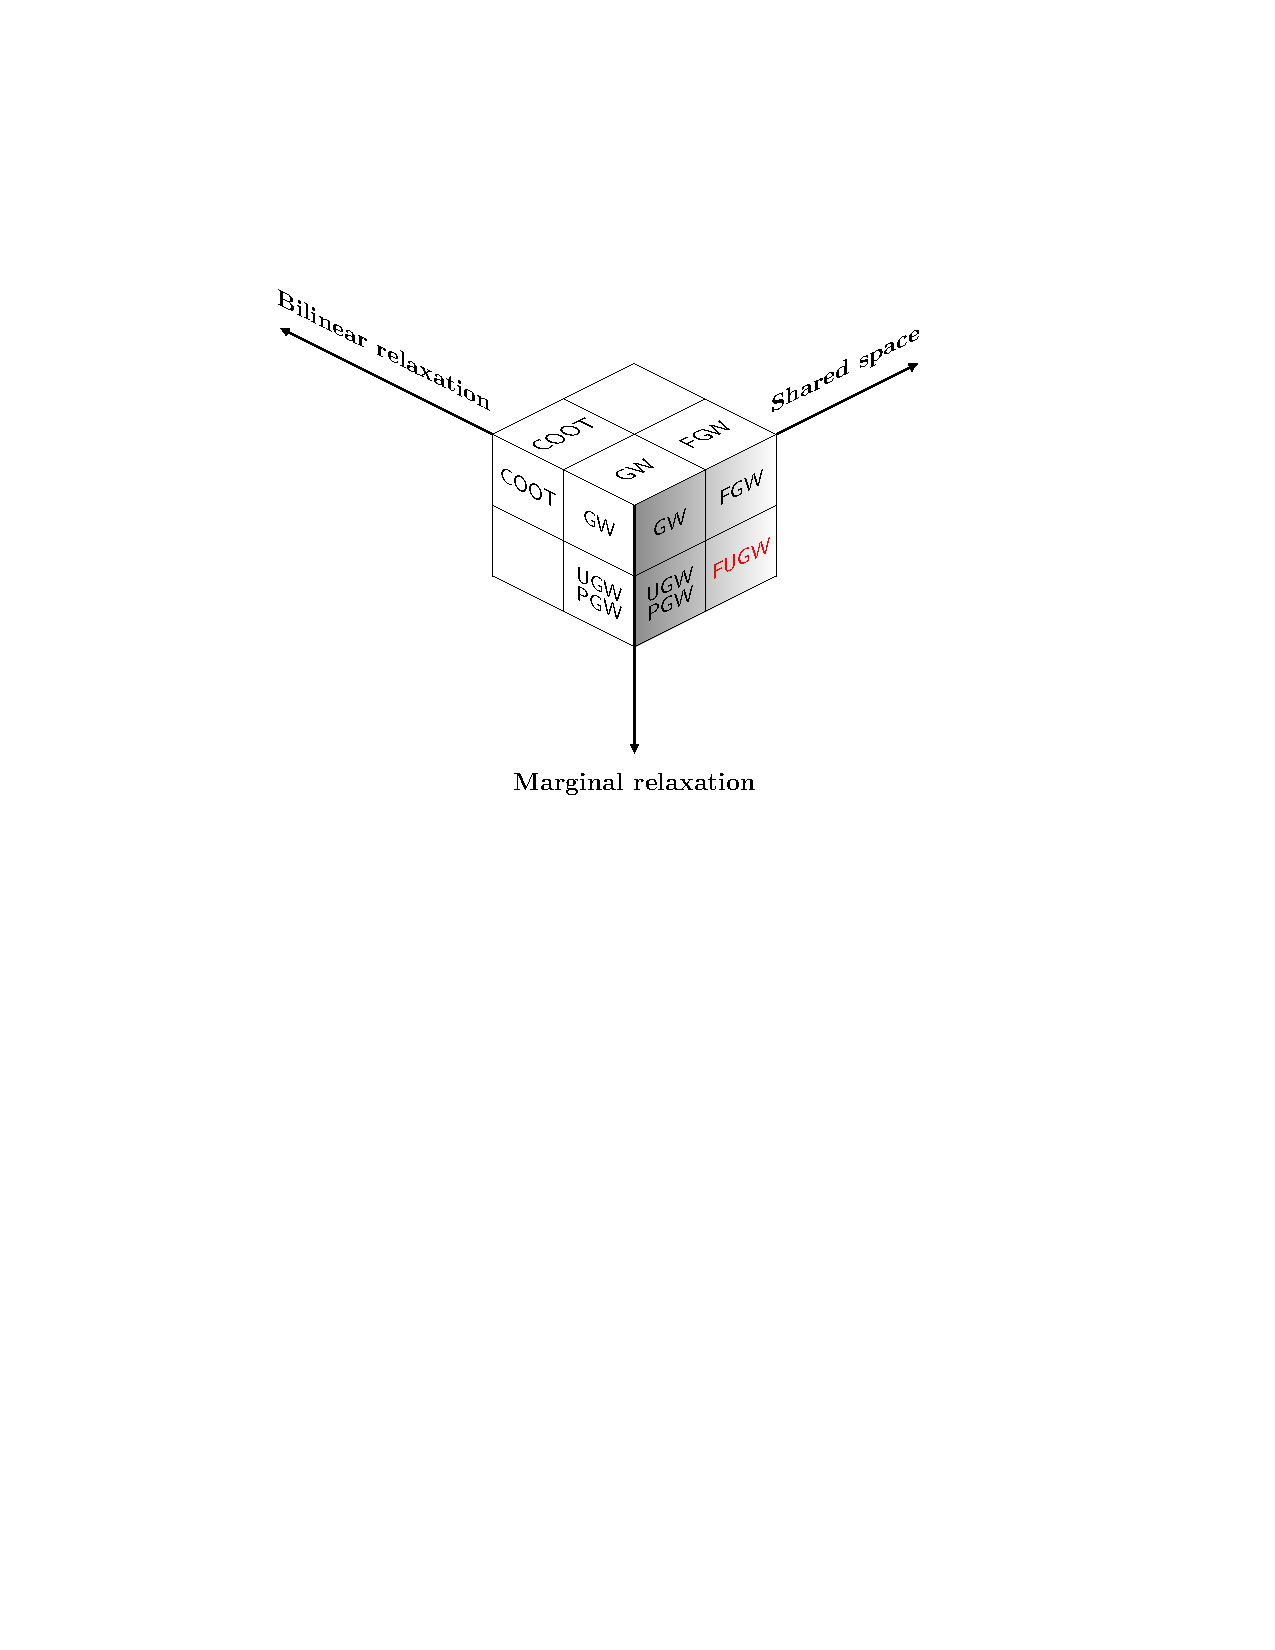
\includegraphics[scale=0.55]{OT_new/cube_fugw_contrib.pdf}};
  \end{tikzpicture}

  \vspace{5cm}
  {\color{brown}{\textbf{Summary}}}: applied fused unbalanced GW to
  \begin{enumerate}
    \setlength\itemindent{10pt}
    \item[1.] Align human cortical surfaces.
    \item[2.] Learn human brain templates.
  \end{enumerate}

  \vspace{0.3cm}
  {\color{brown}{\textbf{Publication}}}: Aligning individual brains with Fused Unbalanced Gromov-Wasserstein.
  Alexis Thual*, QHT*, Tatiana Zemskova, Nicolas Courty,
  Rémi Flamary, Stanislas Dehaene, and Bertrand Thirion.
  Advances in neural information processing systems (NeurIPS), 2022.

\end{frame}

%%%%%%%%%%%%%%%%%%%%%%%%%%%%%%%%%%%%%%%%%%%%
\begin{frame}{Formulation}
\scriptsize
\vspace{-0.7cm}
\begin{block}{Definition}
  Given $\lambda > 0$ and $\alpha \in [0, 1]$, the fused unbalanced GW
  between two attributed graphs $\cX^s = (D^s, F^s, \mu^s)$ and
  $\cX^t = (D^t, F^t, \mu^t)$ is defined as
\begin{align*}
  \fugw(\cX^s, \cX^t) = \inf_{P \in \bbR^{m \times n}_{\geq 0}} \quad
  &(1 - \alpha) \sum_{{\color{blue}{i, j}},{\color{red}{k, l}}} |
  D^s_{{\color{blue}{i}}{\color{red}{k}}} - D^t_{{\color{blue}{j}}{\color{red}{l}}}|^2
  P_{\color{blue}{ij}} P_{\color{red}{kl}}
  + \alpha \sum_{{\color{blue}{i, j}}} || F^s_{\color{blue}{i}} - F^t_{\color{blue}{j}}||_2^2 P_{\color{blue}{ij}} \\
  &+ \lambda \Big[ \kl(P_{\# 1} \otimes P_{\# 1} \vert w^s \otimes w^s)
  + \kl(P_{\# 2} \otimes P_{\# 2} \vert w^t \otimes w^t) \Big].
\end{align*}
\end{block}

\begin{tikzpicture}[remember picture, overlay]
  \node[shift={(-3.7cm,-6.3cm)}] at (current page.center)
  {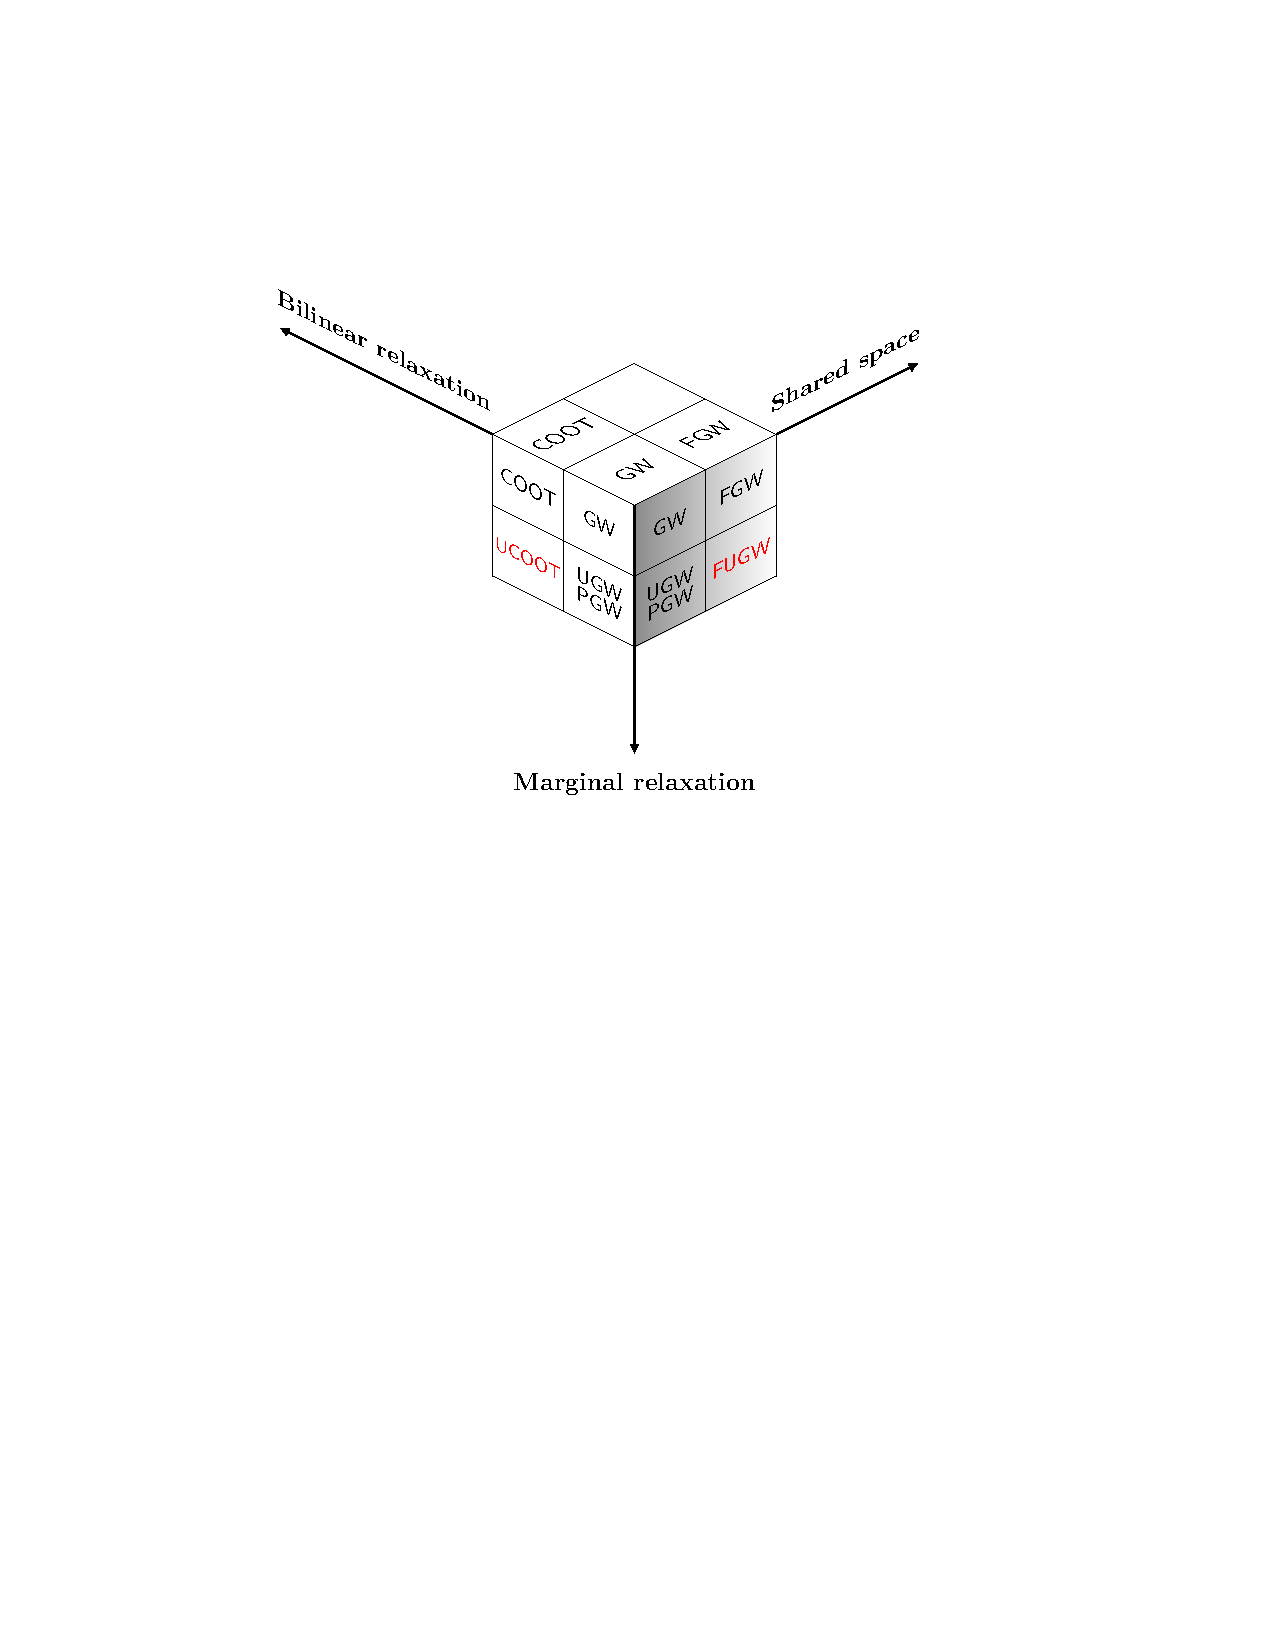
\includegraphics[scale=0.35]{OT_new/cube_fugw.pdf}};
\end{tikzpicture}

\vspace{-0.5cm}
\begin{figure}
  \centering
  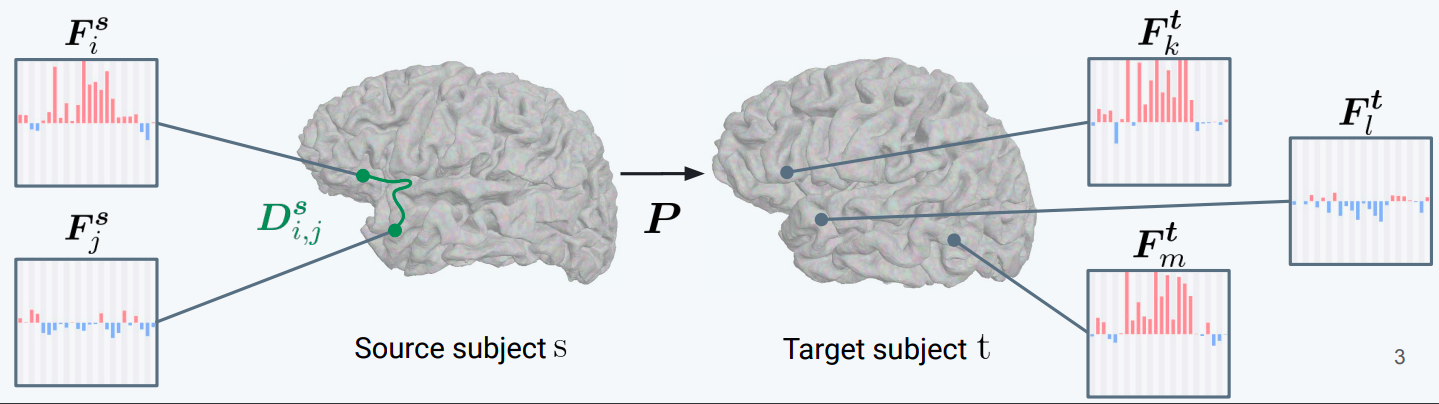
\includegraphics[width=1.\linewidth, keepaspectratio=true]{OT_new/fugw.png}
  \caption*{\scriptsize{Illustration of FUGW on human cortical surfaces}}
\end{figure}
\end{frame}

%%%%%%%%%%%%%%%%%%%%%%%%%%%%%
\begin{frame}{Why is unbalancing important?}
\scriptsize
% \vspace{-0.5cm}
\begin{itemize}
  \item[$\bullet$] Feature = scalar.
  \item[$\bullet$] Source mesh: the signal is constituted of two von Mises
  density functions that differ by their concentration (large and small).
  \item[$\bullet$] Target mesh: only the large one is present, but at a different location.
\end{itemize}
\vspace{0.2cm}
\begin{figure}
  \centering
  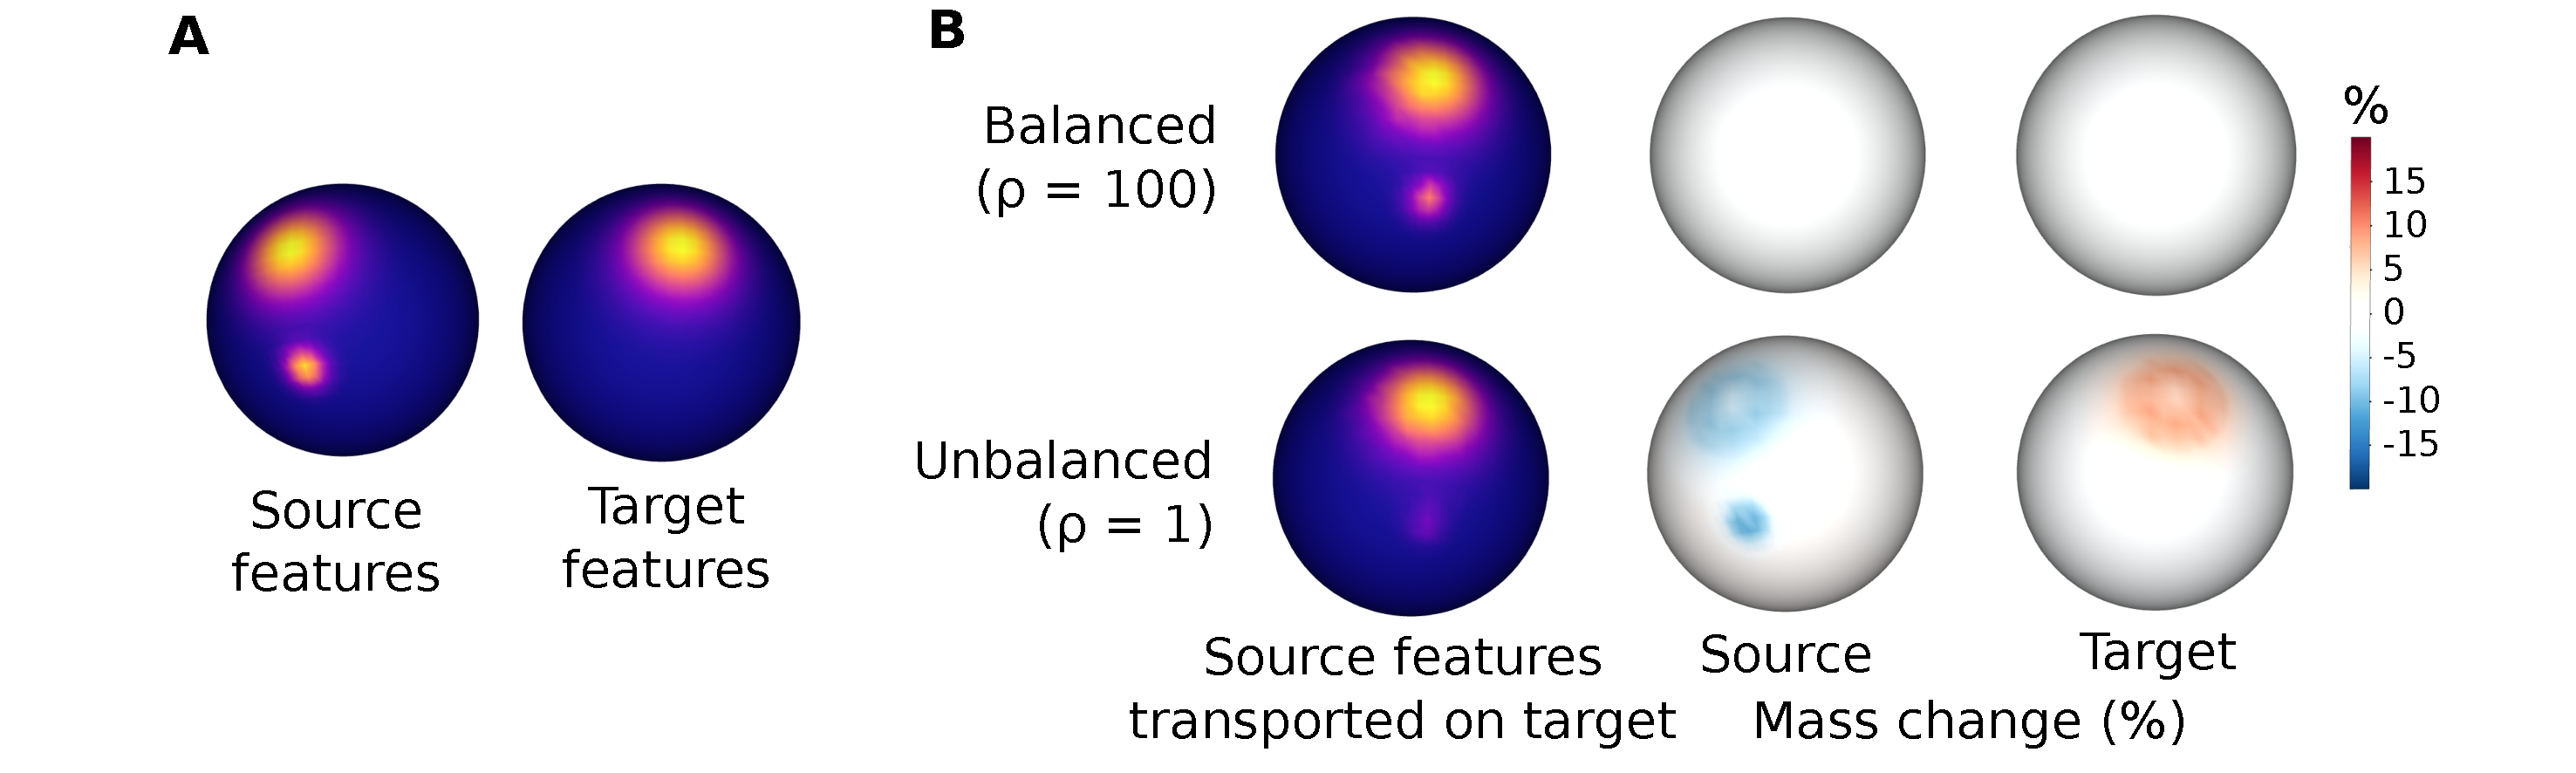
\includegraphics[width=1.\linewidth, keepaspectratio=true]{OT_new/toy_example.pdf}
  \caption*{\scriptsize{Unbalancing helps accounting for idiosyncrasies of the source and target signals.}}
\end{figure}

\begin{tikzpicture}[remember picture, overlay]
  \node[shift={(-3.7cm,-6.3cm)}] at (current page.center)
  {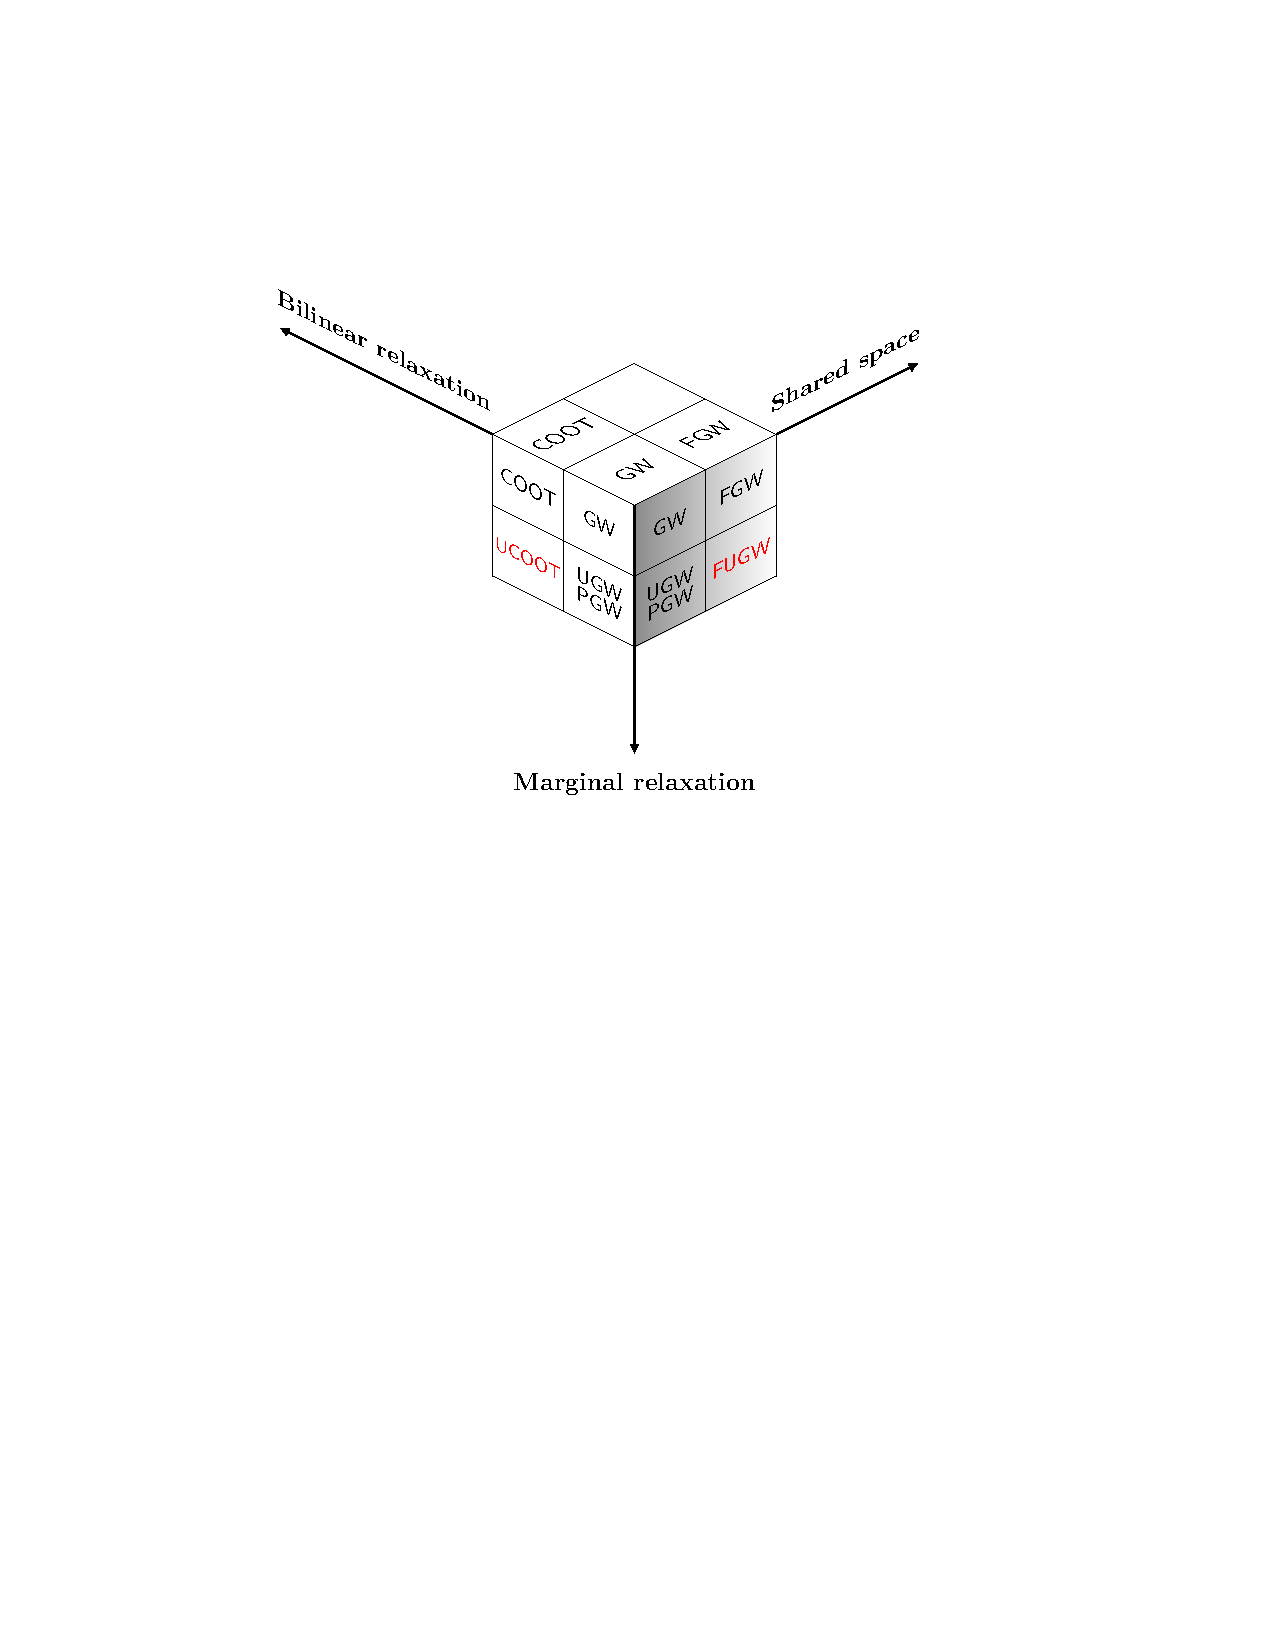
\includegraphics[scale=0.35]{OT_new/cube_fugw.pdf}};
\end{tikzpicture}

\end{frame}

%%%%%%%%%%%%%%%%%%%%%%%%%%%%%
\begin{frame}{Optimization}
\scriptsize
\vspace{-1.3cm}
\begin{align*}
  \cL_{\fugw}({\color{blue}{P}}, {\color{red}{Q}}) &=
  (1 - \alpha) \sum_{{\color{blue}{i, j}},{\color{red}{k, l}}} |
  D^s_{{\color{blue}{i}}{\color{red}{k}}} - D^t_{{\color{blue}{j}}{\color{red}{l}}}|^2
  {\color{blue}{P_{ij}}} {\color{red}{Q_{kl}}} \\
  &+ \frac{\alpha}{2} \sum_{{\color{blue}{i, j}}} || F^s_{\color{blue}{i}} - F^t_{\color{blue}{j}}||_2^2 {\color{blue}{P_{ij}}}
  + \frac{\alpha}{2} \sum_{{\color{red}{k, l}}} || F^s_{{\color{red}{k}}} - F^t_{{\color{red}{l}}}||_2^2 {\color{red}{Q_{kl}}} \\
  &+ \lambda \Big[ \kl({\color{blue}{P}}_{\# 1} \otimes {\color{red}{Q}}_{\# 1} \vert w^s \otimes w^s)
  + \kl({\color{blue}{P}}_{\# 2} \otimes {\color{red}{Q}}_{\# 2} \vert w^t \otimes w^t) \Big].
\end{align*}
\vspace{-0.7cm}
\begin{align*}
  \quad \fugw(\cX^s, \cX^t) = \inf_{\substack{{\color{blue}{P}} = {\color{red}{Q}}}}
  \cL_{\fugw}({\color{blue}{P}}, {\color{red}{Q}}) &\geq \inf_{\substack{{\color{blue}{P}}_{\#1} = {\color{red}{Q}}_{\#1} \\ {\color{blue}{P}}_{\#2} = {\color{red}{Q}}_{\#2}}}
  \cL_{\fugw}({\color{blue}{P}}, {\color{red}{Q}}) \triangleq \widetilde{\fugw}(\cX^s, \cX^t) \\
  &\geq \inf_{\substack{m({\color{blue}{P}}) = m({\color{red}{Q}})}}
  \cL_{\fugw}({\color{blue}{P}}, {\color{red}{Q}}) \triangleq \text{LB-FUGW} (\cX^s, \cX^t).
\end{align*}
\vspace{-0.5cm}
\begin{itemize}
  \item[$\bullet$] LB-FUGW is more amenable to solve
  $\Rightarrow$ Use LB-FUGW as approx. of FUGW.
  \item[$\bullet$] Solve LB-FUGW (with/without entropic reg.)
  by Block Coordinate Descent (BCD).
\end{itemize}
\vspace{-0.2cm}
\begin{block}{How good is LB-FUGW?}
  If the distances $D^s$ and $D^t$ are of the forms: $D^s_{ij} = f_i + f_j + A_{ij}$ and
  $D^t_{kl} = g_k + g_l + B_{kl}$, where $f, g$ are vectors in $\bbR^m, \bbR^n$, respectively,
  and the matrices $A, B$ are conditionally negative semi-definite, then
  $\fugw (\cX^s, \cX^t) = \widetilde{\fugw}(\cX^s, \cX^t)$.
  % Furthermore, if the definiteness holds, then the optimal solution satisfies $P^* = Q^*$,
  % meaning that $\text{LB-FUGW} (\cX^s, \cX^t) = \fugw(\cX^s, \cX^t)$.
\end{block}

\begin{minipage}[t]{0.2\linewidth}
\end{minipage}
\hfill%
\begin{minipage}[t]{0.8\linewidth}
  Practice $\neq$ theory but still observe ${\color{blue}{P}} = {\color{red}{Q}}$.
\end{minipage}%

\begin{tikzpicture}[remember picture, overlay]
  \node[shift={(-3.7cm,-6.3cm)}] at (current page.center)
  {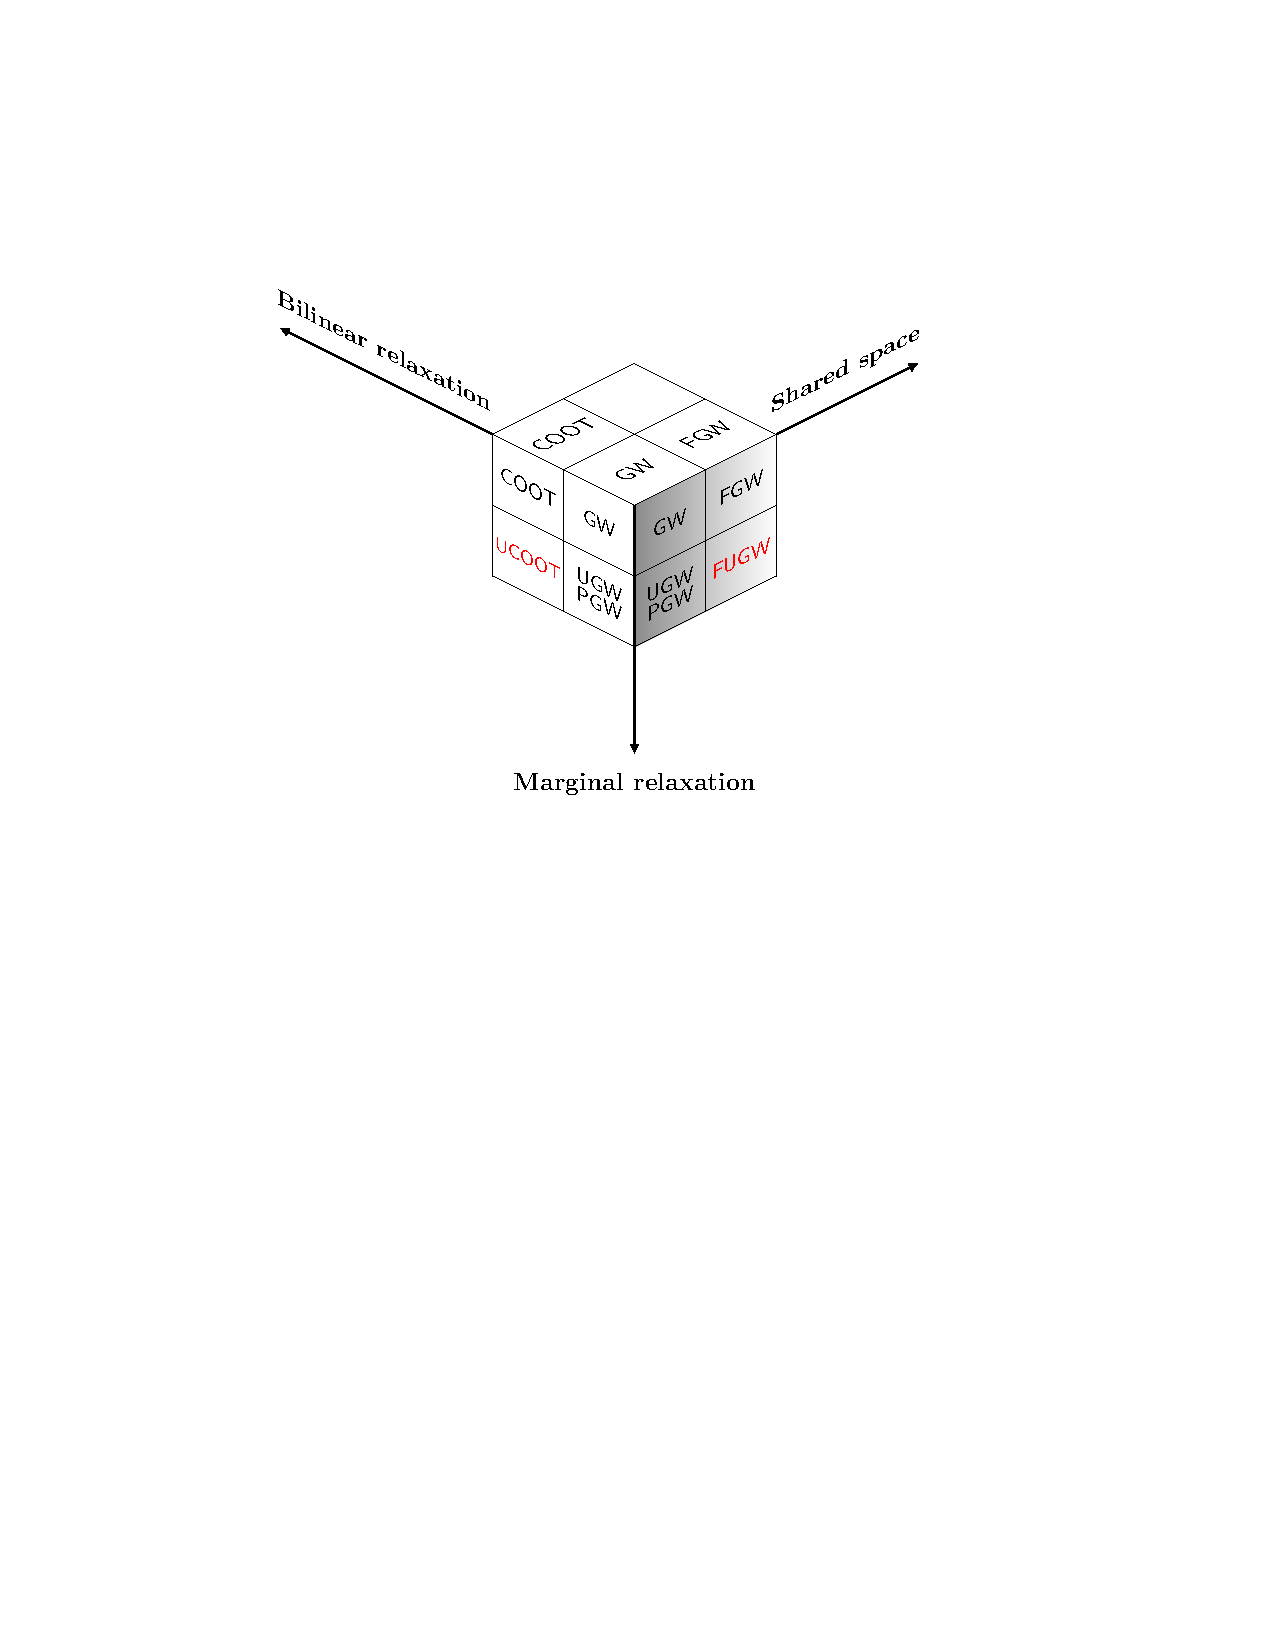
\includegraphics[scale=0.35]{OT_new/cube_fugw.pdf}};
\end{tikzpicture}

\end{frame}

%%%%%%%%%%%%%%%%%%%%%%%%%%%%%
\begin{frame}{Experimental results (with Alexis Thual)}
% \vspace{-0.5cm}
\scriptsize
\begin{itemize}
  \item[$\bullet$] Learn transport plan from train functional maps, predict on test functional maps.
  \item[$\bullet$] Evaluation metric = $\text{corr}(\text{transported features}, \text{target features})$.
  \item[$\bullet$] Baseline = $\text{corr}(\text{proj}_{\text{source features}}, \text{proj}_{\text{target features}})$.
\end{itemize}
\begin{figure}
  \centering
  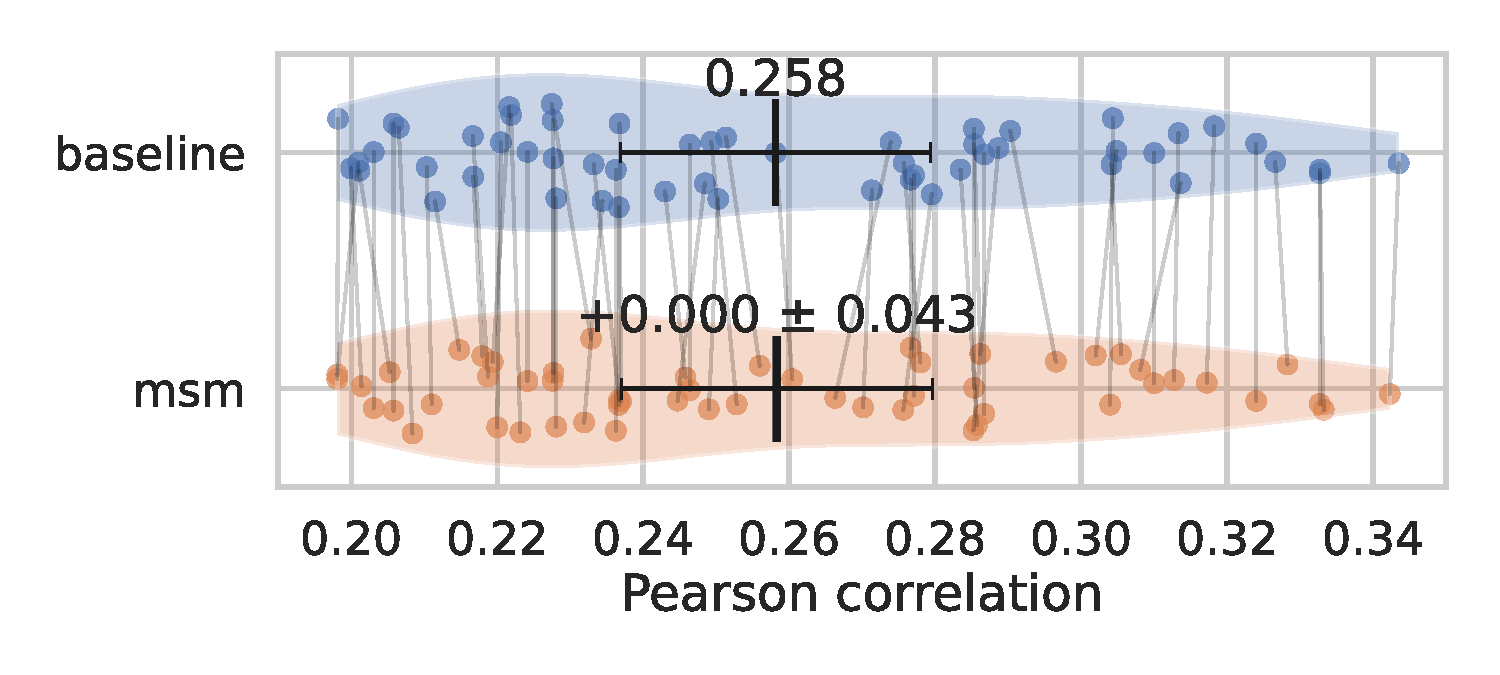
\includegraphics[width=0.49\linewidth, keepaspectratio=true]{OT_new/fsaverage5_alignment_correlation_gain_msm.pdf}
  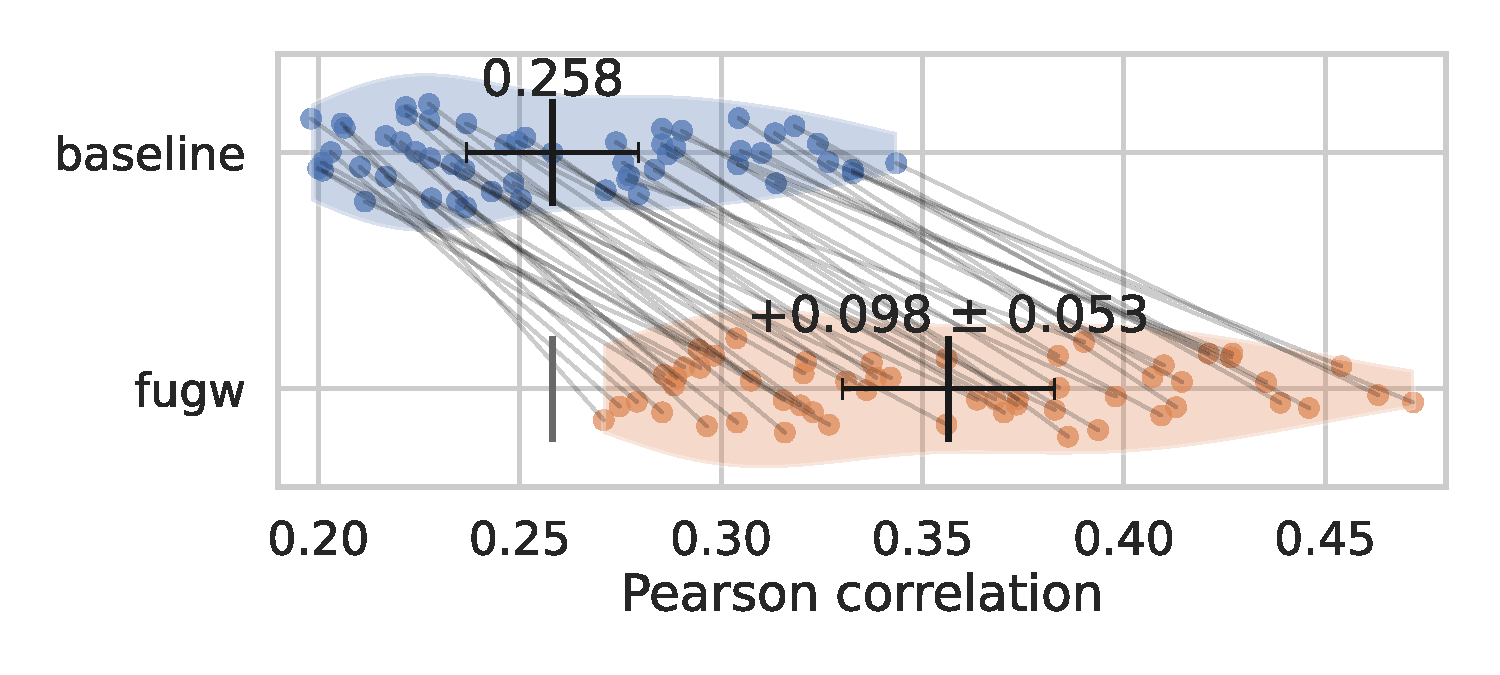
\includegraphics[width=0.49\linewidth, keepaspectratio=true]{OT_new/fsaverage5_alignment_correlation_gain_fugw.pdf}
  \caption*{\scriptsize{Comparison of gains in correlation after inter-subject alignment.}}
\end{figure}

\vspace{-0.2cm}
\begin{figure}
  \centering
  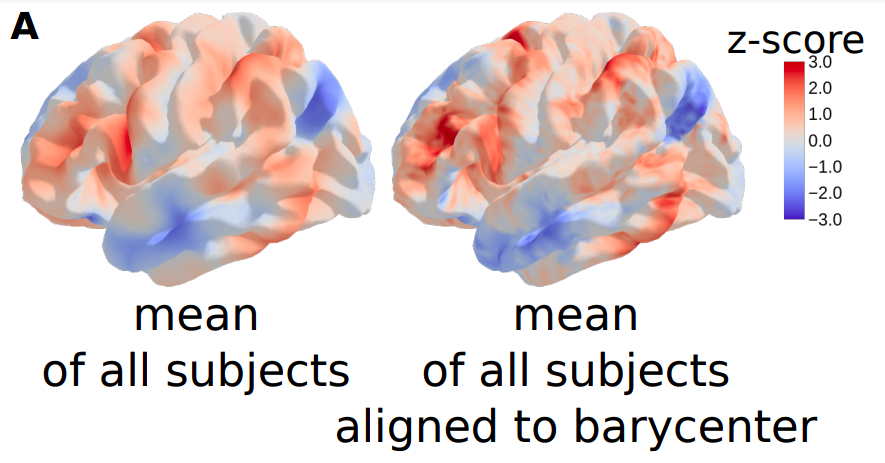
\includegraphics[width=0.4\linewidth, keepaspectratio=true]{OT_new/brain_template.png}
  \caption*{\scriptsize{FUGW barycenter vs group average.}}
\end{figure}

\begin{tikzpicture}[remember picture, overlay]
  \node[shift={(-3.7cm,-6.3cm)}] at (current page.center)
  {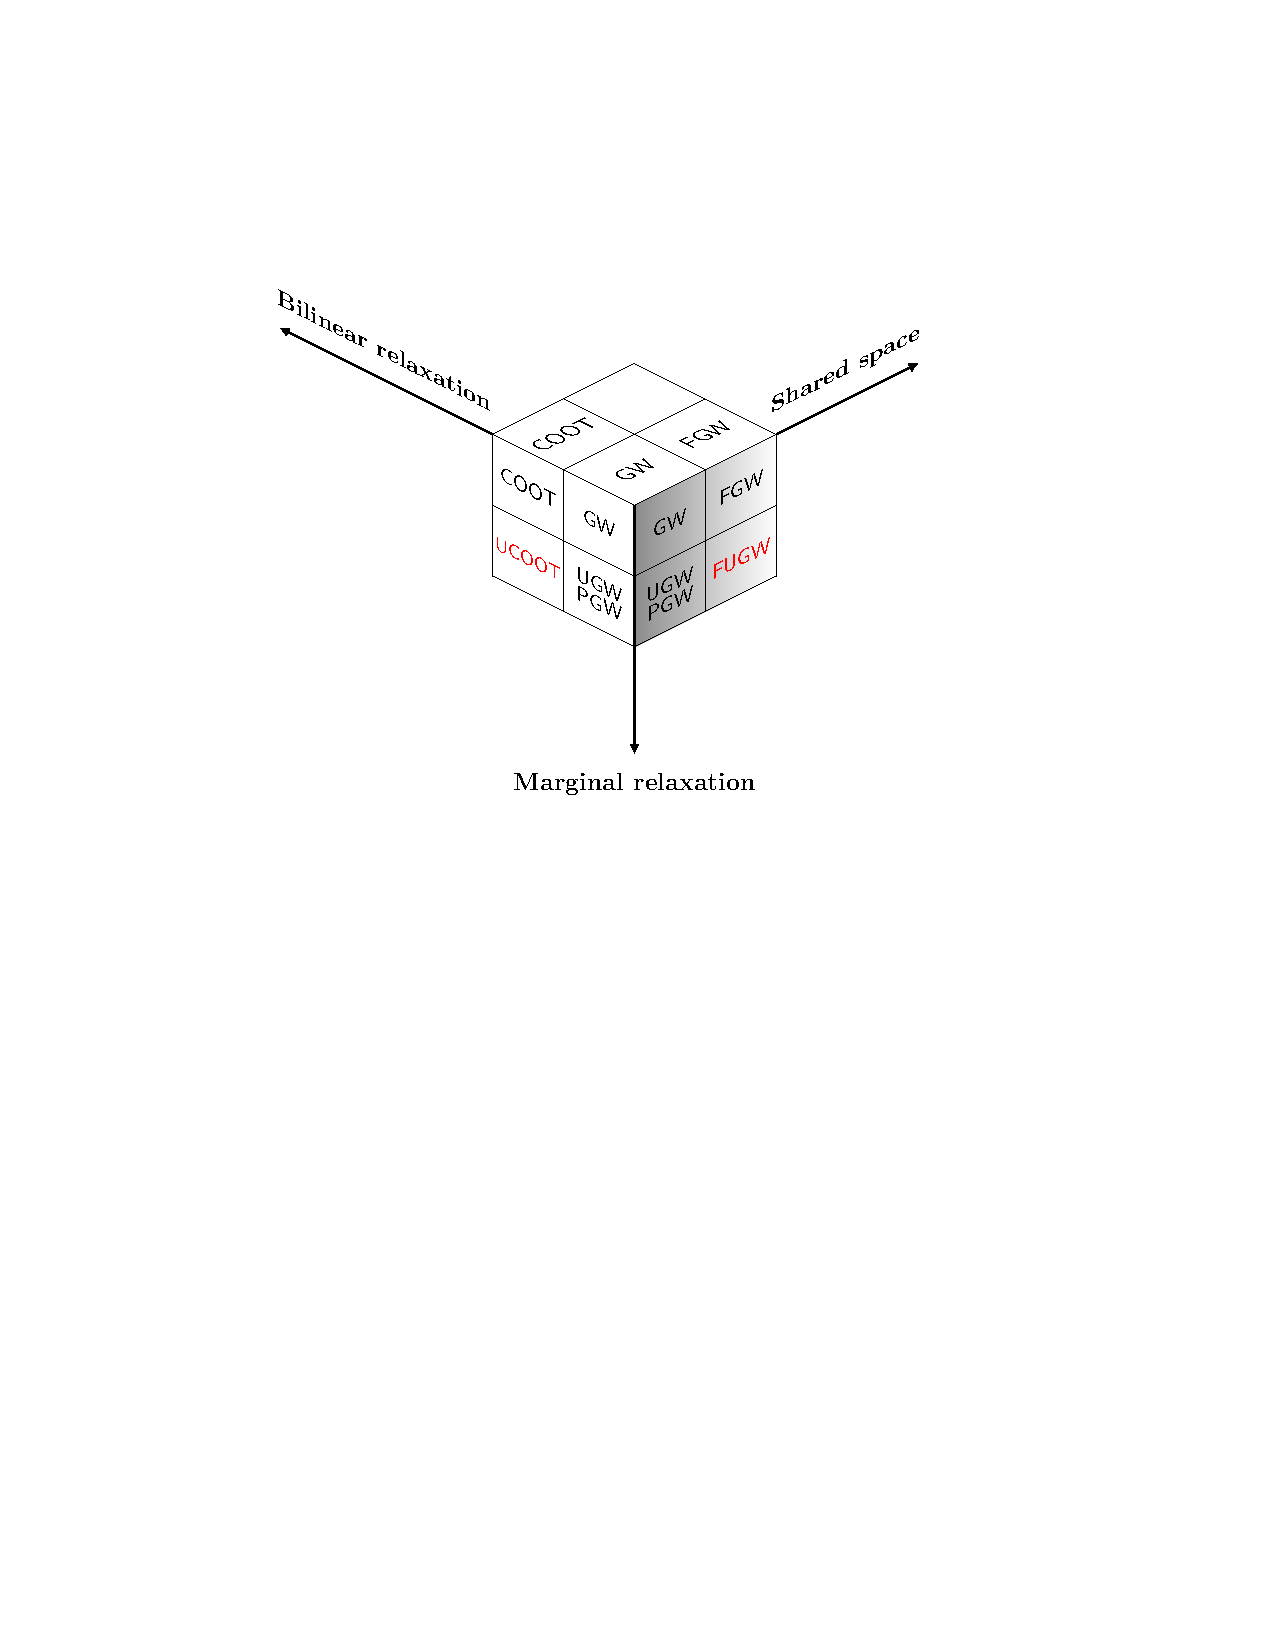
\includegraphics[scale=0.35]{OT_new/cube_fugw.pdf}};
\end{tikzpicture}

\end{frame}

%%%%%%%%%%%%%%%%%%%%%%%%%%%%%%%%%%%%%%%%%%%%%%%%%%%%%%%%%%%%%%%%%%%%%%
%%%%%%%%%%%%%%%%%%%%%%%%%%%%%%%%%%%%%%%%%%%%%%%%%%%%%%%%%%%%%%%%%%%%%%
%%%%%%%%%%%%%%%%%%%%%%%%%%%%%%%%%%%%%%%%%%%%%%%%%%%%%%%%%%%%%%%%%%%%%%
%%%% Contribution on UCOOT
\section{Unbalanced CO-Optimal Transport}

%%%%%%%%%%%%%%%%%%%%%%%%%%%%%%%%%%%%
\begin{frame}{Alignment with CO-Optimal Transport}
  \scriptsize
  \vspace*{0.5cm}
  \begin{itemize}
    \setlength\itemsep{0.2cm}
    \item[$\bullet$] $X \in \bbR^{{\color{blue}{20}} \times {\color{red}{16}}}: X_{ij} = \cos({\color{blue}{\frac{i}{20}}} \pi) + \cos({\color{red}{\frac{j}{16}}} \pi)$.
    \item[$\bullet$] $Y \in \bbR^{{\color{blue}{10}} \times {\color{red}{8}}}: Y_{ij} = \cos({\color{blue}{\frac{i}{10}}} \pi) + \cos({\color{red}{\frac{j}{8}}} \pi)$.
  \end{itemize}
  \vspace*{-0.2cm}
  \begin{figure}
    \centering
    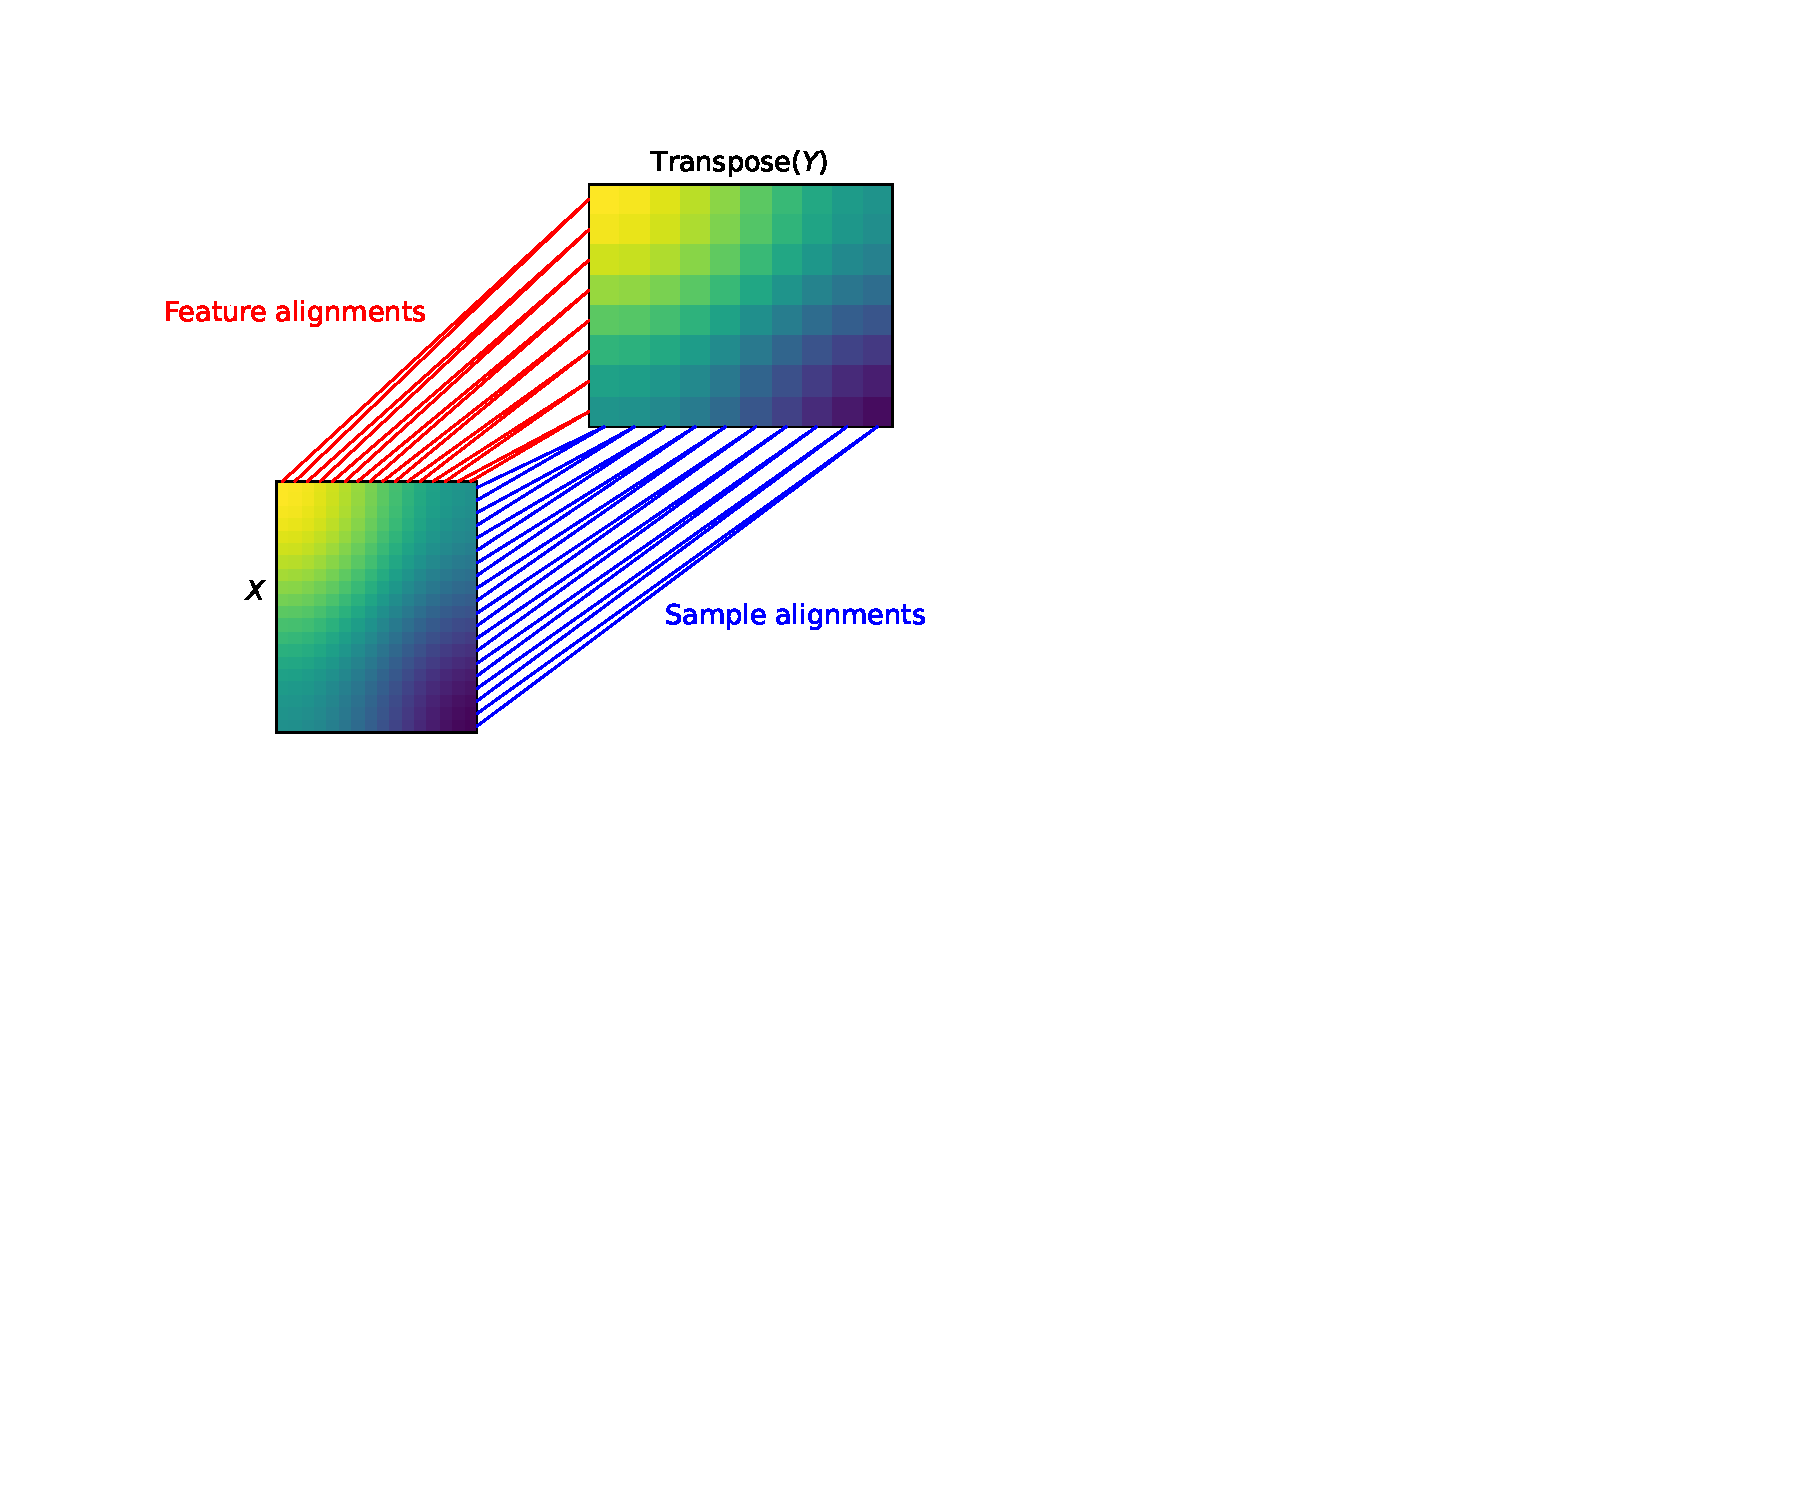
\includegraphics[width=1.4\linewidth, keepaspectratio=true]{OT_new/UCOOT_plot_intro.pdf}
  \end{figure}
\end{frame}

%%%%%%%%%%%%%%%%%%%%%%%%%%%%%%%%%%%%
\begin{frame}{Motivation: alignments under presence of outliers (1)}
\scriptsize
\begin{figure}
  \centering
  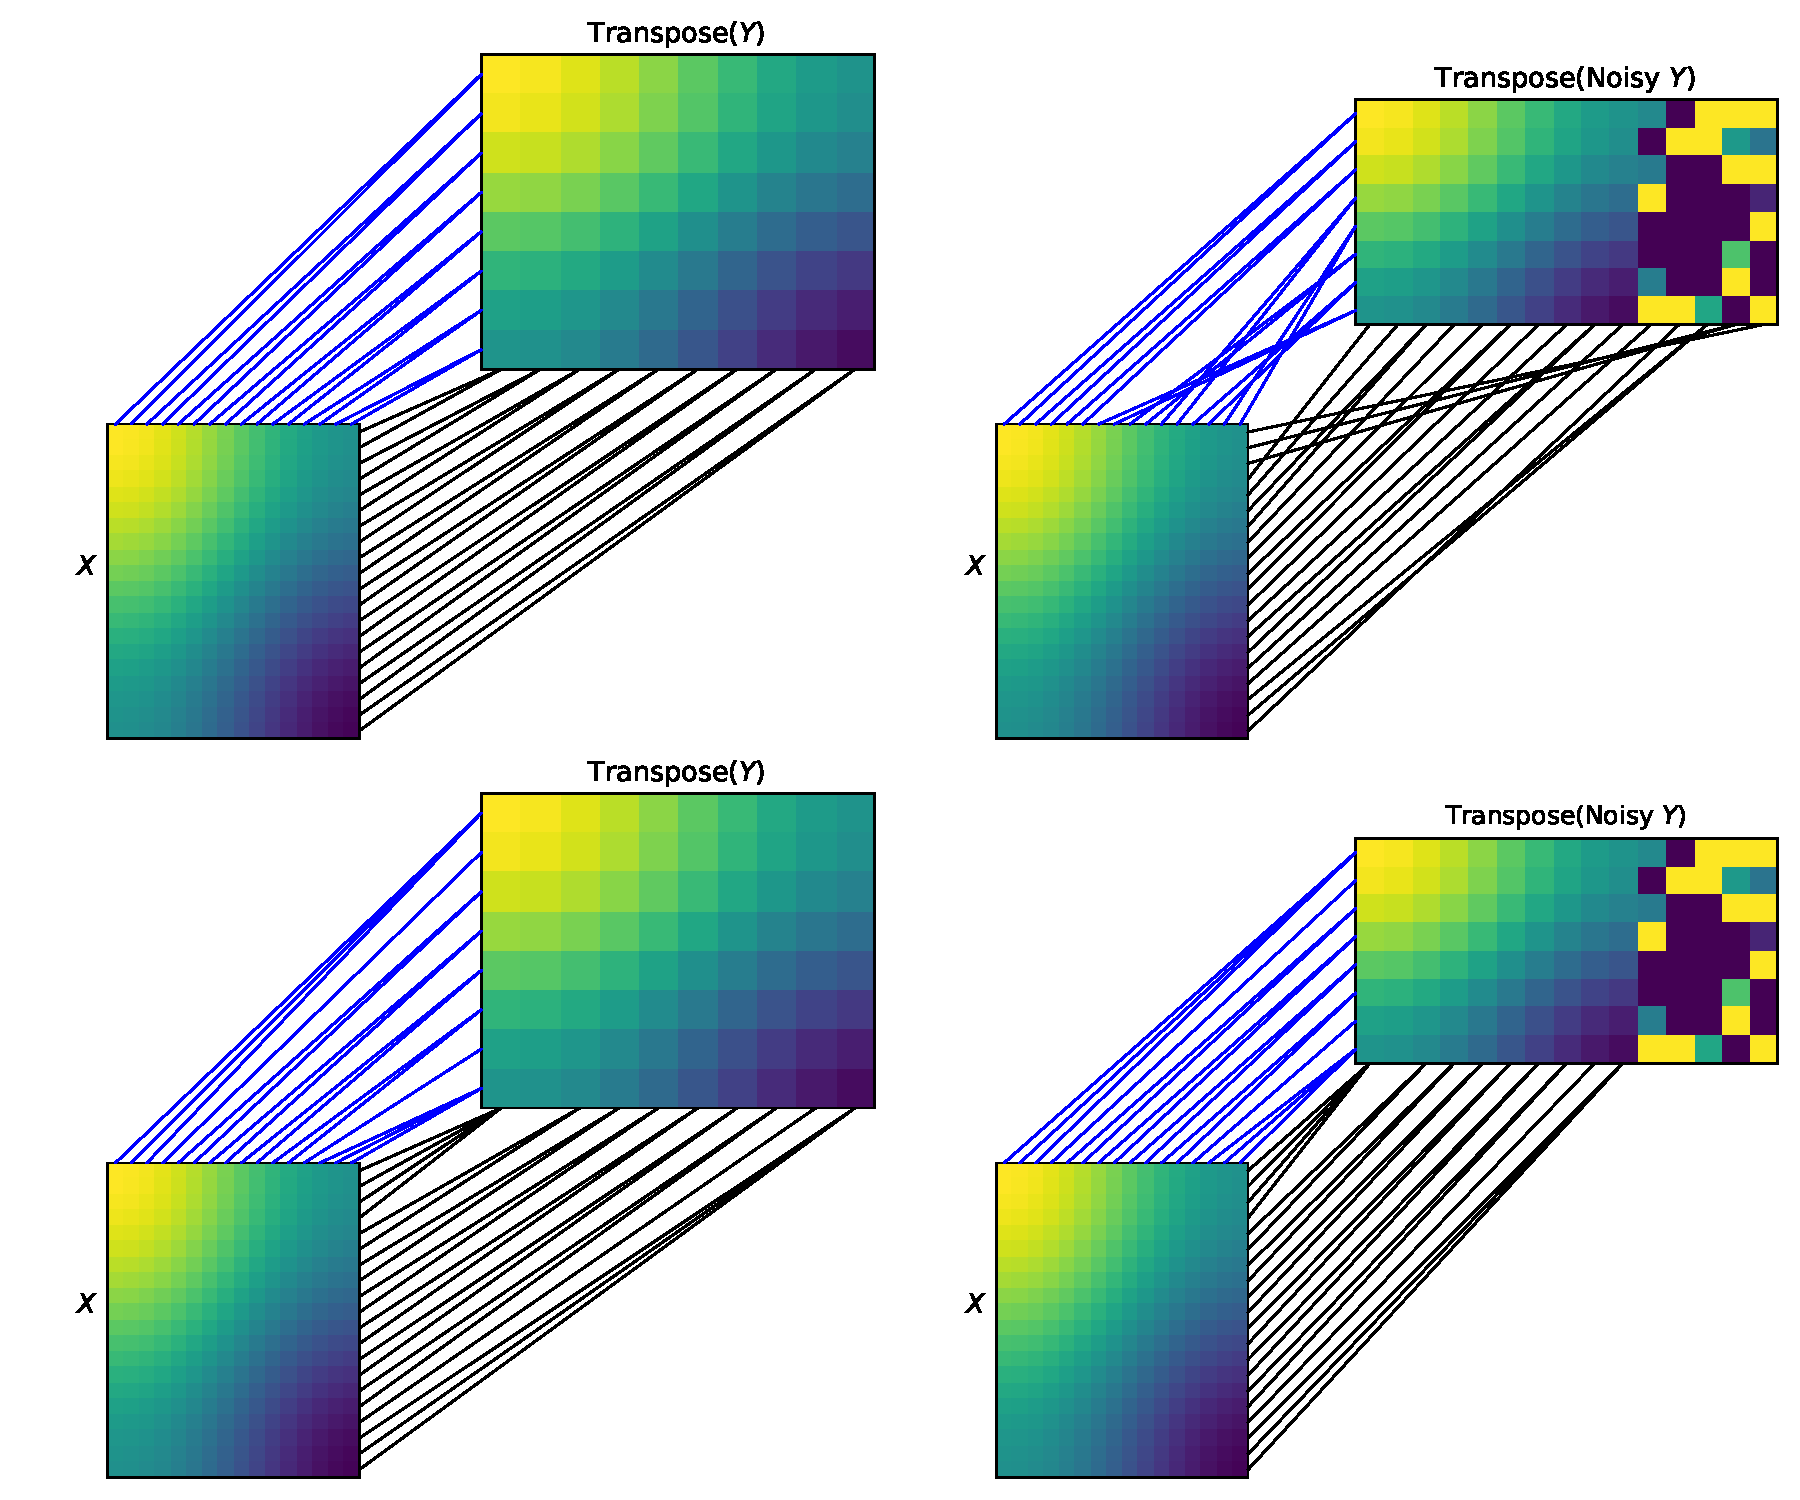
\includegraphics[width=0.9\linewidth, keepaspectratio=true]{OT_new/COOT_plot.pdf}
\end{figure}
\begin{tikzpicture}[remember picture, overlay]
  % we don't want to affect the bounding box if the rectangle is too large
  \begin{pgfinterruptboundingbox}
      % the following coords. may need to be changed to suit your slides
      \fill <1> [fill=white, opacity=0.8] (0,0) rectangle (12, 4.5);
  \end{pgfinterruptboundingbox}
  \node <1> [draw, shape=rectangle, align=right] at (10, 5.3) {%
      Hello from outliers
  };
\end{tikzpicture}
\end{frame}

%%%%%%%%%%%%%%%%%%%%%%%%%%%%%%%%%%%%
\begin{frame}{Motivation: alignments under presence of outliers (2)}
  \scriptsize
  \begin{figure}
    \centering
    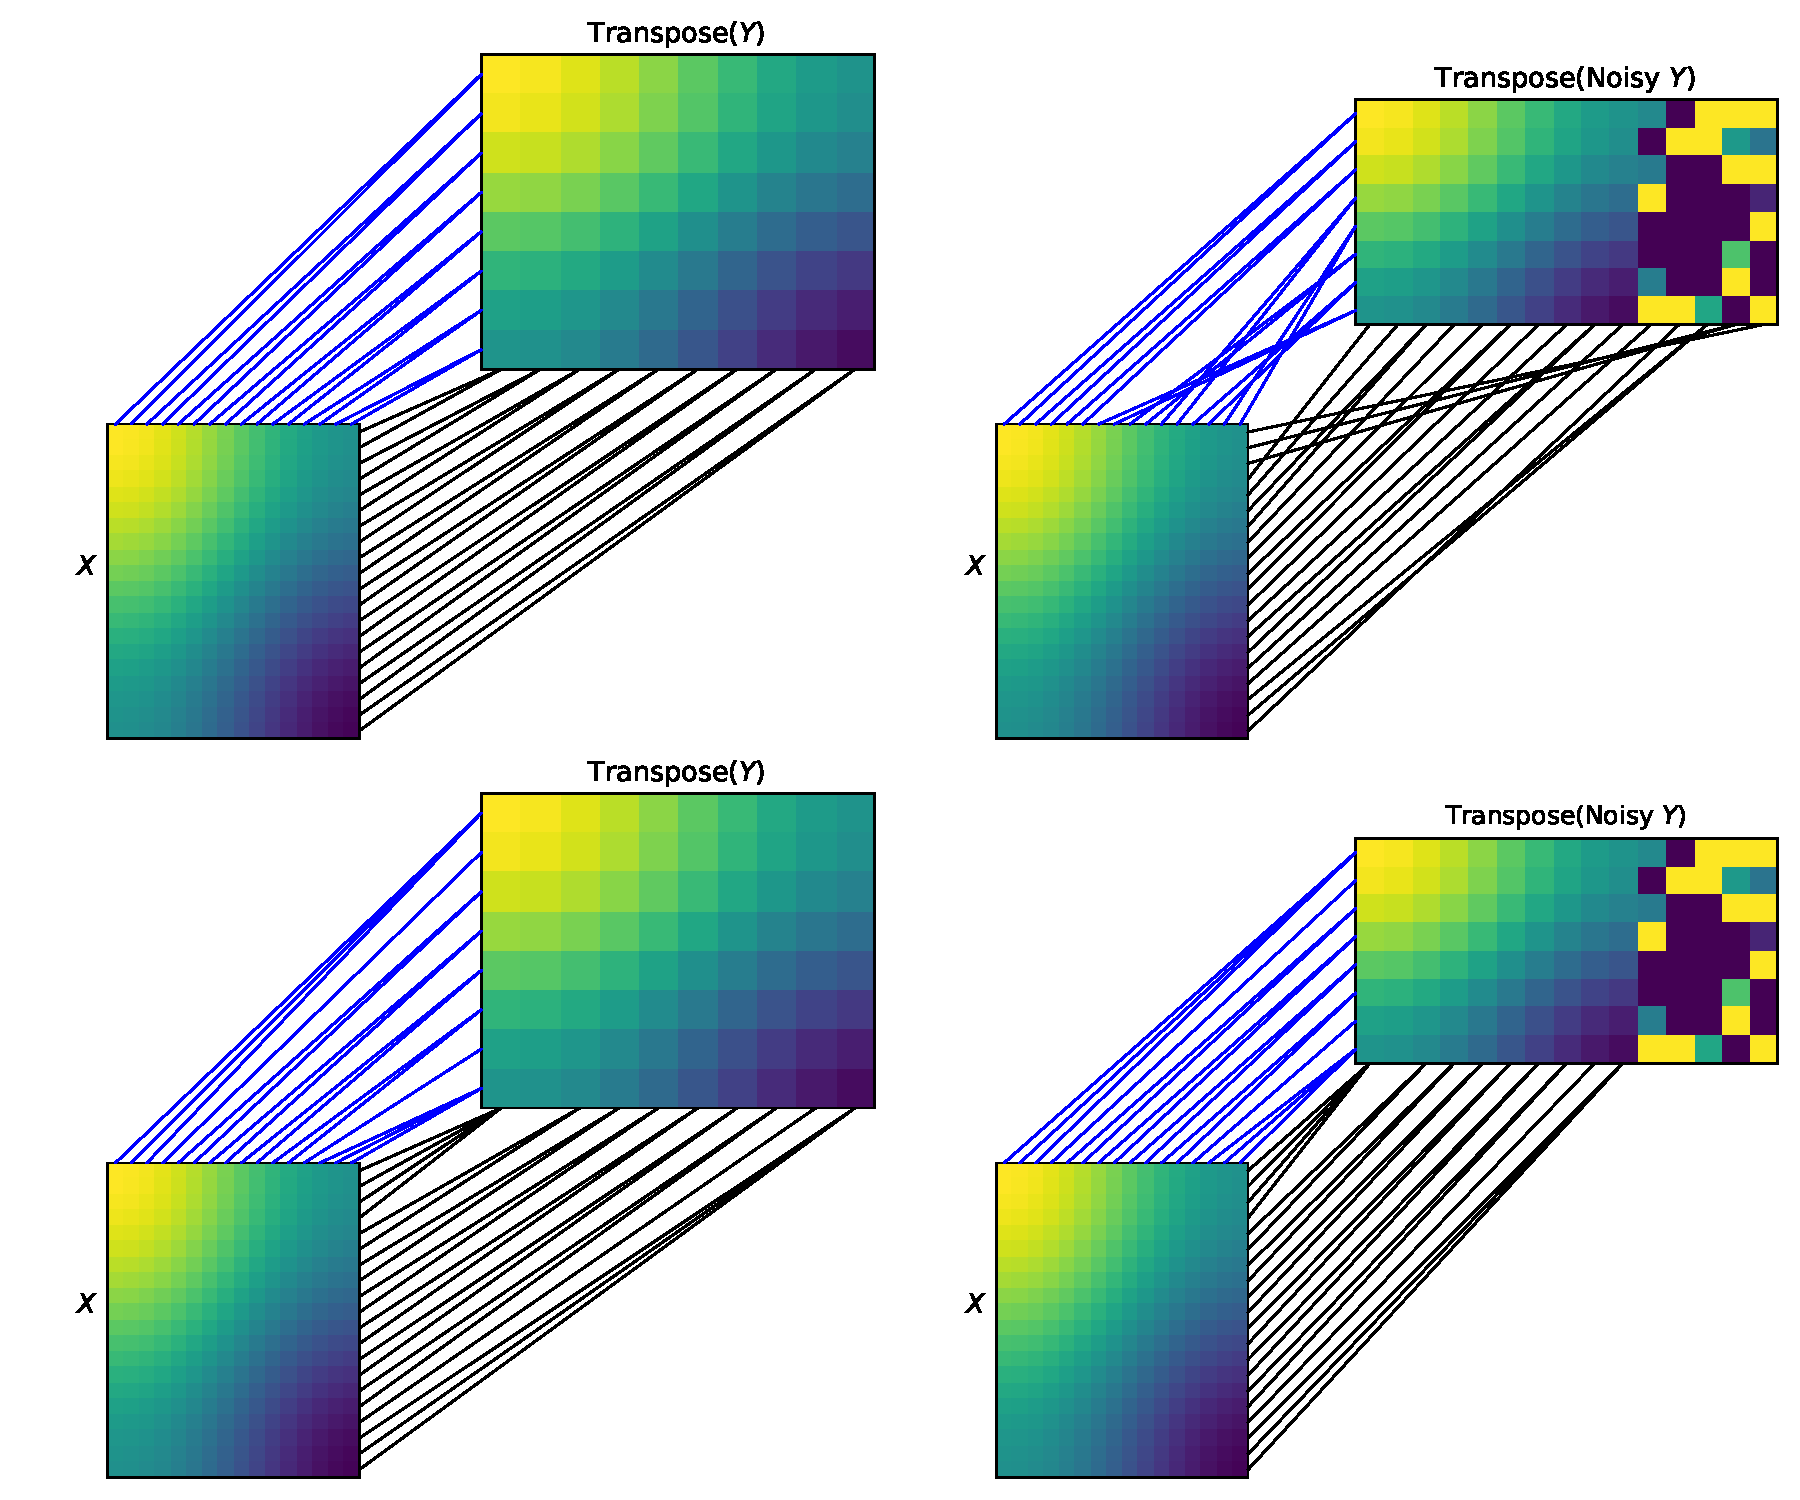
\includegraphics[width=0.9\linewidth, keepaspectratio=true]{OT_new/COOT_plot.pdf}
  \end{figure}
  \begin{tikzpicture}[remember picture, overlay]
    % we don't want to affect the bounding box if the rectangle is too large
    \begin{pgfinterruptboundingbox}
        % the following coords. may need to be changed to suit your slides
        \fill <1> [fill=white, opacity=0.8] (0,4.57) rectangle (12, 8.7);
    \end{pgfinterruptboundingbox}
    \node <1> [draw, shape=rectangle, align=right] at (10.2, 1.6) {%
        Goodbye outliers
    };
  \end{tikzpicture}
\end{frame}

%%%%%%%%%%%%%%%%%%%%%%%%%%%%%%%%%%%%%%%%%%%
\begin{frame}{Unbalanced Co-Optimal Transport}
  \scriptsize

  \begin{tikzpicture}[remember picture, overlay]
    \node[shift={(0cm,-1.5cm)}] at (current page.center)
    {\includegraphics[scale=0.55]{OT_new/cube_ucoot_contrib.pdf}};
  \end{tikzpicture}

  \vspace{5cm}
  {\color{brown}{\textbf{Summary}}}:
  \begin{enumerate}
    \setlength\itemindent{10pt}
    \item[1.] Unbalanced formulation of COOT which is provably robust to outliers.
    \item[2.] Applications to heterogeneous domain adaptation and single-cell multi-omics.
  \end{enumerate}

  \vspace{0.3cm}
  {\color{brown}{\textbf{Publication}}}: Unbalanced Co-Optimal Transport.
  QHT, Hicham Janati, Nicolas Courty, Rémi Flamary, Ievgen Redko,
  Pinar Demetci, and Ritambhara Singh.
  AAAI Conference on Artificial Intelligence, 2023.

\end{frame}

%%%%%%%%%%%%%%%%%%%%%%%%%%%%%%%%%%%%
\begin{frame}{Formulation (1)}
\scriptsize
  \begin{definition}[{\color{blue}{Sample}} - {\color{red}{feature}} space]
    Let ${\color{blue}{(X^s, \mu^s)}}$ and ${\color{red}{(X^f, \mu^f)}}$ be compact measure spaces, where ${\color{blue}{\mu^s \in \cM^+(X^s)}}$ and ${\color{red}{\mu^f \in \cM^+(X^f)}}$. Let $c$ be a scalar integrable function in $L^p({\color{blue}{X^s}} \times {\color{red}{X^f}}, {\color{blue}{\mu^s}} \otimes {\color{red}{\mu^f}})$, for some $p \geq 1$. We call
    \begin{itemize}
      \setlength\itemindent{10pt}
      \item[$\bullet$] The triplet
      $\cX = \left({\color{blue}{(X^s, \mu^s)}}, {\color{red}{(X^f, \mu^f)}}, c \right)$
      a \underline{\textit{{\color{blue}{sample}} - {\color{red}{feature}} space}}
      (\sfspace space).

      \item[$\bullet$] The function $c$ an \textit{\underline{interaction}}.
    \end{itemize}
  \end{definition}
  \begin{itemize}
    \setlength\itemindent{5pt}
    \item[$\bullet$] Ours $\neq$ \parencite{Chowdhury21b}: bounded measurable function on measure spaces.
  \end{itemize}

  \begin{tikzpicture}[remember picture, overlay]
    \node[shift={(-3.7cm,-6.3cm)}] at (current page.center)
    {\includegraphics[scale=0.35]{OT_new/cube_ucoot.pdf}};
  \end{tikzpicture}

  \vspace{-0.3cm}
  \begin{minipage}[t]{0.6\linewidth}
  \end{minipage}%
  \hfill%
  \begin{minipage}[t]{0.8\linewidth}
  \begin{figure}
    \centering
    \includegraphics[width=\linewidth, keepaspectratio=true]{OT_new/coot_matrix_single.pdf}
  \end{figure}
  \end{minipage}

\end{frame}

%%%%%%%%%%%%%%%%%%%%%%%%%%%%%%%%%%%%%%%%%%%%%%%%%%%
\begin{frame}{Formulation (2)}
\scriptsize
\vspace{-0.8cm}
\begin{definition}[UCOOT]
  Given $\lambda_1, \lambda_2 >0$, the unbalanced COOT of order $p \geq 1$
  between two \sfspace spaces $\cX_1 = \left({\color{blue}{(X_1^s, \mu_1^s)}}, {\color{red}{(X_1^f, \mu_1^f)}}, c_1 \right)$
  and $\cX_2 = \left({\color{blue}{(X_2^s, \mu_2^s)}}, {\color{red}{(X_2^f, \mu_2^f)}}, c_2 \right)$ is defined by
  \begin{align*}
\label{eq:ucoot}
    \ucoot_{\lambda}(\cX_1, \cX_2) :=
  \inf_{\substack{{\color{blue}{\pi^s \in \cM^+(X_1^s \times X_2^s)}}
  \\ {\color{red}{\pi^f \in \cM^+(X_1^f \times X_2^f)}}}}
  \cL_{\ucoot}(\pis, \pif).
\end{align*}
\vspace{-0.8cm}
where:
\begin{align*}
    \cL_{\ucoot}(\pis, \pif) &= \underbrace{\iint
    |c_1({\color{blue}{x_1^s}}, {\color{red}{x_1^f}}) - c_2({\color{blue}{x_2^s}}, {\color{red}{x_2^f}})|^p \; {\color{blue}{\mathrm d\pi^s(x_1^s, x_2^s)}} \;
    {\color{red}{\mathrm d \pi^f(x_1^f, x_2^f)}}}_{\text{transport cost of {\color{blue}{sample}}-{\color{red}{feature}} pairs}} \\
    &+ \underbrace{\sum_{k=1}^2\lambda_k \; \text{KL}({\color{blue}{\pi^s_{\# k}}} \otimes {\color{red}{\pi^f_{\# k}}} \vert {\color{blue}{\mu^s_k}} \otimes {\color{red}{\mu^f_k}})}_{\text{mass destruction / creation penalty}}.
\end{align*}
\end{definition}

\begin{itemize}
  \item[$\bullet$] If ${\color{blue}{\mu^s_k}} = {\color{red}{\mu^f_k}}$ $\Rightarrow$
  Encoding same (weak) isomorphisms as COOT.
  \item[$\bullet$] Quadratic divergence $\Rightarrow$ Provable robustness.
\end{itemize}
% {\color{brown}{\textbf{Why quadratic divergence?}}}
% \begin{itemize}
%   \item[$\bullet$] UCOOT = UOT under additional factorization constraint
%   $\Rightarrow$ Existence of solution.

%   \item[$\bullet$] Restriction to equal-mass solutions: $m({\color{blue}{\pi^s_*}}) = m({\color{red}{\pi^f_*}})$.

%   $\Rightarrow$ Numerical stability when solving with entropic regularization.

%   \item[$\bullet$] Provable robustness to outliers.
% \end{itemize}

\begin{tikzpicture}[remember picture, overlay]
  \node[shift={(-3.7cm,-6.3cm)}] at (current page.center)
  {\includegraphics[scale=0.35]{OT_new/cube_ucoot.pdf}};
\end{tikzpicture}

\end{frame}

%%%%%%%%%%%%%%%%%%%%%%%%%
\begin{frame}{Robustness property (1)}
\scriptsize
  \begin{definition}[Noisy {\color{blue}{sample}} - {\color{red}{feature}} space]
  Given two \textbf{clean} \sfspace spaces
  $\cX_1 = \left({\color{blue}{(X_1^s, \mu_1^s)}}, {\color{red}{(X_1^f, \mu_1^f)}}, c_1 \right),
  \cX_2 = \left({\color{blue}{(X_2^s, \mu_2^s)}}, {\color{red}{(X_2^f, \mu_2^f)}}, c_2 \right)$.
  \begin{enumerate}
    \setlength\itemindent{5pt}
    \item[1.] \textbf{Noisy} \sfspace space: $\widetilde{\cX_1} = \left( {\color{blue}{(X^s_1 \cup O^s, \widetilde{\mu}^s_1)}}, {\color{red}{(X^f_1 \cup O^f, \widetilde{\mu}^f_1)}}, c_1 \right)$, where
    \begin{itemize}
      \scriptsize
      \setlength\itemindent{10pt}
        \item[$\bullet$] {\color{blue}{\textbf{Noisy} sample measure:
        $\widetilde{\mu}^s_1 = \alpha_s \mu^s_1 + (1-\alpha_s) \varepsilon^s$, for $\alpha_s \in [0,1], \varepsilon^s \in \cM^+(O^s)$.}}
        \item[$\bullet$] {\color{red}{\textbf{Noisy} feature measure:
        $\widetilde{\mu}^f_1 = \alpha_f \mu^f_1 + (1-\alpha_f) \varepsilon^f$, for $\alpha_f \in [0,1], \varepsilon^f \in \cM^+(O^f)$.}}
    \end{itemize}

    \item[2.] Minimal cost: $\Delta_{0} := \min_{\substack{
      {\color{blue}{x_1^s \in O^s}}, {\color{red}{x_1^f \in O^f}} \\
      {\color{blue}{x_2^s \in X_2^s}}, {\color{red}{x_2^f \in X_2^f}}}}\quad \left| c_1({\color{blue}{x_1^s}}, {\color{red}{x_1^f}}) - c_2({\color{blue}{x_2^s}}, {\color{red}{x_2^f}}) \right|^p$.

    \item[3.] Maximal cost: $\Delta_{\infty} := \max_{
    \substack{
    {\color{blue}{x_1^s \in X_1^s \cup O^s}}, {\color{red}{x_1^f \in X_1^f \cup O^f}} \\
    {\color{blue}{x_2^s \in X_2^s}}, {\color{red}{x_2^f \in X_2^f}}
    }} \quad \left| c_1({\color{blue}{x_1^s}}, {\color{red}{x_1^f}}) - c_2({\color{blue}{x_2^s}}, {\color{red}{x_2^f}}) \right|^p$.
  \end{enumerate}
  \end{definition}

  \begin{minipage}[t]{0.7\linewidth}
    $\Rightarrow$ Both costs can explode if the outliers are too impactful.
  \end{minipage}%
    \hfill%
    \hspace{-6cm}
    \begin{minipage}[t]{0.35\linewidth}
      \vspace{-0.5cm}
    \begin{figure}
      \centering
      \includegraphics[width=1.1\linewidth, keepaspectratio=true]{OT_new/noisy_toy.pdf}
    \end{figure}
  \end{minipage}

  \begin{tikzpicture}[remember picture, overlay]
    \node[shift={(-3.7cm,-6.3cm)}] at (current page.center)
    {\includegraphics[scale=0.35]{OT_new/cube_ucoot.pdf}};
  \end{tikzpicture}

\end{frame}

\begin{frame}{Robustness property (2)}
\scriptsize
\vspace{-0.2cm}
\begin{proposition}
  \begin{enumerate}
    % \setlength\itemsep{0em}
    \setlength\itemindent{5pt}
    \item[1.] COOT is sensitive to outliers:
    $\coot(\widetilde{\cX_1}, \cX_2) \geq (1 - {\color{blue}{\alpha_s}})(1 - {\color{red}{\alpha_f}})\Delta_0$.

    \item[2.] UCOOT is robust to outliers: denote
    \begin{itemize}
      \scriptsize
      \setlength\itemindent{10pt}
      \item[$\bullet$] $\delta = 2(\lambda_1 + \lambda_2)(1 - {\color{blue}{\alpha_s}} {\color{red}{\alpha_f}})$.

      \item[$\bullet$] $M= m(\pis) = m(\pif)$: mass of OT plans between clean data.

      \item[$\bullet$] $K = M + \frac{1}{M}\ucoot_{\lambda}(\cX_1, \cX_2) + \delta$.
    \end{itemize}
    Then,
    \vspace{-0.4cm}
    \begin{equation*} %\label{eq:ucoot-robust}
    \begin{split}
      \underbrace{\ucoot_{\lambda}(\widetilde{\cX_1}, \cX_2)}_{\text{"noisy divergence"}}
      &\leq {\color{blue}{\alpha_s}} {\color{red}{\alpha_f}}
      \underbrace{\ucoot_{\lambda}(\cX_1, \cX_2)}_{\text{"clean divergence"}}
      + \underbrace{\delta M \left[ 1 -
      \exp \left( {- \frac{\Delta_{\infty}(1+M) + K}{\delta M}} \right) \right]}_{\text{saturates quickly if } \Delta_{\infty} \to \infty}.
    \end{split}
    \end{equation*}
  \end{enumerate}

  \begin{tikzpicture}[remember picture, overlay]
    \node[shift={(-3.7cm,-6.3cm)}] at (current page.center)
    {\includegraphics[scale=0.35]{OT_new/cube_ucoot.pdf}};
  \end{tikzpicture}
\end{proposition}

\begin{minipage}[t]{0.6\linewidth}
  \begin{itemize}
    \item[$\bullet$] UCOOT is always upper bounded.
    \item[$\bullet$] Robustness also holds for unbalanced GW.
  \end{itemize}
\end{minipage}%
\hfill%
\hspace{-6cm}
\begin{minipage}[t]{0.47\linewidth}
  \vspace{-0.3cm}
  \begin{figure}
    \centering
    \includegraphics[width=1.05\linewidth, keepaspectratio=true]{SIMPAS/robustness_2.pdf}
  \end{figure}
\end{minipage}

\begin{tikzpicture}[remember picture, overlay]
  \node[shift={(-3.7cm,-6.3cm)}] at (current page.center)
  {\includegraphics[scale=0.35]{OT_new/cube_ucoot.pdf}};
\end{tikzpicture}

\end{frame}

%%%%%%%%%%%%%%%%%%%%%%%%%%%%%%%%%
\begin{frame}{Illustration 1: MNIST images}
\scriptsize
\begin{itemize}
  \item[$\bullet$] Feature outliers = Gaussian noise of shape $28 \times 6$.
  \item[$\bullet$] Sample outliers = Gaussian noise of shape $28 \times 34$.
\end{itemize}
\vspace{-0.5cm}
\begin{figure}
    \centering
    \includegraphics[width=1.05\linewidth, keepaspectratio=true]{SIMPAS/mnist-ucoot-rebuttal.pdf}
    \vspace*{-1cm}
    % \caption*{\scriptsize{Example illustrating and interpreting
    % the {\color{red}{feature alignment $\pi^f$}} learned by UCOOT
    % and its robustness to outliers.}}
\end{figure}

\begin{tikzpicture}[remember picture, overlay]
  \node[shift={(-3.7cm,-6.3cm)}] at (current page.center)
  {\includegraphics[scale=0.35]{OT_new/cube_ucoot.pdf}};
\end{tikzpicture}

\end{frame}

%%%%%%%%%%%%%%%%%%%%%%%%%%%%%%%%%
\begin{frame}{Illustration 2: Single-cell multi-omics (with Pinar Demetci)}
\scriptsize
\vspace{-0.2cm}
\begin{itemize}
  \item[$\bullet$] Dataset: CITE-Seq \parencite{CITEseq}
  \begin{itemize}
    \scriptsize
    \setlength\itemindent{10pt}
    \item[$+$] Source: sample = cells, features = antibodies.
    \item[$+$] Target: samples = same cells, features = gene expressions.
  \end{itemize}
\end{itemize}
\vspace{-0.5cm}
\begin{figure}
      \centering
      \includegraphics[width=1.05\linewidth, keepaspectratio=true]{OT_new/genes-alignments.pdf}
      % \caption*{\scriptsize{Example illustrating and interpreting the
      % {\color{red}{feature alignment $\pi^f$}} learned by UCOOT
      % and its robustness to outliers.}}
  \end{figure}

  \begin{tikzpicture}[remember picture, overlay]
    \node[shift={(-3.7cm,-6.3cm)}] at (current page.center)
    {\includegraphics[scale=0.35]{OT_new/cube_ucoot.pdf}};
  \end{tikzpicture}
\end{frame}

%%%%%%%%%%%%%%%%%%%%%%%%%%%%%%%%%%%%%%%%%%%%%%%%%%%%%%%%%%%%%%%%%%%%%%
%%%%%%%%%%%%%%%%%%%%%%%%%%%%%%%%%%%%%%%%%%%%%%%%%%%%%%%%%%%%%%%%%%%%%%
%%%%%%%%%%%%%%%%%%%%%%%%%%%%%%%%%%%%%%%%%%%%%%%%%%%%%%%%%%%%%%%%%%%%%%
%%%% Contribution on AGW
\section{Augmented Gromov-Wasserstein}

%%%%%%%%%%%%%%%%%%%%%%%%%%%%%%%%%%%%%%
\begin{frame}{Isometries: too flexible vs too rigid}
%%%%%%%%%%%%%%%%%%%%%%%%%%%%%%%%%
\scriptsize

\begin{enumerate}
  \item[1.] Isometries are useful for across-space comparison.
  \item[2.] Isometry farm: all isometries are created equal, but some are more equal than others.
  \item[3.] GW induces all isometries but maybe too many.
  \item[4.] COOT is good at exploiting data but maybe too rigid with isometries.
\end{enumerate}
\begin{figure}
    \centering
    \includegraphics[width=1.05\linewidth, keepaspectratio=true]{OT_new/div_vs_angle.pdf}
\end{figure}

\end{frame}

%%%%%%%%%%%%%%%%%%%%%%%%%%%%%%%%%%%%%%%%%%
\begin{frame}{Augmented Gromov-Wasserstein}
  \scriptsize

  \begin{tikzpicture}[remember picture, overlay]
    \node[shift={(0cm,-1.5cm)}] at (current page.center)
    {\includegraphics[scale=0.55]{OT_new/cube_agw_contrib.pdf}};
  \end{tikzpicture}

  \vspace{5cm}
  {\color{brown}{\textbf{Summary}}}:
  \begin{enumerate}
    \setlength\itemindent{10pt}
    \item[1.] Interpolation between GW and COOT to get the best from both worlds.
    \item[2.] Applications to heterogeneous domain adaptation and single-cell multi-omics.
  \end{enumerate}

  \vspace{0.3cm}
  {\color{brown}{\textbf{Publication}}}: Breaking isometric ties and introducing priors in Gromov-Wasserstein distances.
  Pinar Demetci, QHT, Ievgen Redko, and Ritambhara Singh.
  International Conference on Artificial Intelligence and Statistics (AISTATS), 2024.

\end{frame}

%%%%%%%%%%%%%%%%%%%%%%%%%%%%%%%%%%%%%%
\begin{frame}{Formulation}
\scriptsize
\begin{block}{Definition}
  For $0\leq \alpha \leq 1$, the Augmented GW divergence between
  two weighted matrices $\cX_1 = (X_1, \mssrc, \mfsrc)$ and
  $\cX_2 = (X_2, \mstg, \mftg)$, where
  $X_k \in \bbR^{{\color{blue}{n_k}} \times {\color{red}{d_k}}}$ and histograms
  ${\color{blue}{\mu^s_k \in \Delta_{n_k}}}, {\color{red}{\mu^f_k \in \Delta_{d_k}}}$,
  is defined as
  \begin{align*}
    \label{eq:scootr}
    \agw_{\alpha}(\cX_1, \cX_2) &:=
    \min_{\substack{\pis \in U(\mssrc,\mstg) \\ \pif \in U(\mfsrc,\mftg)}}
    \alpha \cL_{\gw}(\pis) + (1-\alpha) \cL_{\coot}(\pis, \pif).
  \end{align*}
\end{block}

\begin{tikzpicture}[remember picture, overlay]
  \node[shift={(-3.7cm,-6.2cm)}] at (current page.center)
  {\includegraphics[scale=0.35]{OT_new/cube_agw.pdf}};
\end{tikzpicture}

\begin{minipage}[t]{0.55\linewidth}
  \begin{itemize}
    \item[$\bullet$] Interpolating between GW and COOT.
    \item[$\bullet$] Satisfying relaxed triangle inequality.
    \item[$\bullet$] Translation shifts AGW but not OT plans.
  \end{itemize}
  \end{minipage}%
  \hfill%
  \hspace{-6cm}
  \begin{minipage}[t]{0.5\linewidth}
    \vspace{-0.5cm}
  \begin{figure}
    \centering
    \includegraphics[width=1.05\linewidth, keepaspectratio=true]{OT_new/agw_alpha.pdf}
  \end{figure}
  \end{minipage}

\end{frame}

%%%%%%%%%%%%%%%%%%%%%%%%%%%%%%%%%%%%%%
\begin{frame}{Isometries}
\scriptsize

\begin{assumption}
Given an input matrix $X \in \bbR^{{\color{blue}{n}} \times {\color{red}{d}}}$, assume
\begin{enumerate}
  \setlength\itemindent{15pt}
  \item[(A1)] Low-dimensional setting: ${\color{blue}{n}} \geq {\color{red}{d}}$.
  \item[(A2)] $X$ is full rank: easily met by preprocessing.
  \item[(A3)] $X$ has ${\color{red}{d}}$ distinct singular values. Fact:
  set of Hermitian matrices with repeated eigenvalues has zero Lebesgue measure.
\end{enumerate}
\end{assumption}
\begin{proposition}
  Given two weighted matrices $\cX_1 = (X_1, \mssrc, \mfsrc)$
  and $\cX_2 = (X_2, \mstg, \mftg)$,
  \begin{itemize}
    \setlength\itemindent{15pt}
    \item[$(\Rightarrow)$] If $\mssrc = \mstg$ and
    $X_2$ is obtained by permuting columns of $X_1$ via
    the permutation $\sigma_c$ (so $\mftg = (\sigma_c)_{\#} \mfsrc$),
    then $\agw_{\alpha}(\cX_1, \cX_2) = 0$.
    \item[$(\Leftarrow)$] Suppose $X_1$ satisfies A1-A3. For any $0 < \alpha < 1$,
    if $\agw_{\alpha}(\cX_1, \cX_2) = 0$, then $X_1$ and $X_2$ must have the same shape.
    Moreover, there exist a symmetric orthogonal matrix $O \in \mathcal O_{\color{red}{d}}$
    and a permutation matrix $P \in \mathcal P_{\color{red}{d}}$ such that $X_2 = X_1 OP$.
  \end{itemize}
\end{proposition}

\begin{minipage}[t]{0.2\linewidth}
\end{minipage}
\hfill%
\begin{minipage}[t]{0.8\linewidth}
  {\color{brown}{\textbf{Open questions}}}
  \begin{itemize}
    \item[$\bullet$] Necessary and sufficient conditions?
    \item[$\bullet$] Why are these isometries relevant?
    \item[$\bullet$] High-dimensional setting?
  \end{itemize}
\end{minipage}%

\begin{tikzpicture}[remember picture, overlay]
  \node[shift={(-3.7cm,-6.2cm)}] at (current page.center)
  {\includegraphics[scale=0.35]{OT_new/cube_agw.pdf}};
\end{tikzpicture}

\begin{tikzpicture}[remember picture, overlay]
  % we don't want to affect the bounding box if the rectangle is too large
  \begin{pgfinterruptboundingbox}
      % the following coords. may need to be changed to suit your slides
      \fill <1> [fill=white, opacity=0.8] (-0.2,2.2) rectangle (12,5.4);
  \end{pgfinterruptboundingbox}
\end{tikzpicture}

\begin{tikzpicture}[remember picture, overlay]
  % we don't want to affect the bounding box if the rectangle is too large
  \begin{pgfinterruptboundingbox}
      % the following coords. may need to be changed to suit your slides
      \fill <1> [fill=white, opacity=0.8] (1.5,0.3) rectangle (8,2.26);
  \end{pgfinterruptboundingbox}
\end{tikzpicture}

\end{frame}

%%%%%%%%%%%%%%%%%%%%%%%%%%%%%%%%%%%%%%
\begin{frame}{Isometries}
  \scriptsize

  \begin{assumption}
    Given an input matrix $X \in \bbR^{{\color{blue}{n}} \times {\color{red}{d}}}$, assume
    \begin{enumerate}
      \setlength\itemindent{15pt}
      \item[(A1)] Low-dimensional setting: ${\color{blue}{n}} \geq {\color{red}{d}}$.
      \item[(A2)] $X$ is full rank: easily met by preprocessing.
      \item[(A3)] $X$ has ${\color{red}{d}}$ distinct singular values. Fact:
    set of Hermitian matrices with repeated eigenvalues has zero Lebesgue measure.
  \end{enumerate}
  \end{assumption}
  \begin{proposition}
    Given two weighted matrices $\cX_1 = (X_1, \mssrc, \mfsrc)$
    and $\cX_2 = (X_2, \mstg, \mftg)$,
    \begin{itemize}
      \setlength\itemindent{15pt}
      \item[$(\Rightarrow)$] If $\mssrc = \mstg$ and
      $X_2$ is obtained by permuting columns of $X_1$ via
      the permutation $\sigma_c$ (so $\mftg = (\sigma_c)_{\#} \mfsrc$),
      then $\agw_{\alpha}(\cX_1, \cX_2) = 0$.
      \item[$(\Leftarrow)$] Suppose $X_1$ satisfies A1-A3. For any $0 < \alpha < 1$,
      if $\agw_{\alpha}(\cX_1, \cX_2) = 0$, then $X_1$ and $X_2$ must have the same shape.
      Moreover, there exist a symmetric orthogonal matrix $O \in \mathcal O_{\color{red}{d}}$
      and a permutation matrix $P \in \mathcal P_{\color{red}{d}}$ such that $X_2 = X_1 OP$.
    \end{itemize}
  \end{proposition}

  \begin{minipage}[t]{0.2\linewidth}
  \end{minipage}
  \hfill%
  \begin{minipage}[t]{0.8\linewidth}
    {\color{brown}{\textbf{Open questions}}}
    \begin{itemize}
      \item[$\bullet$] Necessary and sufficient conditions?
      \item[$\bullet$] Why are these isometries relevant?
      \item[$\bullet$] High-dimensional setting?
    \end{itemize}
  \end{minipage}%

  \begin{tikzpicture}[remember picture, overlay]
    \node[shift={(-3.7cm,-6.2cm)}] at (current page.center)
    {\includegraphics[scale=0.35]{OT_new/cube_agw.pdf}};
  \end{tikzpicture}

  \begin{tikzpicture}[remember picture, overlay]
    % we don't want to affect the bounding box if the rectangle is too large
    \begin{pgfinterruptboundingbox}
        % the following coords. may need to be changed to suit your slides
        \fill <1> [fill=white, opacity=0.8] (1.5,0.3) rectangle (8,2.26);
    \end{pgfinterruptboundingbox}
  \end{tikzpicture}

  \end{frame}

%%%%%%%%%%%%%%%%%%%%%%%%%%%%%%%%%%%%%%
\begin{frame}{Isometries}
  \scriptsize

  \begin{assumption}
  Given an input matrix $X \in \bbR^{{\color{blue}{n}} \times {\color{red}{d}}}$, assume
  \begin{enumerate}
    \setlength\itemindent{15pt}
    \item[(A1)] Low-dimensional setting: ${\color{blue}{n}} \geq {\color{red}{d}}$.
    \item[(A2)] $X$ is full rank: easily met by preprocessing.
    \item[(A3)] $X$ has ${\color{red}{d}}$ distinct singular values. Fact:
    set of Hermitian matrices with repeated eigenvalues has zero Lebesgue measure.
  \end{enumerate}
  \end{assumption}
  \begin{proposition}
    Given two weighted matrices $\cX_1 = (X_1, \mssrc, \mfsrc)$
    and $\cX_2 = (X_2, \mstg, \mftg)$,
    \begin{itemize}
      \setlength\itemindent{15pt}
      \item[$(\Rightarrow)$] If $\mssrc = \mstg$ and
      $X_2$ is obtained by permuting columns of $X_1$ via
      the permutation $\sigma_c$ (so $\mftg = (\sigma_c)_{\#} \mfsrc$),
      then $\agw_{\alpha}(\cX_1, \cX_2) = 0$.
      \item[$(\Leftarrow)$] Suppose $X_1$ satisfies A1-A3. For any $0 < \alpha < 1$,
      if $\agw_{\alpha}(\cX_1, \cX_2) = 0$, then $X_1$ and $X_2$ must have the same shape.
      Moreover, there exist a symmetric orthogonal matrix $O \in \mathcal O_{\color{red}{d}}$
      and a permutation matrix $P \in \mathcal P_{\color{red}{d}}$ such that $X_2 = X_1 OP$.
    \end{itemize}
  \end{proposition}

  \begin{minipage}[t]{0.2\linewidth}
  \end{minipage}
  \hfill%
  \begin{minipage}[t]{0.8\linewidth}
    {\color{brown}{\textbf{Open questions}}}
    \begin{itemize}
      \item[$\bullet$] Necessary and sufficient conditions?
      \item[$\bullet$] Why are these isometries relevant?
      \item[$\bullet$] High-dimensional setting?
    \end{itemize}
  \end{minipage}%

  \begin{tikzpicture}[remember picture, overlay]
    \node[shift={(-3.7cm,-6.2cm)}] at (current page.center)
    {\includegraphics[scale=0.35]{OT_new/cube_agw.pdf}};
  \end{tikzpicture}

\end{frame}

%%%%%%%%%%%%%%%%%%%%%%%%%%%%%%%%%
\begin{frame}{Single-cell multi-omics (with Pinar Demetci)}
\scriptsize
\vspace{-2.7cm}
\begin{itemize}
  \item[$\bullet$] Motivation: almost all current single-cell alignment methods only
  align samples (cells).
  \item[$\bullet$] Dataset: CITE-Seq \parencite{CITEseq}
  \begin{itemize}
    \scriptsize
    \setlength\itemindent{10pt}
    \item[$+$] Source: sample = cells, features = antibodies.
    \item[$+$] Target: samples = same cells, features = gene expressions.
  \end{itemize}
\end{itemize}

\begin{tikzpicture}[remember picture, overlay]
  \node[shift={(0cm,0cm)}] at (current page.center)
  {\includegraphics[scale=0.17]{OT_new/cite_fgcoot_final.pdf}};
\end{tikzpicture}

% \begin{figure}
%   \centering
%   \includegraphics[width=1.1\linewidth, keepaspectratio=true]{OT_new/cite_fgcoot_final.pdf}
%   \vspace{0.05cm}
%   \caption*{\scriptsize{Feature alignments generated by competing methods.
%   Green boxes indicate where we expect matches (“ground-truth”)
%   based on domain knowledge.}}
% \end{figure}

\begin{tikzpicture}[remember picture, overlay]
  \node[shift={(-4.5cm,-1.75cm)}] at (current page.center)
  {\tiny{$\text{Accuracy} = 19 / 25$}};
\end{tikzpicture}

\begin{tikzpicture}[remember picture, overlay]
  \node[shift={(-1.7cm,-1.75cm)}] at (current page.center)
  {\tiny{$\text{Accuracy} = 15 / 25$}};
\end{tikzpicture}

\begin{tikzpicture}[remember picture, overlay]
  \node[shift={(1.1cm,-1.75cm)}] at (current page.center)
  {\tiny{$\text{Accuracy} = 16 / 25$}};
\end{tikzpicture}

\begin{tikzpicture}[remember picture, overlay]
  \node[shift={(4.4cm,-1.75cm)}] at (current page.center)
  {\tiny{$\text{Accuracy} = 13 / 25$}};
\end{tikzpicture}

\begin{tikzpicture}[remember picture, overlay]
  \node[shift={(0cm,-2.3cm)}, text width=0.9\linewidth] at (current page.center)
  {\scriptsize{Feature alignments generated by competing methods. Green boxes indicate where we expect matches (“ground-truth”) based on domain knowledge.}};
\end{tikzpicture}

\begin{tikzpicture}[remember picture, overlay]
  \node[shift={(-3.7cm,-6.2cm)}] at (current page.center)
  {\includegraphics[scale=0.35]{OT_new/cube_agw.pdf}};
\end{tikzpicture}

\end{frame}

%%%%%%%%%%%%%%%%%%%%%%%%%%%%%%%%%%%%%%%
\section{Conclusion and Perspectives}
%%%%%%%%%%%%%%%%%%%%%%%%%%%%%%%%%%
\begin{frame}{Conclusion and Perspectives}
\scriptsize
\vspace{0.2cm}
{\color{brown}{\textbf{Contributions}}}: filled the cube.
\vspace{0.1cm}
\begin{enumerate}
  \setlength\itemsep{0.1cm}
  \item[1.] Theoritical contribution: established the robustness of unbalanced divergences.
  \item[2.] Practical contribution: real-world applications in neuroscience, domain adaptation and computational biology.
  \item[3.] Open-source contribution:
  % \setlength\itemsep{0.1cm}
  \begin{itemize}
    \setlength\itemindent{5pt}
    \scriptsize
    \setlength\itemsep{0.1cm}
    \item[$\bullet$] FUGW (w/ Alexis Thual): \url{https://github.com/alexisthual/fugw}.
    \item[$\bullet$] COOT, FUGW*, UCOOT*: Python Optimal Transport.
  \end{itemize}
\end{enumerate}
\begin{tikzpicture}[remember picture, overlay]
  \node[shift={(3.5cm,-3.5cm)}] at (current page.center)
  {\includegraphics[scale=0.4]{OT_new/cube_summary.pdf}};
\end{tikzpicture}

\vspace{0.8cm}
{\color{brown}{\textbf{Perspectives}}}
\setlength\itemsep{0.4cm}
\begin{enumerate}
  \setlength\itemsep{0.1cm}
  \item[1.] Fill the last missing corner.
  \item[2.] Isometries induced AGW is not fully understood.
  \item[3.] Statistical aspects of unbalanced across-space divergences
  are little explored.
  \item[4.] Algorithmic acceleration: UGW, FUGW, UCOOT rely on BCD

  $\Rightarrow$ More efficient UOT solvers.

  \begin{tikzpicture}[remember picture, overlay]
    \node[shift={(5.8cm,-3.5cm)}] at (current page.center)
    {\includegraphics[scale=0.4]{OT_new/cube_future.pdf}};
  \end{tikzpicture}
\end{enumerate}

\begin{tikzpicture}
  \AxisRotator[x=0.2cm,y=0.5cm,->,densely dotted];
  \end{tikzpicture}
\end{frame}

%%%%%%%%%%%%%%%%%%%%%%%%%%%%%%%%%%
\begin{frame}
  \vspace{0.5cm}
  \centering \Large
  \textbf{{Thank you for your attention!}}

  \vspace{0.3cm}
  \begin{figure}
    \includegraphics[scale=0.35]{OT_new/sunrise_vannes.jpg}
    \caption{Sunrise in Vannes, 24 September 2021}
    \label{fig1}
  \end{figure}
\end{frame}

%%%%%%%%%%%%%%%%%%%%%%%%%%%%%%
\section*{References}
%%%%%%%%%%%%%%%%%%%%%%%%%%%%%%%%%%%%%%%
\begin{frame}[allowframebreaks]{References}
\printbibliography
\end{frame}

%%%%%%%%%%%%%%%%%%%%%%%%%%%%%%%%%%%%%
\begin{frame}{Where Gromov-Wasserstein comes from?}
\scriptsize
%%%%%%%%%%%%%%%%%%%%%%%%%%%%%%%
\begin{minipage}[t]{0.6\linewidth}
  \begin{itemize}
    \item Hausdorff distance: $X, Y \subset (Z, d)$
    \vspace{-0.3cm}
    \begin{align*}
      d_{H}^{Z}\big( {\color{blue}{(X, d)}}, {\color{red}{(Y, d)}} \big)
      = \max \Big\{ \sup_{{\color{blue}{x \in X}}} d({\color{blue}{x}}, {\color{red}{Y}}),
      \sup_{{\color{red}{y \in Y}}} d({\color{red}{y}}, {\color{blue}{X}}) \Big\}.
    \end{align*}
    \begin{tikzpicture}[remember picture, overlay]
      \node[shift={(4cm,-0.3cm)}] at (current page.center)
      {\includegraphics[scale=0.3]{OT_new/haus.pdf}};
    \end{tikzpicture}

    \vspace{-0.4cm}
    \item Gromov-Hausdorff distance \parencite{Gromov81,Gromov99}
    \vspace{-0.3cm}
    \begin{align*}
      \gh \big( {\color{blue}{(X, d_X)}}, {\color{red}{(Y, d_Y)}} \big) =
      \inf_{\substack{\text{met.sp.}(Z, d) \\
      \text{iso.} {\color{blue}{f: X}} \to Z \\
      \text{iso.} {\color{red}{g: Y}} \to Z}}
      d_{H}^{Z} \Big( {\color{blue}{\big(f(X), d \big)}}, {\color{red}{\big(g(Y), d \big)}} \Big).
      \end{align*}
      \begin{tikzpicture}[remember picture, overlay]
      \node[shift={(4.3cm,-2.9cm)}] at (current page.center)
      {\includegraphics[scale=0.3]{OT_new/ghaus.pdf}};
    \end{tikzpicture}
  \end{itemize}
  \end{minipage}%

  \hfill%
  \hspace{-6cm}
  \begin{minipage}[t]{0.5\linewidth}
\end{minipage}
\vspace{1cm}

\end{frame}

%%%%%%%%%%%%%%%%%%%%%%%%%%%%%%%%%%%%
\begin{frame}
  \scriptsize
  \begin{tikzpicture}[remember picture, overlay]
    \node[shift={(0cm,0.3cm)}] at (current page.center)
    {\includegraphics[scale=0.45]{OT_new/gww.pdf}};
    \begin{pgfinterruptboundingbox}
        \fill <1> [fill=white, opacity=0.85] (-1,-0.5) rectangle (12, -5);
    \end{pgfinterruptboundingbox}
    % \node <1> [draw, shape=rectangle, align=right] at (10, 5) {%
    %     Hello from outliers
    % };
  \end{tikzpicture}
\end{frame}

%%%%%%%%%%%%%%%%%%%%%%%%%%%%%%%%%%%%%
\begin{frame}
  \begin{tikzpicture}[remember picture, overlay]
    \node[shift={(0cm,0.3cm)}] at (current page.center)
    {\includegraphics[scale=0.45]{OT_new/gww.pdf}};
  \end{tikzpicture}
\end{frame}

%%%%%%%%%%%%%%%%%%%%%%%%%%%%%%%%%%%%%%%
\begin{frame}{Why quadratic divergence?}
  \scriptsize
  \vspace{-1cm}
\begin{enumerate}
  \item Homogeneity:
  for $t\cX = \left({\color{blue}{(X^s, t\mu^s)}}, {\color{red}{(X^f, t\mu^f)}}, c \right)$
  \begin{align*}
    \ucoot_{\lambda}(t\cX_1, t\cX_2) = t^2 \ucoot_{\lambda}(\cX_1, \cX_2).
  \end{align*}
  $\Rightarrow$ Due to the property of Csiszár divergence.

  \item UCOOT = UOT under additional factorization constraint
  $\Rightarrow$ Existence of solution.

  \item Bilinear relation between minimum and minimizer.
  \begin{align*}
    \ucoot_{\lambda}(\cX_1, \cX_2) =
    \sum_{k=1}^2 \lambda_k m({\color{blue}{\mu_k^s}}) m({\color{red}{\mu_k^f}})
    - (\lambda_1 + \lambda_2) m({\color{blue}{\pi^s_*}}) m({\color{red}{\pi^f_*}}).
  \end{align*}
  $\Rightarrow$ Due to the property of Bregman divergence.

  \item Restriction to equal-mass solutions: $m({\color{blue}{\pi^s_*}}) = m({\color{red}{\pi^f_*}})$.

  $\Rightarrow$ Numerical stability when solving with entropic regularization.

  \item Provable robustness to outliers.
\end{enumerate}

\begin{tikzpicture}[remember picture, overlay]
  \node[shift={(-3.7cm,-6cm)}] at (current page.center)
  {\includegraphics[scale=0.35]{OT_new/cube_ucoot.pdf}};
\end{tikzpicture}

\end{frame}

\end{document}